%%%%%%%%%%%%%%%%%%%%%%%%%%%%%%%%%%%%%%%%%%%%%%%%%%%%%%%%%%%%%%%%%%%
%% This document is part of the set of template files
%% for the uwyo_thesis style. This is your main file that
%% helps compile the entire document; each individual chapter
%% should be a separate file that is brought in using the
%% "\include{}" commands shown below.
%%
%% Step one: rename this file to something specific to you, such as
%% "Smith_thesis.tex" so your eventaul PDF file will end up having the
%% name "Smith_thesis.pdf."  You can also rename any individual chapter
%% files; if you do, be sure to make the appropriate change to the
%% "\include{}" commands below.
%%
%% Important: only *this* file should be compiled by LaTeX.
%% The individual chapter files are *not* standalone files.
%%
%% For interdisciplinary programs such as Neuroscience, see the
%% special section below
%%%%%%%%%%%%%%%%%%%%%%%%%%%%%%%%%%%%%%%%%%%%%%%%%%%%%%%%%%%%%%%%%%%

%%%%%%%%%%%%%%%%%%%%%%%%%%%%%%%%%%%%%%%%%%%%%%
%\documentclass[12pt,oneside,openany]{book}  % single-sided printing
\documentclass[12pt]{book}                  % double-sided printing
%% First line above assumes single-sided printing.
%% For double-sided (duplex) printing use the second line instead.
%% The duplex printing version is best for your final version of the document
%%%%%%%%%%%%%%%%%%%%%%%%%%%%%%%%%%%%%%%%%%%%%%
\usepackage{uwyo_thesis} % the main style file
%%% Many common packages are already loaded by the style file

% This file contains all custom packages, commands, paths used in the dissertation%



%%rroy package addition
% used for subfloat option in figures
%\usepackage{subfig} % inculded in style file
% used for split command in equations
\usepackage{mathtools} 
% used in the textapprox command
\usepackage{textcomp} 
\usepackage{amssymb}
\usepackage{cancel} %% for \cancelto command
\usepackage{bm} %% \boldsymbol command
%\usepackage{float} %% for H figure placement specifier % inculded in style file
%\epstopdfsetup{update} % only regenerate pdf files when eps file is newer



%
%\newcommand{\name}[num][default]{definition}
\newcommand{\spaece}{\texttt{SPAeCE}\,\,}
\newcommand{\spaeceRC}{\texttt{SPAeCE-RC}\,\,}
\newcommand{\spaeceA}{\texttt{SPAeCE-A6}\,\,}
\newcommand{\spaeceARC}{\texttt{SPAeCE-A6RC}\,\,}
\newcommand{\spaeceAdivFree}{\texttt{SPAeCE-A6-divFree}\,\,}

\newcommand{\piso}{\texttt{PISO}\,\,}

\newcommand{\faceUnitNormal}{\mathbf{\hat{n}}}
\newcommand{\av}[1]{\overline{#1}}
\newcommand{\avb}[1]{\overline{\mathbf{#1}}}

\newcommand{\avtilde}[1]{\widetilde{\overline{#1}}}
\newcommand{\avprime}[1]{{\overline{#1}}^{\prime}}

\newcommand{\avbTilde}[1]{\widetilde{\avb{#1}}}
\newcommand{\avbPrime}[1]{{\overline{\mathbf{#1}}}^{\prime}}

\newcommand{\avU}[1]{\av{U}_{#1}}
\newcommand{\avu}[1]{\av{u}_{#1}}
\newcommand{\rst}[2]{\av{u_{#1}u_{#2}}}

\newcommand{\dd}[2]{\frac{\partial {#1}}{\partial {#2}}}

\newcommand{\ddt}[1] {\frac{\partial {#1}}{\partial t}}
\newcommand{\Ddt}[1] {\frac{\Delta {#1}}{\Delta t}}

\newcommand{\dx}[1]{\frac{\partial}{\partial x_{#1}}}
\newcommand{\ddx}[2]{\frac{\partial #1}{\partial x_{#2}}}
\newcommand{\ddxx}[3]{\frac{\partial^2 #1}{\partial x_{#2} \partial x_{#3}}}
\newcommand{\ddxj} {\frac{\partial}{\partial x_j}}

\newcommand{\eps}{\varepsilon}

\newcommand{\avT}[1]{\langle {#1} \rangle}
\newcommand{\RANSstress}[2]{\avT{{#1}^{\prime} {#2}^{\prime}}}

\newcommand{\half}{\frac{1}{2}}

\newcommand{\divergence}[1] { \nabla \cdot {#1}}
\newcommand{\grad}[1] {\nabla {#1}}
\newcommand{\curl}[1] {\nabla \times {#1}}
\newcommand{\laplacian}[1] {\Delta {#1}}
\newcommand{\nueffb}{\boldsymbol{\nu}_{eff}}

%\newcommand{\areaVec}{\mathbf{S}^f}
\newcommand{\areaVec}[1]{{S}_{#1}^f}
\newcommand{\magArea}{|\areaVec{}|}

\newcommand{\transDot}[1]{{#1}^T \cdot}
\newcommand{\shiftCS}{\, \mathbf{\Gamma}_{c \rightarrow f}}
\newcommand{\shiftSC}{\, \mathbf{\Gamma}_{f \rightarrow c}}


\newcommand{\textapprox}{\raisebox{0.5ex}{\texttildelow}}
\newcommand{\sumFV}{\sum_{f \textapprox faces(V_c)}}

%\newcommand{\inverse[1]}{#1\raisebox{1.15ex}{$\scriptscriptstyle-\!1$}}
\newcommand{\inverse[1]}{#1^{-1}}

\newcommand{\cubicRoot}[1]{\sqrt[\leftroot{-2}\uproot{2}{3}]{#1}}
%%%%%%%%%%%%%%%%%%%%%%%%%%%%%%%%%%%%

\newcommand{\imgHalfWidth}{0.475}
\newcommand{\imgOneThirdWidth}{0.31}
\newcommand{\imgFortySeven}{0.44462} % 46.8%
\newcommand{\imgFiftyThree}{0.50538} % 53.2%

%%%% From Bolund paper %%%%%

\newcommand{\Ua}[1]{\av{U}_{#1}}
\newcommand{\SGSstress}[2]{\avT{{#1}^{\prime} {#2}^{\prime}}}



\graphicspath{
{figures/}
{figures/BolundHill/}
}

%%% Note about your title:
%%% Due to limitations in the UW Banner system, you may want to limit your
%%% thesis/dissertation titles to the following:
%%%  Masters thesis titles:  214 characters including spaces
%%%  Ph.D. dissertation titles: 208 characters including spaces



%%%%%%%%%%%%%%%%%%%%%%%%%%%%%%%%%%%%%%%%%%%%%%%%%%%
%%% set these values for your particular document and
%%% uncomment the lines below as needed
%%%%%%%%%%%%%%%%%%%%%%%%%%%%%%%%%%%%%%%%%%%%%%%%%%%
%\mastersthesis % uncomment this if a Masters thesis; comment out if PhD
\thesisdraft  % uncomment to put time/date/draft stamp in header
\renewcommand{\thesisauthorLname}{Roy}
\renewcommand{\thesisauthorFMname}{Rajib}
\renewcommand{\thesismonth}{August}
\renewcommand{\thesisyear}{2020}
%\renewcommand{\thesisDefenseDate}{the exact day you defend your thesis}
%%% NOTE: you must enter the same title for both \thesistitle and \abstitle below
% Do not use all upper case! That will be done for you where needed.
%\renewcommand{\thesistitle}{your document title}
%\renewcommand{\abstitle}{\ul{your document title}}
% Must be exactly the same as \thesistitle
\renewcommand{\thesisDeptName}{Mechanical Engineering}
\renewcommand{\thesisDeptHead}{Carl P. Frick}
\renewcommand{\thesisCollegeName}{College of Engineering and Applied Science}
\renewcommand{\thesisDeanName}{Cameron H.G. Wright}
\renewcommand{\thesisDegreeArea}{Mechanical Engineering}
\renewcommand{\thesisauthorpreviousdegrees}{M.S.M.E.}
%\renewcommand{\lstlistlistingname}{my program listings} % if you want an alternate name for the list
%\renewcommand{\thesisDeptHeadTitle}{Interim Head} % if you're between Dept Heads
%\renewcommand{\thesisDeanTitle}{Interim Dean} % if you're between Deans

%\renewcommand{\thesisdedication}{your dedication} % no length limit, but don't get carried away!

%%%%%%%% Interdisciplinary programs section %%%%%%%%%%%%%%%%%%%
%% You need to define things a bit differently:
%% \renewcommand{\thesisDeptName}{the name of your interdisciplnary program}
%% \renewcommand{\thesisDeptHead}{name of your interdisciplinary program chair}
%% \renewcommand{\thesisDeptHeadTitle}{Program Chair}
%% \renewcommand{\thesisCollegeName}{University of Wyoming}
%% \renewcommand{\thesisDeanName}{name of the UW Provost}
%% \renewcommand{\thesisDeanTitle}{Provost}
%%%%%%%%%%%%%%%%%%%%%%%%%%%%%%%%%%%%%%%%%%%%%%%%%%%%%%%%%%%%%%%


%%% Required: insert your committee member names inside the curly braces
%%% then uncomment the needed lines
\thesisCommitteeChair{Michael Stoellinger}  % this is your advisor
\thesisFirstMember{Long Lee}  % this should be the member *outside* your department
\thesisSecondMember{Erica L. Belmont}
\thesisThirdMember{Dimitri Mavriplis}
\thesisFourthMember{Jonathan W. Naughton}
% \thesisFifthMember{}
% \thesisSixthMember{}
% \thesisExternalMember{Carol Danvers}  % a member from another university, not normally used
% only uncomment the line below if you actually have an external member
% \thesisExternalTitle{External Member}  % Not normally used


%%%%%%%%%%%%%%%%%%%%%%%%%%%%%%%%%%%
\begin{document}

% Print initial frontmatter

%%%%%%%%%%%%%%%%%%%%%%%%%%%%%%%%%%%%%%%%%%%%%
%%% Generate the committee page.
%%%  If you want to save a page, you can comment
%%%  this out for early drafts as it isn't needed
%%%  until you're ready for the final version.
\thesisCommitteePage
%%%

%%% the abstract page
\begin{thesisabstract}
This is where you write your abstract.  Here are the guidelines on
the abstract according to UW and the
ProQuest/UMI organization (the company that archives theses and dissertations from
universities worldwide).


For a masters thesis, the abstract should ideally be around 60 to 80
words in length.  If you must, you can exceed this length, but the
abstract cannot exceed one page.  Any abstract text that exceeds
150 words will be truncated to the first 150 words (and any non-textual content will
be removed) by ProQuest for the online databases, although your full abstract will
be preserved in the complete electronic (PDF) version of your thesis.


For a Ph.D.\ dissertation, the abstract should ideally be no longer than 350 words. If
the abstract exceeds 350 words, it will be truncated to the first 350 words (and any
non-textual content will be removed) by ProQuest for the online databases, although your
full abstract will be preserved in the electronic (PDF) version of your dissertation. In
any case, the dissertation abstract cannot exceed two pages (one page is preferred).



\end{thesisabstract}

 \thesistitlepage        % print title page
 \thesiscopyrightpage    % print the copyright page
 % comment out line below to eliminate the optional dedication page, if you really can't think of anyone!
 %\thesisdedicationpage   % print the dedication page

% Generate and print the lists
 %\tableofcontents        % table of contents
 %\listoffigures          % List of Figures
 %\listoftables           % List of Tables
 % comment out line below if you have no program listings!!!
 %\mylistoflistings      % List of program listings


%% acknowledgments section: don't forget to thank your committee
%% members, any funding sources/grants, even your Mom and Dad if you want
\begin{thesisacknowledgments}
This is where you write any paragraphs you want to show up on the Acknowledgments page.
Traditionally, you use this space to thank your committee members for their help, any
funding sources such as an NSF grant that helped you, and so on.  This section is up to
you (no page or word limit, but exercise restraint) as long as it is written in a
professional manner. Be careful you don't end up with a messy page break, such as when
the automatic insertion of your name, the university name, and the month and date at the
end of this environment is the only thing that shows up on the next page.  Write more or
less text here to fix it!

New paragraph. This line is meant to check the margins and text appearance. This line is
meant to check the margins and text appearance. This line is meant to check the margins
and text appearance. This line is meant to check the margins and text appearance. This
line is meant to check the margins and text appearance. This line is meant to check the
margins and text appearance. This line is meant to check the margins and text appearance.

\end{thesisacknowledgments}


%%%%%%%%%%%%%%%%%%%%%%%%%%%%%%%%%%%%%%%%%%%%%%%%%%%%
%%% Now this is where your various chapters come in
%%%%%%%%%%%%%%%%%%%%%%%%%%%%%%%%%%%%%%%%%%%%%%%%%%%%

%% Abbreviations is an optional entry, placed either at the front or at the end of the document
%% Uncomment the line below if you want abbreviations to be part of the front matter, before Chapter 1
%%%%%%%%%%%%%%%%%%%%%%%%%%%%%%%%%%%%%%%%%%%%%%%%%%%%%%%%%%%%%%%%%%%%%%%%%%%%%%
%% This file can be used to generate a list of symbols, abbreviations, etc.
%% as part of the front matter, BEFORE Chapter 1.
%%   For use with theses or dissertations using uwyo_thesis.sty
%%
%%   Version: 1.00
%%   Last modified: 26 August 2019
%%
%%%%%%%%%%%%%%%%%%%%%%%%%%%%%%%%%%%%%%%%%%%%%%%%%%%%%%%%%%%%%%%%%%%%%%%%%%%%%


%%%%%%%%%%%%%%%%%%%%%%%%
\chapter*{Abbreviations, Acronyms, and Symbols}
\label{Abbreviations}  % for you to be able to refer to this appendix in the main text
\addcontentsline{toc}{chapter}{Abbreviations, Acronyms, and Symbols} % make this show up in TOC


% % % % % % % % % % % % % % % % % % % % % % % % % % % % %
{ % begin special environment for abbreviations  -- modify only with great care!

 \setlength{\parindent}{0pt}

%%%%% commands just for this file %%%%%%%%%%%%%%%%%%%%%%%
 \newcommand{\abbrltr}[1]{% command for letter section
   \bigskip
   \framebox{\textbf{#1}}
   \medskip
 }
 \newlength{\abbrwidth}
 \newlength{\abbrdef}
 \setlength{\abbrwidth}{0.6in}  % adjust for longest abbreviation
 \setlength{\abbrdef}{\textwidth}
 \addtolength{\abbrdef}{-\abbrwidth}
 \newcommand{\abbr}[2]{% command for an entry
   \begin{tabular}{p{\abbrwidth}p{\abbrdef}}
     \textbf{#1} & {#2}
   \end{tabular}

 }

%%%%%%%%%%%%%%%%%%%%%%%%%%%%%%%%%%%%%%%%%%%%%%%%%%%%%%%%%
%%%%%%%%%%%%%%%%%%%%%%%%
%% start appendix text %%
%%%%%%%%%%%%%%%%%%%%%%%%

This is a partial list of abbreviations, acronyms, and symbols used in the
text, provided in the hope that it will be helpful to some readers.

\abbrltr{Symbols}

\abbr{$(\:)$}{used for a continuous function.}

\abbr{$[\:\:]$}{used for a discrete function.}

\abbrltr{Greek Letters}

\abbr{$\alpha$}{feedback coefficient for simple IIR filters, such as those used for a
type of echo generation for guitar special effects.}

\abbr{$\lambda$}{wavelength.}

\abbr{$\pi$}{ratio of a circle circumference to diameter,
3.1415926535897932\ldots}

\abbr{$\tau$}{time constant.}

\abbr{$\omega$}{radian frequency.}

\abbrltr{A}

\abbr{$a$}{filter coefficient associated with an output term, $y$.
When used in a transfer function, the $a$ coefficients are
associated with the denominator of the transfer function.}

\abbr{$A$}{vector or array containing all of the $a$ terms.}


\abbr{ADC}{analog-to-digital converter.}

\abbr{AIC}{analog interface circuit (see codec).}

\abbr{AGC}{automatic gain control.}

\abbr{AM}{amplitude modulation.}

\abbr{ARM}{Advanced RISC Machine, a 32-bit reduced instruction set computer (RISC)
instruction set architecture (ISA) developed by ARM Holdings.}

\abbr{AWGN}{additive white Gaussian noise.}


\abbrltr{B}

\abbr{$b$}{filter coefficient associated with an input term, $x$.
When used in a transfer function, the $b$ coefficients are
associated with the numerator of the transfer function.}

\abbr{$B$}{vector or array containing all of the $b$ terms.}

\abbr{$BW$}{bandwidth of a bandpass signal.}

\abbr{BP}{bandpass.}

\abbr{BPF}{bandpass filter.}

\abbr{BPSK}{binary phase shift keying.}

\abbrltr{C}

\abbr{C}{value of capacitance.}

\abbr{CD-ROM}{Compact disk read-only memory.}

\abbr{CISC}{complex instruction set computer.}

\abbr{codec}{coder-decoder.  An integrated circuit that contains
both an ADC and a DAC.}

\abbr{CPU}{central processing unit.}

\abbrltr{D}

\abbr{DAC}{digital-to-analog converter.}

\abbr{D.C.}{direct current (0 Hz).}

\abbr{DDS}{direct digital synthesizer or direct digital
synthesis.}

\abbr{DF-I}{direct form I.}

\abbr{DF-II}{direct form II.}

\abbr{DFT}{discrete Fourier transform.}

\abbr{DMA}{direct memory access.}

\abbr{DSK}{DSP starter kit.}

\abbr{DSP}{digital signal processing or digital signal processor.}

\abbr{DTFT}{discrete-time Fourier transform.}

\abbr{DTMF}{dual-tone, multiple-frequency signals as defined by telephone companies.}

\abbrltr{E}

\abbr{EDMA}{enhanced direct memory access.}

\abbrltr{F}

\abbr{FCC}{Federal Communications Commission.}

\abbr{FIR}{finite impulse response.}

\abbr{FFT}{fast Fourier transform.}

\abbr{FT}{Fourier transform.}

\abbr{$\mathcal{F}$}{Fourier transform.}

\abbr{$\mathcal{F}^{-1}$}{inverse Fourier transform.}

\abbr{$f_h$}{highest or maximum frequency that is present in a
signal.}

\abbr{$F_s$}{sample frequency (samples/second) = $1/T_s$.}

\abbrltr{G}

\abbr{GPP}{general purpose processor.}

\abbr{GPU}{graphics processing unit.}

\abbrltr{H}

\abbr{$H(e^{j\omega})$}{discrete-time frequency response.}

\abbr{$H(j\omega)$}{continuous-time frequency response.}

\abbr{$h[n]$}{discrete-time impulse response or unit sample
response.}

\abbr{$h[t]$}{continuous-time impulse response.}

\abbr{$H(s)$}{continuous-time transfer or system function.}

\abbr{$H(z)$}{discrete-time transfer or system function.}

\abbr{HDTV}{high-definition television.}

\abbr{HP}{highpass.}

\abbr{HPF}{highpass filter.}

\abbr{HPI}{host port interface.}

\abbr{Hz}{hertz (cycles per second).}

\abbrltr{I}

\abbr{IF}{intermediate frequency.}

\abbr{IFFT}{inverse fast Fourier transform.}

\abbr{IIR}{infinite impulse response.}

\abbr{ISA}{instruction set architecture.}

\abbr{ISR}{interrupt service routine.}

\abbrltr{J}

\abbr{$j$}{$\sqrt{-1}$; identifies the imaginary part of a complex number. Some authors
use $i$ instead of $j$.}

\abbr{JTAG}{Joint Test Action Group, commonly used as the name of a debugging interface
for printed circuit boards and IC chips. Formalized as IEEE Std 1149.1 in 1990.}

%\abbrltr{K}

%\abbr{$k$}{dummy index of summation used in the convolution sum.}

\abbrltr{L}

\abbr{$\mathcal{L}$}{Laplace transform.}

\abbr{$\mathcal{L}^{-1}$}{inverse Laplace transform.}

\abbr{L}{value of inductance.}

\abbr{LFSR}{linear feedback shift register.}

\abbr{LP}{lowpass.}

\abbr{LPF}{lowpass filter.}

\abbr{LSB}{lower sideband, also used for least significant bit.}


\abbrltr{M}

\abbr{M}{the number of bands in a graphic equalizer.}

\abbr{MA}{moving average.}

\abbr{McASP}{multi-channel audio serial port.}

\abbr{McBSP}{multi-channel buffer serial port.}

\abbr{ML}{maximum likelihood.}

\abbrltr{N}

\abbr{$n$}{index or sample number.}

\abbr{$N$}{often used as filter order; in other contexts, it is used for the length of a
sequence, or for the length of an FFT.}

\abbr{NCO}{numerically controlled oscillator.}


\abbrltr{O}

\abbr{OMAP}{Open Multimedia Application Platform, a family of proprietary multi-core
system on chips (SoCs) by Texas Instruments.}


\abbrltr{P}

\abbr{PC}{personal computer.}

\abbr{PCM}{pulse code modulation.}

\abbr{PLL}{phase-locked loop.}

\abbr{PN}{pseudonoise.}

\abbr{PSK}{phase shift keying.}


\abbrltr{Q}

\abbr{$Q$}{quality factor.  $Q$ = bandwidth of a BP filter divided
by its center frequency.  The higher the value of $Q$, the more
selective the BP filter is.}

\abbr{QAM}{quadrature amplitude modulation.}

\abbr{QPSK}{quadrature phase shift keying.}

\abbrltr{R}

\abbr{$r$}{magnitude of a pole.  This is a measure of how far the
pole is from the origin.}

\abbr{R}{value of resistance.}

\abbr{RC}{resistor-capacitor.}

\abbr{RISC}{reduced instruction set computer.}

\abbr{RF}{radio frequency.}

\abbrltr{S}

\abbr{$s$}{the Laplace transform independent variable, $s = \sigma
+ j\omega$.}

\abbr{SoC}{system on chip.}

\abbrltr{T}

\abbr{$\tau$}{a dummy variable often used in convolution.}

\abbr{$t$}{time.}

\abbr{$T$}{period of a signal or function.}

\abbr{TED}{timing error detector.}

\abbr{$T_s$}{sample period = $1/F_s$.}

\abbr{TI}{Texas Instruments.}

\abbrltr{U}

\abbr{$u[n]$}{discrete-time unit step function.}

\abbr{$u(t)$}{unit step function.}

\abbr{U.S.}{United States (of America).}

\abbr{USB}{upper sideband; also used for Universal Serial Bus.}

\abbrltr{V}

\abbr{$V$}{voltage in Volts.}

\abbr{$V_{in}$}{input voltage.}

\abbr{$V_{out}$}{output voltage.}

\abbr{VLIW}{very long instruction word; this is a type of
architecture for DSPs.}

\abbrltr{W}

\abbr{winDSK}{original Windows-based program for the C31 DSK,
created by Mike Morrow.}

\abbr{winDSK6}{Windows-based program, the follow-on to winDSK, for the C6x DSK series. It
was created by Mike Morrow.}

\abbr{winDSK8}{Windows-based program, the follow-on to winDSK6, for the OMAP-L138
multi-core board). It was created by Mike Morrow.}

\abbrltr{X}

\abbr{$X(j\omega)$}{result of the Fourier transform
$\mathcal{F}\{x(t)\}$; it shows the frequency content of $x(t)$.}

\abbr{$x[n]$}{a discrete-time input signal.}

\abbr{$x(t)$}{a continuous-time input signal.}

%\newpage

\abbrltr{Y}

\abbr{$Y(j\omega)$}{result of the Fourier transform
$\mathcal{F}\{y(t)\}$; it shows the frequency content of $y(t)$.}

\abbr{$y[n]$}{a discrete-time output signal.}

\abbr{$y(t)$}{a continuous-time output signal.}

\abbrltr{Z}

\abbr{$z$}{the independent transform variable for discrete-time signals and systems.}

\abbr{$z^{-1}$}{a delay of 1 sample.}

\abbr{$Z_c$}{impedance of a capacitor.}

\abbr{$\mathcal{Z}$}{$z$-transform.}

\abbr{$\mathcal{Z}^{-1}$}{inverse $z$-transform.}


% % % % % % % % % % % % % % % % % % % % % % % % %
} % end environment for zero \parindent  -- do not remove this curly brace

%\mycleardoublepage

%%%%%%%%%%%%%%%%%%%%%%%%
%%% end appendix text %%%
%%%%%%%%%%%%%%%%%%%%%%%%


 % 

% Bring in the chapter files -- \input is more efficient than \include
% This file is for chapter 1

\chapter{Introduction}

\section{Motivation}

KE preservation is key for accurate prediction of time varying flow. 
Describe why it's crucial for LES

Briefly outline the role of discretization schemes, a better algorithm with better computational efficiency. 

ABL flow over complex terrain is of high Reynolds number. Wide range of scales. Accurate LES model can help to obtain better results.

\section{Literature Review}

Briefly outline key research performed in 
KE preserving algorithms
Advection Regularization

segregated, iterative algorithms

ABL  Bolund case
Mention brief outcome of the blind study

\section{Dissertation Overview and Organization}

Aspects of KE conservation

SPAECE algorithm

Validation and verification

Results of test Cases

Bolund hill introduction

SPAeCE algorithm with buoyancy forces

Inflow generation

Case setup

Results






 % chapter 1: introduction
% This file is for chapter 2

\chapter{Theoretical Background}


\section{Introduction}
\label{sec:intro}
In this study, we address the solution of transient incompressible flows while minimizing artificial dissipation, particularly in Large Eddy Simulation (LES) of turbulent flows. In the case of an inviscid flow, i.e. in absence of viscous dissipation, the kinetic energy (KE) shall be conserved. And for viscous flow, the KE decay rate shall match with the molecular and turbulence dissipation rate. The discrete incompressible flow solution doesn't directly enforce KE conservation, rather it depends on the discretization schemes applied in the mass and momentum conservation equations.

The diffusion term in the momentum conservation equation is usually discretized with a central difference scheme. The advection term is often discretized with an upwind-blended scheme which is stable due to added artificial dissipation, thus inaccurate. On the other hand, the central-difference schemes do not add any non-physical dissipation, are accurate however, scheme stability isn't guaranteed. Reconciling accuracy and stability has always been a great challenge, particularly for transient, high Reynolds number turbulence flows. The presence of non-physical dissipation interferes with the subtle balance between advective transport and diffusive dissipation, which mostly affects small scales turbulence motion \cite{verstappen2003}. Hence, careful selection of discretization scheme is necessary to ensure KE conservation \cite{perot2000, mahesh2003,sanderse2013}.

Arakawa et al.\cite{arakawa1966, arakawa1977} in their pioneering work demonstrated that, in hydrostatic systems, discretization methods for KE and enstropy conservation provide non-linear stability bound to the solution (also see \cite{sadourny1975}). Morinishi et al. \cite{morinishi1998} introduced a fourth-order accurate KE conservative scheme for structured-uniform meshes, but lost accuracy in non-uniform meshes. Vasilev \cite{vasilyev2000} developed a mapping technique to generalize the Morinishi schemes for application in all mesh types. However, the scheme either conserved momentum or kinetic energy; it didn't conserve both. Verstappen and Veldman \cite{verstappen2003} proposed to utilize the symmetry property constraint of the discrete operators to guide the spatial discretization schemes for KE conservation. For inviscid flow, they showed that a skew-symmetric advection operator and a collocated gradient operator formulated as the negative transpose of the divergence operator ensures net KE contribution from each term is zero. In viscous flow, the dissipation operator shall be a symmetric, negative-definite operator to ensure KE is non-increasing. These operators retain the symmetry property regardless of the underlying mesh type and in the case of structured uniform mesh, these operators become identical to those proposed by Morinishi et al. \cite{morinishi1998}.


In LES models, application advection regularization methods has the potential benefit to eliminate un-physical energy accumulation at near-cutoff, high-frequency modes. Many traditional regularization methods apply artificial dissipation, which defeats the purpose of using KE conservative schemes (see Leray model\cite{leray1934}, Navier-Stokes-alpha models\cite{holm1998, montgomery2002, marsden2003} and scale-selective discretization approach \cite{vuorinen2012}). Explicit filtering of the advection term as regularization are also used \cite{lund2003, gullbrand2003, bose2010, bose2010a, singh2012}, which require reformulation of LES models and beyond the scope of this study.

Add the approach of Bull and Jameson;

 Verstappen \cite{verstappen2008} proposed an advection regularization method using the discrete Laplace operator, where the regularized advection term retained its' skew-symmetry property and doesn't affect KE conservation. Following their work, we have developed an alternative and compact regularization formulation which is elaborated Sec. \ref{sec:advReg}.

The rest of the paper is organized as follows. Sec. \ref{sec:mathModel} derives the discrete spatial operators and the symmetry constraints necessary to maintain KE conservation. In Sec. \ref{sec:spaeceAlg}, a non-iterative, projection like algorithm for collocated mesh is proposed to advance an incompressible flow in time.  Rhie-Chow correction to eliminate checkerboard pattern is discussed in Sec. \ref{sec: Rhie-Chow}. KE conservative regularization and associated differential filter are detailed in Sec. \ref{sec:advReg} and \ref{sec:diffFilter} respectively. The algorithm verification and validation is covered in Sec. \ref{sec:VnV}, where KE conservation in inviscid flow (Sec. \ref{sec:inviscidKE}), order-of-convergence (Sec. \ref{sec:orderOfCon}), minimizing artificial dissipation (Sec. \ref{sec:minimizeArtificialDissipation}) and damping non-physical high-frequency modes (Sec. \ref{sec:dampHFModes}) are detailed for viscous (laminar/turbulent) flows. The Sec. \ref{sec:results} illustrates the algorithm performance in LES of 3D Taylor-Green vortex of $Re = 5\times 10^3$ (Sec. \ref{sec:3DTGV}), a periodic channel flow at $Re_\tau = 590$ (Sec. \ref{sec:channel590}) and hybrid RANS-LES of a periodic channel.

%

\section{Mathematical model}
\label{sec:mathModel}


\subsection{Governing equations}
The Navier-Stokes equation for an incompressible flow is discretized as 
\begin{subequations}
\begin{align}
\begin{split}
\textit{Mass conservation: } & \ddx {u_i}{i} = 0,
\end{split} \\
\begin{split}
\textit{Momentum conservation: } & \ddt {u_i} +\ddx {(u_i \, u_j)}{j} = -\ddx {(p^*/\rho_0)} {i} + \ddx {(\tau_{ij}/\rho_0)} {j},
\end{split}
\end{align}
\label{eqn:incomFlow}
\end{subequations}
where $u$ denotes velocity, $p^*$ denotes pressure and $\rho_0$ denotes constant density. Let's introduce a LES filter $\mathbf{G}$ with filter size $\Delta_f$, such that 
\begin{equation}
\mathbf{G}_{\Delta_f}(u) = \av{u}, \quad u^{\prime} = u - \av{u},
\end{equation}
where the filtered velocity $\av{u}$ contains all resolved scales larger than the $\Delta_f$ and the residual velocity $u^{\prime}$ contains modeled scales smaller than $\Delta_f$. Assuming the filter operation commutes with the differential operators, the governing equations for LES are
\begin{subequations}
\begin{align}
\begin{split}
\ddx {\overline{u_i}}{i} & = 0,
\end{split} \\
\begin{split}
 \ddt {\overline{u_i}} + \ddx {(\overline{u_i} \, \overline{u_j} )}{j} & = -\ddx {\overline{p}}{i} + \ddxj \left( \tau_{ij}^{visc} + \tau_{ij}^{sfs} \right),
\end{split}
\end{align}
\label{eqn:LES}
\end{subequations}
where $\overline{p} = (\overline{p^*}/\rho_0 + k)$ is the modified-filtered pressure, $k$ is turbulence kinetic energy, and $\tau_{ij}^{visc}$ and $\tau_{ij}^{sfs}$ are the viscous and sub-filter stress respectively. When the $\tau_{ij}^{sfs}$ is estimated using a Boussinesq eddy viscosity $ \nu_t$ based model, the LES momentum equation becomes 
\begin{equation}
\begin{split}
\ddt {\overline{u_i}} + \ddx {(\overline{u_i} \, \overline{u_j}) }{j}
 = 
 -\ddx {\overline{p}}{i} 
 + \ddxj \left[ \nu_{eff} 
 \left( 
 \ddx {\overline{u_i}}{j} 
 + \ddx {\overline{u_j}}{i} 
 - 2 \ddx {\overline{u_k}}{k} \delta_{ij} 
 \right) 
 \right], 
\end{split} 
\label{eqn:eddyVisc}
\end{equation}
where $\nu$ is the kinematic viscosity and $\nu_{eff} = (\nu + \nu_t) $ denoted the total viscosity. The discrete differential equations \eqref{eqn:LES} and \eqref{eqn:eddyVisc}, when integrated over an arbitrary finite volume, the integral form of the equations are
\begin{subequations}
\begin{align}
\begin{split}
\sumFV {\av{u}_i^f} \areaVec{i} & = 0
\end{split} \\
\begin{split}
V_{c} \Ddt {\av{u}_i^c} 
+ \sumFV ({\av{u}_j^f} \areaVec{j}) \, {\av{u}_i^f} 
& = 
- V_{c} \nabla \overline{p}
\\
+ \sumFV &\left[ 
 \nu_{eff} \left(
 \ddx {\av{u}_i^f}{j} 
 + \ddx {\av{u}_j^f}{i} 
 - 2 \ddx {\av{u_k}^f}{k} \delta_{ij} 
 \right) 
 \right] \areaVec{j},
\end{split}
\end{align}
\label{eqn:LES-FVM}
\end{subequations}
where $V_{c}$ is the volume of the control-volume, $\areaVec{}$ is the face area vector. Following the work of Trias et al. \cite{trias2014}, for all control volumes in the domain(with $n$ number of control volumes and $m$ number of faces), the linear system of equations can be written in the form of discrete temporal and spatial operators
\begin{subequations}
\begin{align}
\begin{split}
\mathbf{M} \avb{u}_f = \mathbf{0}^c\
\label{eqn:massCons}
\end{split}
\\
\begin{split}
\mathbf{T}\avb{u}_c 
+ \mathbf{A}( \avb{u}_f ) {\avb{u}_c} 
+ \mathbf{V} \mathbf{G}_c \avb{p}_c
- \mathbf{D} {\avb{u}_c} = \mathbf{0}^c,
\label{eqn:momentumCons}
\end{split}
\end{align}
\label{eqn:discreteOperators}
\end{subequations}
where $\avb{p}_c= (p_1, p_2, p_3, ...., p_n)^T \in \mathbb{R}^n$ and $\avb{u}_c \in \mathbb{R}^{3n}$ are the cell-centered (collocated) pressure and velocity fields respectively. Similarly, $\avb{u}_f \in \mathbb{R}^m$ is the face-normal (staggered) velocity field, is related with the collocated velocity field $\avb{u}_c$ via a linear shift transformation (interpolation) $\shiftCS \in \mathbb{R}^{(m \times 3n)} $
\begin{align}
\avb{u}_f = (\shiftCS \avb{u}_c) \cdot \mathbf{\hat{n}},
\label{eqn:shiftCS}
\end{align}
where $\mathbf{\hat{n}} \in \mathbb{R}^m$ is the face-normal unit vector. The reciprocal shift operator (reconstruction) $\shiftSC \in \mathbb{R}^{(3n \times m)}$ to transform staggered velocity $\avb{u}_f$ to collocated velocity $\avb{u}_c$ is
\begin{align}
\begin{split}
\avb{u}_c &= \shiftSC (\avb{u}_f \mathbf{\hat{n}}),
\\
\shiftSC^{(3n \times m)} \shiftCS^{(m \times 3n)} &= \mathbf{I}^{(3n \times 3n)},
\end{split}
\label{eqn:shiftSC}
\end{align}
where $\mathbf{I}^{(3n \times 3n)}$ is an identity matrix, underscoring the conservation property of the shift operators (detailed in Sec \ref{sec:shiftOp}). In a 3D velocity field, the block diagonal matrices $ \mathbf{T} \in \mathbb{R}^{(3n \times 3n)}$, $\mathbf{A}(\avb{u}_f) \in \mathbb{R}^{(3n \times 3n)}$, $\mathbf{D} \in \mathbb{R}^{(3n \times 3n)}$ and $\mathbf{V} \in \mathbb{R}^{(3n \times 3n)}$ are defined as
\begin{align}
\mathbf{T} = I_3 \otimes \mathbf{T}_c, 
\quad
\mathbf{A}( \avb{u}_f ) = I_3 \otimes \mathbf{A}_c ( \avb{u}_f ), 
\quad
\mathbf{D} = I_3 \otimes \mathbf{D}_c,
\quad
\mathbf{V} = I_3 \otimes \mathbf{V_{c}}
\end{align}
where $I_3 \in \mathbb{R}^{(3 \times 3)}$ is the identity matrix and $\mathbf{V_{c}} \in \mathbb{R}^{(n \times n)}$ is a diagonal matrix with cell-centered control volumes. $\mathbf{T}_c \in \mathbb{R}^{(n \times n)}$ and $\mathbf{D}_c \in \mathbb{R}^{(n \times n)}$ are the collocated temporal and diffusion operators for a discrete scalar field respectively. The collocated, non-linear advection operator $\mathbf{A}_c( \avb{u}_f ) \in \mathbb{R}^{(n \times n)}$ depends on the face-normal velocity $\avb{u}_f$. Finally, $\mathbf{G}_c \in \mathbb{R}^{(3n \times n)}$ represents the collocated discrete gradient operator and $\mathbf{M} \in \mathbb{R}^{(n \times m)}$ denotes the face-to-cell discrete divergence operator.

\subsection{(Skew-)symmetries of the collocated discretization operators}

To derive the KE transport equation, let's take a dot product of the discrete momentum equation \eqref{eqn:discreteOperators} with transposed collocated velocity ${\avb{u}_c}^T$
\begin{align}
\transDot{\avb{u}_c}
\left[ 
 \mathbf{T}\avb{u}_c 
 + \mathbf{A}( \avb{u}_f ) {\avb{u}_c} 
 + \mathbf{V} \mathbf{G}_c \avb{p}_c
 - \mathbf{D} {\avb{u}_c}
\right] = \mathbf{0}^c.
\label{eqn:KE1}
\end{align}

When Eq. \eqref{eqn:KE1} is added with its' transpose, we get 

\begin{subequations}
\begin{align}
\begin{split}
\transDot{\avb{u}_c}
\left[ 
 \mathbf{T}\avb{u}_c 
 + \mathbf{A}( \avb{u}_f ) {\avb{u}_c} 
 + \mathbf{V} \mathbf{G}_c \avb{p}_c
 - \mathbf{D} {\avb{u}_c}
\right] \, + & 
\\
\transDot{
 \left[ 
 \mathbf{T}\avb{u}_c 
 + \mathbf{A}( \avb{u}_f ) {\avb{u}_c} 
 + \mathbf{V} \mathbf{G}_c \avb{p}_c 
 - \mathbf{D} {\avb{u}_c}
 \right] 
} & {\avb{u}_c} = \mathbf{0}^c,
\end{split}
\end{align}
\begin{align}
\begin{split}
\left( 
 \transDot{\avb{u}_c} \mathbf{T} \avb{u}_c + 
 {\avb{u}_c}^T \transDot{\mathbf{T}} {\avb{u}_c}
\right)
 + \left(
 \transDot{\avb{u}_c} \mathbf{A}(\avb{u}_f) {\avb{u}_c} + 
 {\avb{u}_c}^T \transDot{\mathbf{A}(\avb{u}_f)} {\avb{u}_c}
\right)
\\
 + \mathbf{V} \left(
 \transDot{\avb{u}_c} \mathbf{G}_c \avb{p} +
 \avb{p}^T \transDot{\mathbf{G}_c} {\avb{u}_c}
\right)
- \left(
 \transDot{\avb{u}_c} \mathbf{D} {\avb{u}_c} +
 {\avb{u}_c}^T \transDot{\mathbf{D}} {\avb{u}_c}
\right)
 = \mathbf{0}^c,
\end{split}
\end{align}
\begin{align}
\begin{split}
\mathbf{T} {(\avb{u}_c)}^2 
\\
+
{\avb{u}_c}^T \cdot
\left( 
{\mathbf{A}(\mathbf{\avb{\avb{u}_f}})} + {\mathbf{A}(\avb{u}_f)}^T
\right) \cdot
{\avb{u}_c}
\\
+
\mathbf{V} \left(
 \transDot{\avb{u}_c} \mathbf{G}_c \avb{p} +
 \avb{p}^T \transDot{\mathbf{G}_c} {\avb{u}_c}
\right) 
\\
-
\transDot{\avb{u}_c}
 \left( \mathbf{D} + {\mathbf{D}}^T \right)
 \cdot {\avb{u}_c}
= \mathbf{0}^c. 
\end{split}
\end{align}
\label{eqn:operatorProperties}
\end{subequations}

To conserve kinetic energy (in absence of viscosity), contribution from the advection and pressure gradient terms must go to zero. The advection term becomes zero $ \left( {\mathbf{A}(\avb{u}_f)} + {\mathbf{A}(\avb{u}_f)}^T = 0 \right),$ when discrete operator $\mathbf{A}(\avb{u}_f)$ is \emph{skew symmetric}, i.e. 
\begin{equation}
{\mathbf{A}(\avb{u}_f)} = - {\mathbf{A}^T(\avb{u}_f)},
\label{eqn:advOpConstraint}
\end{equation}
which can be achieved using a divergence free face-normal velocity field $\avb{u}_f$ and a \emph{mid-point} interpolation scheme in the $\shiftCS$ shift operator. For a mass conserving, solenoidal collocated velocity field (i.e. $\mathbf{M} \shiftCS \avb{u}_c = 0$ ), the pressure gradient contribution goes to zero, when
\begin{align}
\begin{split}
\mathbf{V} {\mathbf{G}_c}^T \cdot &= - \mathbf{M} \shiftCS
\\
{\mathbf{G}_c} \cdot &= - \shiftCS^T \mathbf{V}^{-1} \mathbf{M}^T 
\end{split}
\label{eqn:gradOpConstraint}
\end{align}
constraint is satisfied. This signifies that both of the collocated divergence operator $\mathbf{M} \shiftCS$ and the collocated gradient operator $ {\mathbf{G}_c} $ shall be defined following the \emph{Gauss-Green divergence theorem} in conjunction the mid-point interpolation scheme, which ensures that only sign of the operator coefficients are changed under a transpose operation. 

The shift operators is a collocated finite volume method are approximate i.e. $\shiftSC [(\shiftCS \mathbf{u}^c)\cdot \hat{n}]\hat{n} \approx \mathbf{u}^c$. Hence the divergence error of collocated velocity will be higher than the divergence error of face-normal velocity $\left(\mathbf{M} \shiftCS \mathbf{u}^c > \mathbf{M} \mathbf{u}^f \right)$. If the linear systems at each time step are satisfied with a tight residual tolerance, the error introduced by the pressure gradient term will be very small. Since, contribution form the advection and pressure gradient terms is practically zero, the KE conservation equation \eqref{eqn:operatorProperties} turns into 
\begin{equation}
\begin{split}
\mathbf{T} {(\avb{u}_c)}^2 
= \transDot{\avb{u}_c}
 \left( \mathbf{D} + {\mathbf{D}}^T \right)
 \cdot {\avb{u}_c}.
\end{split}
\end{equation}
Finally, the summation of the diffusion operators $\left( \mathbf{D} + {\mathbf{D}}^T \right)$ need to be a \textbf{negative-definite} matrix to ensure kinetic energy is not increasing.


\subsection{Staggered gradient operator}

Recalling the collocated gradient operator constraint Eq. \eqref{eqn:gradOpConstraint}, we can define a cell-to-face staggered gradient operator $\mathbf{G}_f^T \in \mathbb{R}^{m \times n}$ such that 
\begin{align}
\begin{split}
\mathbf{V} {\mathbf{G}_c}^T \shiftSC \cdot & = - \mathbf{M} \shiftCS \shiftSC 
\\
\mathbf{V}_f {\mathbf{G}_f}^T \cdot & \equiv - \mathbf{M},
\\
{\mathbf{G}_f} \cdot & \equiv -\mathbf{V}_f^{-1} \mathbf{M}^T,
\end{split}
\label{eqn:gradStaggOp}
\end{align}
where $\mathbf{V}_f \in \mathbb{R}^{m \times m} $ is a diagonal matrix with staggered control volumes. The difference between reconstructed staggered gradient operator $\shiftSC \mathbf{G}_f$ and equivalent collocated gradient operator $ \mathbf{G}_c $ results from the in-exact shift operators, which are elaborated in the section \eqref{sec:shiftOp}.




\subsection{Shift operators}
\label{sec:shiftOp}

In the collocated finite volume method, fields are stored in cell-center of the control volumes. However, interpolated value at the face center is necessary to apply the discrete spatial operators (e.g. divergence, gradient) derived from the Gauss theorem. Thus a linear interpolation operator $\shiftCS \in \mathbb{R}^{m \times 3n} $ is introduced to transform a collocated vector field into a staggered scalar field. In addition, mass conservation in an incompressible flow is indirectly enforced by solving a Poisson pressure correction equation for the staggered velocity field (see Eq. \eqref{eqn:poissonPressure}). To correct the collocated velocity a reconstruction operator $\shiftSC \in \mathbb{R}^{3n \times m} $ is also introduced. Together the operators are known as shift operators and ideally their contraction shall be an identity matrix (Eq. \eqref{eqn:shiftSC}). However, the relationship holds approximately
\begin{equation}
\shiftSC^{(3n \times m)} \shiftCS^{(m \times 3n)} \approx \mathbf{I}^{(3n \times 3n)},
\label{eqn:shiftOperators}
\end{equation}
because of the stencil difference between the shift operators. The interpolation operator $\shiftCS$ involves only two straddling cell-center values (stencil size: 2). In contrast, the reconstruction operator $\shiftSC$ includes all faces: hence the cell and all of its' neighbors (stencil size: 1 + number-of-faces).

In addition to the stencil difference, difference in control volumes and non-orthogonal gradient correction also contributes to the in-exactness of the shift operators. Using the reconstruction operator $\shiftSC$, let's define the relation between the collocated gradient and staggered gradient operators as
\begin{equation}
\shiftSC {\mathbf{G}_f} = {\mathbf{G}_c}.
\label{eqn:gradRelation}
\end{equation}

Substituting the gradient operator expression from Eqs. \eqref{eqn:gradOpConstraint} and \eqref{eqn:gradStaggOp} in the Eq. \eqref{eqn:gradRelation}, we get a constraint
\begin{align}
\begin{split}
- \shiftSC \mathbf{V_f}^{-1} \mathbf{M}^T &= - \shiftCS^T \mathbf{V}^{-1} \mathbf{M}^T,
\\
\shiftSC &= {\mathbf{V}_f} \shiftCS^T \mathbf{V}^{-1},
\end{split}
\label{eqn:shiftOpConstraint}
\end{align}
required to ensure the pressure gradient term contribution to KE transport vanishes. Let's examine the constraint for three different mesh types

\begin{itemize}

\item \textit{Cartesian uniform mesh:} The collocated and staggered cell volumes are equal. The constraint becomes $ \shiftSC = \shiftCS^T $, which is not exactly satisfied due to the stencil difference mentioned earlier.

\item \textit{Cartesian non-uniform mesh:} The collocated and staggered cell volumes are not equal, which increases non-zero contribution to KE transport.

\item \textit{Non-orthogonal mesh:} The face-normal gradient for any variable $\phi$ in a non-orthogonal face (with non-orthogonal angle $ \theta$)(Fig. ) defined as 
\begin{align}
\begin{split}
{\mathbf{G}_f}(\phi_f) {S}_f &= 
\underbrace{ 
 \frac{(\phi_F -\phi_C)}{d_{CF}} {E}_f
}_{orthogonal \, like \, contribution}
+ \underbrace{ 
 {\mathbf{G}_c}\frac{(\phi_F +\phi_C)}{2} \cdot \mathbf{T}_f
}_{non\-orth. \, like \, contribution},
\\
\mathbf{S}_f &= \mathbf{E}_f + \mathbf{T}_f,
\end{split}
\label{eqn:nonOrthCorr}
\end{align}

where $\mathbf{d_{CF}} = d_{CF}{\hat{e}}$ is the vector connecting the cell-centers. The face-area vector $\mathbf{S}_f = S_f \hat{n}$ is split into two components: $\mathbf{E}_f = E_f \hat{e}$ is the vector along the line connecting two straddling cell-centers and $\mathbf{T}_f = T_f \hat{t}= (\mathbf{S}_f - \mathbf{E}_f)$ is the difference vector. Three common methods are available in the literature (see Moukalled et al. \cite[chapter 8.6]{moukalled2015}) to calculate the $\mathbf{E}_f$ vector and corresponding $\mathbf{T}_f$ vector:
\begin{subequations}
\begin{align}
\begin{split}
\text{Minimum correction:}&
\\
& \mathbf{E}_f = (S_f \cos\theta) \hat{e} = ( \hat{e} \cdot \mathbf{S}_f )\hat{e},
\\
& \mathbf{T}_f = (\hat{n} - \cos \theta \hat{e}) S_f.
\label{eqn:nonOrth-minCorr}
\end{split} 
\\
\begin{split}
\text{Orthogonal correction:} &
\\ 
& \mathbf{E}_f = S_f \hat{e},
\\
& \mathbf{T}_f = (\hat{n} - \hat{e}) S_f.
\label{eqn:nonOrth-orthCorr}
\end{split}
\\
\begin{split}
\text{Over-relaxed approach:} & 
\\
& \mathbf{E}_f = \frac{ S_f}{\cos\theta} \hat{e} = \frac{\mathbf{S}_f \cdot \mathbf{S}_f}{\hat{e} \cdot \mathbf{S}_f} \hat{e} ,
\\
& \mathbf{T}_f = (\hat{n} - \frac{\hat{e}}{\cos \theta} ) S_f.
\label{eqn:nonOrth-overRelaxCorr}
\end{split}
\end{align}
\label{eqn:nonOrthTypes}
\end{subequations}

The non-orthogonal correction is calculated using the collocated gradient ${\mathbf{G}_c}$ (with much wider stencil) which can also add non-zero KE contribution. Trias et al. \cite{trias2014} discarded the non-orthogonal correction to minimize the KE contribution, however the authors found that without a correction for non-orthogonality the face-normal gradient become inaccurate and eventually make the solver unstable.
\end{itemize}



\subsection{Diffusion operator}

The Laplace operator $ \mathbf{L} \in \mathbb{R}^{n \times n}$ can be defined as a product of the collocated divergence and staggered gradient operators
\begin{align}
\begin{split}
\mathbf{L} & = \mathbf{M} \mathbf{G}_f ,
\\
& \equiv - \mathbf{M} \mathbf{V}_f^{-1} \mathbf{M}^T ,
\end{split}
\label{eqn:LaplaceOp}
\end{align}
which is by construction a symmetric, negative-definite matrix. The discrete diffusion operator $\mathbf{D}$ retain this property, since the transposed, deviatoric face-normal gradient is much smaller compared to the face-normal gradient
\begin{align}
\begin{split}
\sumFV \left(\ddx {\av{u}_j^f}{i} - 2 \ddx {\av{u_k}^f}{k} \delta_{ij} 
 \right) \areaVec{j} 
\ll 
\sumFV \left( \ddx {\av{u}_i^f}{j} \right) \areaVec{j},
\\
\mathbf{D} \avb{u^c} = \mathbf{M}\left[ \nueffb \left( \mathbf{G}_f + \mathbf{G}_f^T - 2\mathbf{M}\,\mathbf{I} \right)\avb{u^c} \right] .
\end{split} 
\end{align}


 % chapter 2: Theory on LES, sug-filter-scale turbulence models
\chapter{Solver Development}


\section{SPAeCE Algorithm}
\label{sec:spaeceAlg}
In this study, we propose the \textbf{S}ymmetry \textbf{P}reserving, \textbf{A}dvection \textbf{e}xplicit, \textbf{C}onservation of \textbf{E}nergy (\textbf{SPAeCE}) algorithm for transient incompressible flow. The \spaece algorithm is a semi-implicit, projection-like segregated flow solver. To describe the algorithm, let's develop linear system of equations for the mass and momentum conservation following the governing equations Eqs. \eqref{eqn:massCons} and \eqref{eqn:momentumCons} respectively
\begin{subequations}
\begin{equation}
\mathcal{M}\avb{u}_f^{n+1} = \mathbf{0},
\label{eqn:linSysMass}
\end{equation}
\begin{equation}
\mathcal{A}\avb{u}_c^{n+1} = \left( \mathcal{A}^T + \mathcal{A}^S \right)\avb{u}_c^{n+1} = \mathcal{H}(\avb{u}_c^{n+1}) -\mathcal{G}\avb{p}_c^{n+1} + \mathcal{S}^{n+1},
\label{eqn:linSysMom}
\end{equation}
\end{subequations}
where $\mathcal{A}^T$ and $\mathcal{A}^S $ denotes the diagonal coefficient from the discrete temporal operator and spatial operators respectively. $\mathcal{H}$ represents the off-diagonal coefficient matrix, $\mathcal{G}$ denotes the collocated pressure gradient operator matrix and $ \mathcal{S}$ is the summation of all explicit source terms.
 
Unlike a coupled algorithm, in segregated algorithms, separate system of equations for pressure and each velocity components are solved sequentially (i.e. (3+1) system of equations for 3D flow). In such loosely coupled algorithms, time-steps are usually small to keep the segregation error much smaller than the discretization error. The segregated \spaece algorithm has two distinct steps: momentum prediction, and pressure correction. These two steps along with additional steps for the secondary variable(s) transport and overall induced errors are discussed below: 

\begin{enumerate}

\item \textit{Momentum prediction} 

\begin{itemize}

\item \textit{Semi-implicit discretization of momentum equation}
 To advance the flow solution from time $t$ to ($ t+ \Delta t $) i.e. $\avb{u}_c^{n} $ to $\avb{u}_c^{n+1} $, the momentum conservation Eq. \eqref{eqn:momentumCons} is discretized implicitly using the Crank-Nicolson temporal scheme to obtain an approximate velocity field $\avb{u}^{n+1,*}$ as
\begin{align}
\begin{split}
&\frac{\avb{u}_c^{n+1,*} - \avb{u}_c^{n} }{\Delta t}
+ \mathbf{A}( \mathbf{\avb{u}_f^*}) {\avb{u}_c^*} 
+ \mathbf{V} \mathbf{G}_c \avb{p}_c^*
\\
&=\half \left[ 
 \mathbf{M} \nueffb \mathbf{G}_f {\avb{u}_c^{n+1,*}} 
 + \mathbf{M} \nueffb \mathbf{G}_f {\avb{u}_c^*}
\right]
+ \mathbf{M} \left[ \nueffb \left( \mathbf{G}_f^T - 2\mathbf{M}\,\mathbf{I} \right) {\avb{u}_c^*} \right],
\end{split}
\end{align}
 where $\avb{u}_c^{*}$ is an explicit estimation for $\avb{u}^{n+1}$ and $\avb{u}^{n+1, *}$ is the linear system solution which only satisfies momentum conservationFollowing the Crank-Nicolson scheme, the Laplace-like component of the diffusion operator is treated semi-implicitly and rest of the components are treated explicitly. The semi-implicit treatment relives the dissipation CFL number constraint in a low Reynolds number flow or near-wall region where flow is diffusion dominated (see Kim et al. \cite{kim1985}). The linear system for momentum prediction becomes
\begin{align}
\begin{split}
\mathcal{A}\avb{u}_c^{n+1,*} &= \left( \mathcal{A}^T + \mathcal{A}^S \right)\avb{u}_c^{n+1,*} = \mathcal{H}(\avb{u}_c^{n+1,*}) -\mathcal{G}\avb{p}_c^* + \mathcal{S}^{*},
\\
\mathcal{A}^T &= \frac{\mathbf{V}}{\Delta t},
\\
\mathcal{A}^S &= \sumFV \mathcal{H}\mathbf{1_c},
\\
\mathcal{G} &= \mathbf{V} \mathbf{G}_c,
\\
\mathcal{S}^{*} &= \frac{1}{\Delta t} f(\avb{u}_c^{n}, \avb{u}_c^{n-1})  -\mathbf{A}(\avb{u}_f^*) {\avb{u}_c^*} + \mathbf{M} \left[ \nu_{eff} \left( \mathbf{G}_f^T - 2\mathbf{M}\,\mathbf{I} \right) {\avb{u}_c^*} \right],
\label{eqn:linSysMomApprox}
\end{split}
\end{align}
which is symmetric and can be solved with a symmetric matrix algorithm e.g. conjugate gradient method. The $\mathcal{A}^S = \sumFV \mathcal{H}\mathbf{1_c} $ relation originates from the zero-sum rule \cite[Sec. 8.2]{moukalled2015} of the Laplace-like symmetric component of the dissipation operator $\mathbf{D}$, and $\mathbf{1_c} \in \mathbb{R}^n$ is a collocated unit vector.
 
\item \textit{Explicit estimation of primary variables:} The explicit terms approximation method is essential to reduce the approximation error $(\avb{u}_c^{n+1} - \avb{u}_c^{n+1,*})$, particularly in a non-iterative algorithm. For any variable $\phi$, the iterative \piso algorithm \cite{issa1986piso} uses a first order approximation ($\phi^{n+1} \approx \phi^* = \phi^{n}$) in the first iteration. Tukovic et al. \cite{tukovic2018} proposed a linear extrapolation ($\phi^{n+1} \approx \phi^* = (2 \phi^{n} - \phi^{n-1})$) and observed that this approach may cause instability in high Reynolds number flows. Vuorinen et al.\cite{vuorinen2014} also used same technique for a non-iterative Runge-Kutta temporal integration approach. Following the extrapolation approach of Kim et al. \cite{kim1985} and Trias et al. \cite{trias2014}, we followed the Adam-Bashforth like extrapolation approach 
\begin{align}
\phi^{n+1} \approx \phi^* = \phi^{n+ \half} = \half \left( 3 \phi^{n} - \phi^{n-1} \right).
\label{eqn:extrapolation}
\end{align}


\item \textit{Source terms:} Momentum source (or sink terms) such as body forces (e.g. gravitation acceleration, driving pressure gradient, etc.) if present, shall be updated using the approximate pressure $\avb{p}_c^*$ and velocity ($\avb{u}_c^*, \quad \avb{u}_f^*$) fields.


\item \textit{Explicit advection:} Sanderse et al. \cite{sanderse2013} reported that Crank-Nicolson scheme (equivalent to the 2nd order Lobato IIIA scheme) is not exactly kinetic energy conserving. An explicit advection using the extrapolated velocity $ \avb{u}^* = \half \left( 3 \avb{u}^{n} - \avb{u}^{n-1} \right) $ ensures kinetic energy conservation in absence of viscosity. Similar method was also proposed by Spalding \cite{spalding1980} in the SIMPLEST algorithm, Verstappen et al. \cite{verstappen2008} and Trial et al. \cite{trias2014}.

\end{itemize}

\item \textit{Pressure correction}

\begin{itemize}

\item \textit{Update face-normal velocity:}
The approximate face-normal velocity at time $t+1$ can be obtained via the cell-to-face interpolation operator
\begin{align}
\avb{u}_f^{n+1, *} = \shiftCS \avb{u}_c^{n+1, *} \cdot \faceUnitNormal ,
\label{eqn:updateUf}
\end{align}
where $\faceUnitNormal \in \mathbb{R}^m$ denotes the face-normal unit vector for all faces.

\item \textit{Poisson pressure correction:} Subtracting the approximate momentum conserving Eq. \eqref{eqn:linSysMomApprox} from the exact conservation Eq. \eqref{eqn:linSysMom}, we get
\begin{align}
\begin{split}
\avb{u}_c^\prime &= \avb{u}_c^{n+1} - \avb{u}_c^{n+1, *}
\\
\left( \mathcal{A}^T + \mathcal{A}^S \right) \avb{u}_c^\prime &= \mathcal{H}\avb{u}_c^\prime -\mathcal{G}\avb{p}_c^\prime + \mathcal{S}^{\prime},
\\
\mathcal{S}^{\prime} &\approx -\mathbf{A}(\avb{u}_f^\prime) {\avb{u}_c^\prime} + \mathbf{M} \left[ \nueffb \left( \mathbf{G}_f^T - 2\mathbf{M}\,\mathbf{I} \right) {\avb{u}_c^\prime} \right],
\end{split}
\label{eqn:linSysDiff}
\end{align}
where $\avb{u}_c^\prime$ and $\avb{p}_c^\prime$ denotes the velocity and pressure correction respectively. Note that the advection correction is approximated as $\mathbf{A}(\avb{u}_f^{n+1}) {\avb{u}_c^{n+1}} - \mathbf{A}(\avb{u}_f^*) {\avb{u}_c^*} \approx \mathbf{A}(\avb{u}_f^\prime) {\avb{u}_c^\prime}$. The explicit source difference $\mathcal{S}^{\prime}$ becomes very small with good approximation of extrapolated velocity; $\mathbf{A}(\avb{u}_f^\prime) {\avb{u}_c^\prime}$ is small because of its' quadratic nature, and the explicit component of the dissipation is usually minuscule. If explicit source correction $\mathcal{S}^{\prime}$ is ignored, the momentum conservation correction equation becomes
\begin{align}
\left( \mathcal{A}^T + \mathcal{A}^S \right) \avb{u}_c^\prime &\approx \mathcal{H}\avb{u}_c^\prime -\mathcal{G}\avb{p}_c^\prime.
\label{eqn:linSysMomCorrAll}
\end{align}

Following the SIMPLE-Consistent algorithm \cite{vanDoormaal1984}, the velocity correction at any face is approximated as a coefficient-weighted average of the neighboring cell values, i.e.
\begin{align}
\begin{split}
\avb{u}_c^\prime &\approx \frac{\mathcal{H}\avb{u}_c^\prime}{\mathcal{H}\mathbf{1_c}}
\\
\mathcal{H}(\avb{u}_c^\prime) &\approx \avb{u}_c^\prime \, \mathcal{H}\mathbf{1_c}.
\end{split}
\label{eqn:H1}
\end{align}

Substituting the $\mathcal{H}(\avb{u}_c^\prime)$ approximation (Eq. \eqref{eqn:H1} and diagonal coefficient of discrete spatial operator $\mathcal{A}^S = \sumFV \mathcal{H} \mathbf{1_c}$ (Eq. \eqref{eqn:linSysMomApprox}) into the momentum conservation correction Eq. \eqref{eqn:linSysMomCorrAll}, we get
\begin{align}
\begin{split}
\left( \mathcal{A}^T + \mathcal{A}^S \right) \avb{u}_c^\prime &\approx \avb{u}_c^\prime \, \mathcal{H}\mathbf{1_c} -\mathcal{G}\avb{p}_c^\prime,
\\
\left( \mathcal{A}^T + \mathcal{A}^S \right) \avb{u}_c^\prime &\approx \avb{u}_c^\prime \, \mathcal{A}^S -\mathcal{G}\avb{p}_c^\prime,
\\
\mathcal{A}^T \avb{u}_c^\prime &\approx -\mathcal{G}\avb{p}_c^\prime.
\end{split}
\label{eqn:linSysMomCorrCell}
\end{align}

Similarly, equivalent interpolated coefficient matrices for face-normal velocity can be derived and the linear system becomes
\begin{align}
\begin{split}
\mathcal{A_F}^T \avb{u}_f^\prime &\approx -\mathcal{G_F}\avb{p}_c^\prime,
\\
\avb{u}_f^\prime &\approx - {(\mathcal{A_F}^T )}^{-1} \, \mathcal{G_F}\avb{p}_c^\prime,
\\
\mathcal{A_F}^T &= \frac{\mathbf{V}_f}{\Delta t},
\\
\mathcal{G_F} &= \mathbf{V}_f \mathbf{G_f},
\end{split}
\label{eqn:linSysMomCorrFace}
\end{align}

where $\mathcal{A_F}^T$ denotes face-interpolated temporal discretization coefficient matrix and $\mathcal{G_F}$ face-normal gradient coefficient matrix. Substituting the velocity correction from Eq. \eqref{eqn:linSysMomApprox} and taking divergence of the system
\begin{align}
\begin{split}
\mathcal{M} \left[ \avb{u}_c^{n+1} - \avb{u}_c^{n+1,*} \right] &\approx 
- \mathcal{M} \left[ {(\mathcal{A_F}^T )}^{-1} \, \mathcal{G_F}\avb{p}_c^\prime \right].
\end{split}
\label{eqn:linSysMomCorrDiv}
\end{align}

Following the mass conservation linear system Eq. \eqref{eqn:linSysMass}, a poisson equation for pressure correction cab expressed as
\begin{align}
\begin{split}
\mathcal{L} {(\mathcal{A_F}^T)}^{-1} \, \avb{p}_c^\prime &\approx \mathcal{M} \avb{u}_f^{n+1,*},
%\\
%\mathcal{L} &= \mathcal{M} \mathcal{G_F},
\end{split}
\label{eqn:poissonPressure}
\end{align}
where $\mathcal{L} = \mathcal{M} \mathcal{G_F}$ is the coefficient matrix of the discrete Laplace operator defined in the Eq. \eqref{eqn:LaplaceOp}. This equation formulation is similar to the Helmholtz-Hodge vector decomposition theorem used in projection methods pioneered by Chorin \cite{chorin1968}. Although, the linear system for mass conservation (Eq. \eqref{eqn:linSysMass}) is not solved directly, it is indirectly enforced thorough application of the divergence free constraint in the pressure correction Eq. \eqref{eqn:poissonPressure}.

\item \textit{Update fields:} Update the pressure field using pressure correction field obtained from Eq. \eqref{eqn:poissonPressure}
\begin{align}
\avb{p}_c^{n+1}= \avb{p}_c^* + \avb{p}_c^\prime.
\label{eqn:updatePressure}
\end{align}

Update the face-normal velocity using the Eq. \eqref{eqn:linSysMomCorrFace}
\begin{align}
\avb{u}_f^{n+1} = \avb{u}_f^{n+1, *} - (\mathcal{A_F}^T )^{-1} \, \mathcal{G_F}\avb{p}_c^\prime,
\label{eqn:updateFaceVel}
\end{align}
and the cell-center velocity applying Eq. \eqref{eqn:linSysMomCorrCell}
\begin{align}
\avb{u}_c^{n+1} = \avb{u}_c^{n+1, *} -(\mathcal{A}^T )^{-1} \, \mathcal{G}\avb{p}_c^\prime.
\label{eqn:updateCellVel}
\end{align} 

\end{itemize}

\item \textit{Error terms:} The errors incurred in momentum conservation with this algorithm are estimated as
%placed everything on LHS 
\begin{align}
\begin{split}
\mathcal{E_I} &= -(\mathcal{H}\avb{u}_c^\prime - \avb{u}_c^\prime \mathcal{H} \mathbf{I}),
\\
\mathcal{E_{II}} &= (\mathcal{G} - \shiftSC \mathcal{G_F}) \avb{p}_c^\prime ,
\\
\mathcal{E_{III}} &= \mathbf{A}(\avb{u}_f^{n+1}) {\avb{u}_c^{n+1}} - \mathbf{A}(\avb{u}_f^*) {\avb{u}_c^*},
\\
\mathcal{E_{IV}} &= - \mathbf{M} \left[ \nueffb \left( \mathbf{G}_f^T - 2\mathbf{M}\,\mathbf{I} \right) {\avb{u}_c^\prime} \right].
\end{split}
\end{align}

The main challenge in obtaining an accurate flow field using the \spaece al-gorithm is to keep the summation of all error terms significantly smaller than 2nd order discrete differential operator approximation error. Considering the semi-implicit, segregated and non-iterative nature of the algorithm, conservative time-steps to limit maximum \textit{Courant-Friedrichs-Lewy} (CFL) number to $\mathbf{0.5}$ is recommended. 



\item \textit{Scalar transport variables:} Scalar transport variable (e.g. eddy viscosity $\nu_{eff}$, buoyancy force, etc.) may also present in the momentum conservation Eq. \eqref{eqn:momentumCons}. Explicit estimation or transport equation for any secondary variable is solved after the velocity and pressure fields are updated. To minimize the error from these terms, an extrapolation approach following Eq.\eqref{eqn:extrapolation} can be used to obtain a better estimate. However, it requires storage of previous time-step values (e.g. $\nu_{eff}^{(t-1)}$ shall be stored for $\nu_{eff}^*$), which add computational storage overhead. From the authors' experience, extrapolating $\nu_{eff}$ for a 3D Taylor-Green vortex at $Re \, 5000$ doesn't noticeably change the result. Therefore, the extrapolation of secondary variables is excluded from the algorithm. However, it can be applied on a case by case basis, whenever potential accuracy gain outweighs the additional computational overhead.
 
\end{enumerate} 

\rule{\columnwidth}{1pt}

A pseudo code for the \spaece algorithm:

\begin{enumerate}
\item All variables are available at time $n$ (initial condition at $n=0$). Set a time step $\Delta t$ such that $CFL_{max} \leqslant 0.5$. 

\item Extrapolate the pressure, face-normal velocity and cell-center velocity fields using Eq. \eqref{eqn:extrapolation} to obtain an estimate for the $(n+1)$ time-step. Update the source/sink terms, if present.
\label{momPrediction}

\item Solve the linear system for momentum prediction (Eq. \eqref{eqn:linSysMomApprox}.

\item Update the face-normal velocity from the predicted cell-center velocity (Eq. \eqref{eqn:updateUf}).

\item Solve the poisson equation for pressure correction (Eq. \eqref{eqn:poissonPressure}).

\item Update the pressure, face-normal velocity and cell-center velocity fields using Eqs. \eqref{eqn:updatePressure}, \eqref{eqn:updateUf} and \eqref{eqn:updateCellVel} respectively.

\item Check the initial residual of the linear system for the momentum conservation (Eq. \eqref{eqn:linSysMom}). If substantially large, repeat from step \ref{momPrediction} with a smaller time-step.

\item Solve scalar transport equations for secondary variables, if present.

\item Proceed to the next time-step $(n+2)$ starting with step 1. 

\end{enumerate}
\rule{\textwidth}{1pt}


\subsection{Rhie-Chow correction}
\label{sec: Rhie-Chow}
To avoid checkerboard pattern due to different stencil between the collocated pressure gradient and staggered pressure gradient, Rhie and Chow \cite{rhie1983} proposed a correction for face normal velocity, which is a modification of Eq. \eqref{eqn:updateUf}) and expressed as
\begin{align}
\avb{u}_f^{n+1, *} = \shiftCS \avb{u}_c^{n+1, *} \cdot \faceUnitNormal
- \mathcal{A_F}^{-1}\left(\mathcal{G_F} \avb{p}_c - \shiftCS \mathcal{G} \avb{p}_c \cdot \faceUnitNormal \right),
\label{eqn:updateUfRC}
\end{align}
where $\mathcal{A_F} = \shiftCS \mathcal{A} $ is the interpolated diagonal coefficient matrix ($\mathcal{A}$ is defined in Eq. \eqref{eqn:linSysMom}). For a non-orthogonal mesh, the face-normal gradient can be determined using any of the non-orthogonal correction techniques outlined in Eqs. \eqref{eqn:nonOrthTypes}. While the Rhie-Chow correction removes checkerboard like patterns, it also adds artificial dissipation; thus doesn't maintain KE conservation.


\subsection{Advection regularization}
\label{sec:advReg}
The filtered non-linear stress term $ \overline{u_i} \, \overline{u_j} $ in the momentum conservation Eq. \eqref{eqn:LES} theoretically have twice as much frequency than the filtered velocity $\overline{u_i}$. Regularization methods were introduced to reduce the degrees of freedom by damping the high frequency modes. From a pure mathematical point of view, regularization makes the Navier-Stokes equation into well-posed problem with regular, smooth solution (see \cite[chapter 4.2]{sagaut2006les}), thus leads to a mathematical model which is amenable to numerical solution \cite{verstappen2008}. From a physical viewpoint, regularization inhibits growth of local infinite gradient (due to local, very intermittent vorticity burst) by decaying the high frequency modes at a much faster rate that the inertial sub-range energy cascade\cite{cheskidov2005}.
 
The first notable regularization method was introduced as early as 1934 by Leray \cite{leray1934}. Leray performed a trapezoidal rule average of the face-normal velocity with its' neighboring faces. In an arbitrary grid, at a node $m$ with $L$ number of neighbours, the Leray-regularized advection term is
\begin{align}
{\mathbf{A}(\av{u_j})} \av{u_i} & \approx 
{\mathbf{A} ( \widetilde{ \av{u_j}} ) } \av{u_i}, 
\\
\widetilde{ \av{u_j}}^m &= \left[ \sum_{l=1}^L \av{u_j}^l + L*\av{u_j}^m \right] / 2L,
\label{eqn:lerayReg}
\end{align}
where $\tilde{(\cdot)}$ represents the averaging operation with the regularization filter.

Another common regularization model is the Navier-Stokes-$\alpha$ model, where frequencies larger than $\alpha$ is attenuated (see \cite{holm1998, montgomery2002, marsden2003}). The advection term is usually expressed in rotational form and the cell-center velocity is filtered in the regularization process as
\begin{align}
\begin{split}
{\mathbf{A}(\av{u_j})} \av{u_i} &= (\nabla \times \av{u_j}) \times \av{u_i}
\\
{\mathbf{A}(\av{u_j})} \av{u_i} & \approx 
{\mathbf{A} ( \av{u_j}) } \widetilde{ \av{u_i}} =(\nabla \times \av{u_j}) \times \widetilde{ \av{u_i}}.
\end{split}
\label{eqn:NSalphaReg}
\end{align}

Verstappen et al. \cite{verstappen2008} noted that the Leray model conserves KE, but not the helicity (enstropy in 2D). On the other hand, the Navier-Stokes-$\alpha$ model preserves the enstrophy/helicity, yet not the KE.

Vuorinen et al. \cite{vuorinen2012} proposed a scale selective discretization approach, where the cell-center velocity is filtered explicitly. The filtered-velocity advection term is discretized with a 2nd order central difference scheme and the residual-velocity advection term is discretized with a 1st order upwind scheme 
\begin{equation}
{\mathbf{A}({\av{u_j}})} \av{u_i} \approx 
\\
\underbrace{\mathbf{A}({\av{u_j}}) \widetilde{\av{u_i}}}_{central \, difference}
\\
+\underbrace{ \mathbf{A}({\av{u_j}}) (\av{u_i} )^{\prime}}_{upwind}.
\label{eqn:scaleSelectiveDisc}
\end{equation}

The novelty of this approach is that it aggressively diffuses the high-frequency modes only, thus enhances the linear system stability where application of 2nd order central order scheme is unstable \cite{han2020}. However, it trades KE conservation to gain stability.

An explicit filtering approach was proposed by Lund \cite{lund2003}, Gullbrand et al. \cite{gullbrand2003}, Bose et al. \cite{bose2010, bose2010a}, and Singh et al. \cite{singh2012}, where the whole advection term filtered and the residual is discarded
\begin{equation}
\mathbf{A}(\mathbf{\av{u_j}}) \av{u_i} \approx 
\\
\widetilde{
 \left( \mathbf{A}(\mathbf{\av{u_j}}) \av{u_i}\right)
}.
\label{eqn:explicitAdvFilter}
\end{equation}
The turbulence stress and associated transport equations need to modified to reflect the filtered-advection term, which is beyond the scope of this study.

Verstappen et al. \cite{verstappen2008} proposed an advection regularization method as an alternative form of discretization rather than addition of artificial diffusivity. It not only conserve KE, but also the enstrophy/helicity. The advection term is decomposed in a way similar to Leonard's decomposition \cite{leonard1975} and high-order terms are discarded. For a filter $\mathbf{G_{\epsilon}}(\av{u_i}) = \avtilde{u_i}$, the decomposition is
\begin{align}
\begin{split}
%\mathbf{G_{\epsilon}}(\av{u_i}) & = \avtilde{u_i}
%\\
\av{u_i} & = \avtilde{u_i} + \avprime{u_i}
\\
\av{u_i} \, \av{u_j} & = 
 \avtilde{u_i} \, \avtilde{u_j} 
 + \avtilde{u_i} \, \avprime{u_j}
 + \avprime{u_i} \, \avtilde{u_j}
 + \avprime{u_j} \, \avprime{u_j}.
\end{split}
\end{align}

Verstappen et al. defined regularized advection term according the order of the approximation
\begin{equation}
\begin{split}
C2 & = \widetilde{ \avtilde{u_i} \, \avtilde{u_j} },
\\
C4 & = \avtilde{u_i} \, \avtilde{u_j} 
 + \widetilde{ \avtilde{u_i} \, \avprime{u_j} }
 + \widetilde{ \avtilde{u_j} \, \avprime{u_j} },
\\
C6 & = \avtilde{u_i} \, \avtilde{u_j} 
 + \avtilde{u_i} \, \avprime{u_j}
 + \avprime{u_i} \, \avtilde{u_j}
 + \widetilde{ \avprime{u_j} \, \avprime{u_j} },
\\
\end{split}
\end{equation}
where $C2$, $C4$ and $C6$ denotes 2nd, 4th and 6th order approximation to the advection term $\av{u_i} \, \av{u_j} $ respectively. The order accuracy with respect to filter coefficient $\epsilon$ follows from the relation $\avprime{u} = \mathcal{O}(\epsilon^2) \av{u} $ \cite{carati1999}. The ingenuity of this approach is that the approximate advection terms do not add any dissipation, rather redistributes energy from the higher frequency modes to the lower frequency modes while conserving KE. Verstappen et al. \cite{verstappen2008} and Trias et al. \cite{trias2014} proposed the $C4$ approximation is the optimum approximation for energy redistribution and computational efficiency. However, Trias et al. \cite{trias2019} reported and the authors also found that at high Reynolds number flows, the $C4$ method is very aggressive at attenuating high-frequency modes. Trias et al. \cite{trias2019} proposed a modified $C4^\gamma$ approximation, which can be viewed as a linear combination of $C4$ an $C6$ computation. Estimating the components of the regularized advection term is computationally expensive. We developed an economic alternative of the $C6$ approximation, named $A6$. The $A6$ regularization splits the residual stress into filtered-residual stress and residual-residual stress terms, and subtract the residual-residual stress from the total advection term 
\begin{equation}
\begin{split}
\av{u_i} \, \av{u_j} & = 
 \avtilde{u_i} \, \avtilde{u_j} 
 + \avtilde{u_i} \, \avprime{u_j}
 + \avtilde{u_j} \, \avprime{u_j}
 + \left(
 \widetilde{ \avprime{u_j} \, \avprime{u_j} }
 + \left( \avprime{u_j} \, \avprime{u_j} \right) ^{\prime}
 \right),
\\ 
\mathbf{C6} & = \avtilde{u_i} \, \avtilde{u_j} 
 + \avtilde{u_i} \, \avprime{u_j}
 + \avtilde{u_j} \, \avprime{u_j}
 + \widetilde{ \avprime{u_j} \, \avprime{u_j} },
\\
\mathbf{A6} & = \av{u_i} \, \av{u_j} - \left( \avprime{u_j} \, \avprime{u_j} \right) ^{\prime}
= \mathbf{A} (\av{u_j}) \av{u_i} 
 - \left[ \mathbf{A} ( \avprime{u_j}) \avprime{u_i} \right]^{\prime}. 
\end{split}
\label{eqn:A6}
\end{equation}

To make $A6$ operator more compact, a residual-filter $\mathbf{G_{\epsilon}^r}(\av{u_i}) = \avprime{u_i}$ is defined, such that
\begin{align}
\begin{split}
\mathbf{G_{\epsilon}^r} + \mathbf{G_{\epsilon}} &= \mathbf{I}
\end{split}
\label{eqn:resFilter}
\end{align}
constraint is satisfied. Both of the regularization-filter $\mathbf{G_{\epsilon}}$ and residual-filter $\mathbf{G_{\epsilon}^r}$ are defined for a collocated field. To apply these operators on a staggered field, first it needs to be reconstructed as a collocated variable and then interpolated back to the face-center after the filter/residual operation. Due to the in-exact nature of the shift operators (see section \ref{sec:shiftOp}), the summation to identity condition (Eq. \eqref{eqn:resFilter}) is satisfied approximately, i.e.
\begin{align}
\mathbf{G_{\epsilon}^r}\avb{u_f} + \mathbf{G_{\epsilon}}\avb{u_f} = \avbTilde{u_f} + \avbPrime{u_f} \approx \avb{u_f}.
\end{align} 

Therefore, divergence error of the filtered/residual face-normal velocity significantly increases ($\mathcal{M}\avbTilde{u_f}, \mathcal{M}\avbPrime{u_f} \in \mathcal{O}(10^{-10}) \gg \mathcal{M}\avb{u_f} \in \mathcal{O}(10^{-17})$ (see Eq. \eqref{eqn:filterProperties} for desired filter properties) and KE transport contribution from the $A6$-regularized advection term doesn't exactly vanishes (i.e. KE is not conserved), see Sec. \ref{sec:A6KEconserv} for details. To remedy this issue, the \spaeceAdivFree algorithm is introduced, where another Poisson pressure equation (Eq. \eqref{eqn:poissonPressure}) is solved to make the residual-face-velocity $\avbPrime{u_f}$ divergence free before computing the regularized advection term $ A6$. The elliptic Poisson pressure equation is computationally expensive to solve, particularly in non-orthogonal mesh that requires additional Poisson solve. Hence the \spaeceAdivFree algorithm significantly increases total computational cost compared to the \spaeceA algorithm. 

In an inviscid or a low Reynolds number flow, enforcing divergence free condition for filtered/residual face-normal velocity is critical to eliminate non-physical dissipation. However in LES high Reynolds number turbulent flows, where the eddy viscosity is considerably larger than molecular viscosity, the authors have not observed any noticeable difference in LES results between the \spaeceAdivFree and \spaeceA algorithms. Overall, the $A6$ advection regularization approach without divergence correction for $\avbPrime{u_f}$ is computationally cheaper to perform, and improved turbulence kinetic energy spectrum match for multiple flows are demonstrated in the Sec. \ref{sec:dampHFModes}.


\subsection{Choice of regularization filter}
\label{sec:diffFilter}
To maintain skew-symmetry and KE conservation property of the advection operator (Eq. \eqref{eqn:advOpConstraint}), the regularization filter shall be normalized and symmetric in nature regardless of the mesh type. Alike the LES filter, the regularization filter must commute with the discrete differential operators, thus the divergence error for the unfiltered and filtered/residual velocity fields shall remain the same. To summarize, the three desired properties of the regularization filter are 
\begin{align}
\begin{split}
\text{Normalized: } & \mathbf{G_{\epsilon} 1_c} = \mathbf{1_c},
\\
\text{Symmetric: } & \mathbf{G_{\epsilon}}^T = \mathbf{G_{\epsilon}},
\\
\text{Maintian divergence error: } & \mathcal{O}( \mathcal{M}\avb{u}) = \mathcal{O}(\mathcal{M}\avbTilde{u}) = \mathcal{O}(\mathcal{M}\avbPrime{u}).
\end{split}
\label{eqn:filterProperties}
\end{align}

Saguat \cite[chapter 2]{sagaut2006les}, \cite{sagaut1999} complied different types of filters, where differential filters (e.g. Laplace filter, implicit Helmholtz elliptic filter, etc.) are most suited to deliver a symmetric operator of variable width across all mesh types. Trias et al. \cite{trias2011discretefilter} proposed a new family of linear filters based on a polynomial function of the discrete linear operator $\mathbf{L}$ (Eq. \eqref{eqn:LaplaceOp}), which is guaranteed to produce symmetric matrix. The polynomial Laplace (polyLaplace) filter $\mathbf{G_{\epsilon}}$ is defined as 
\begin{equation}
\mathbf{G_{\epsilon}} = \mathbf{I} - \sum_{i=1}^{n} d_i \mathbf{L}^i,
\label{eqn:polyLaplace}
\end{equation}
where $n$ is the order of the polynomial function, $d_i$ are the polynomial coefficients and $\mathbf{L}^i$ is the Laplace operator $\mathbf{L}$ multiplied $i$ times. The filter coefficient $\epsilon$ represents the ratio of filter-width to grid-spacing
\begin{align}
\epsilon = \frac{\delta_{filter}}{\delta_{grid}}
\end{align} 
is bounded by $\epsilon \leqslant (n+1)$. The grid-spacing is a function of 3D mesh spacing $\delta_{x_i} $ and a scalar coefficient $\Delta$, such that $\delta_{grid} = \Delta f(\delta_x, \delta_y, \delta_z)$. For near isotropic mesh, the cubic root spacing function is commonly used: $\delta_{grid} = \Delta \cubicRoot{\delta_x^2 + \delta_y^2 + \delta_z^2}$. 

The polyLaplace filter can be extended in multiples of the grid-spacing $\delta_{grid}$ using higher values of $\epsilon$, which makes it suitable for use in regularization operation as well as a LES filter. Trias et al. \cite{trias2011discretefilter} recommended a 2nd order quadratic polynomial $n=2$, which provide optimum balance between accuracy and computational cost. For $\epsilon = 2 $ the polynomial coefficients are $d_1 = \frac{1}{6}$ and $d_2 = \frac{1}{240}$, and $\epsilon = 3 $ results in $d_1 = \frac{3}{8}$ and $d_2 = \frac{3}{80}$ (see  \cite{trias2011discretefilter, trias2014} for details).

%$\epsilon$ represents the ratio of total-filter-width ($\delta_{polyLaplace}$) to the filter-spacing $\delta_{filter}$. Denoting $r$ as the ratio of $\delta_{polyLaplace}$ and grid spacing($\delta_{grid}$), the relationship can be expressed as 

%
%\begin{equation}
%\begin{split}
%r = \frac{\delta_{polyLaplace}}{\delta_{grid}} = \frac{\delta_{polyLaplace}}{\delta_{filter}} \times \frac{\delta_{filter}}{\delta_{grid}} = \epsilon\times \Delta,
%\\[10pt]
%\text{where } \Delta = \frac{\delta_{filter}}{\delta_{grid}} \text{ and } \epsilon = \frac{\delta_{polyLaplace}}{\delta_{filter}}.
%\end{split}
%\end{equation}

 

%The \emph{polyLaplace} filter is symmetric. Thus any addition/subtraction operation on a skew-symmetric advection operator, preserves skew-symmetry and conservation properties. Potential for less commutation error with differential operators. Independent of underlying mesh type (structured/unstructured). Can be implemented as implicit filter, if required.
%
%The Helmholtz filter can also be applied as an alternative, however not used as the filter operation is implicit and costly.
%
%In contrast to the differential filters, spatial filters are usually implemented in an explicit manner, are cheaper to execute, but do not always maintain symmetry property.




\clearpage
\newpage
\section{Verification and validation}
\label{sec:VnV}
In this section, KE conservation in case of inviscid flows, order of error convergence for temporal and spatial discretization schemes and damping of high frequency modes for the \spaece algorithm is demonstrated.

\subsection{Kinetic energy conservation in inviscid flow}
\label{sec:inviscidKE}

\subsubsection{2D Taylor-Green vortex}
\label{sec:TGV2d-inv}
A 2D Taylor-Green vortex field is initialized in a square domain $x, y \in [-\pi, \pi]$ with unit characteristic length $L$, velocity $U$ and density $\rho_0$ following the analytical expression at $t=0$
\begin{equation}
\begin{split}
u(t) &=U \sin \left(\frac{x}{L}\right) \cos \left(\frac{y}{L}\right) e^{-2\nu t},
\\
v(t) &=-U \cos \left(\frac{x}{L}\right) \sin \left(\frac{y}{L}\right) e^{-2\nu t},
\\
p(t) &=\frac{\rho_{0} U^{2}}{4}\left[\cos \left(\frac{2 x}{L}\right)+\cos \left(\frac{2 y}{L}\right)\right] e^{-4\nu t}.
\end{split}
\end{equation}


\begin{figure}[!h]
\centering
\subfloat[KE evolution]{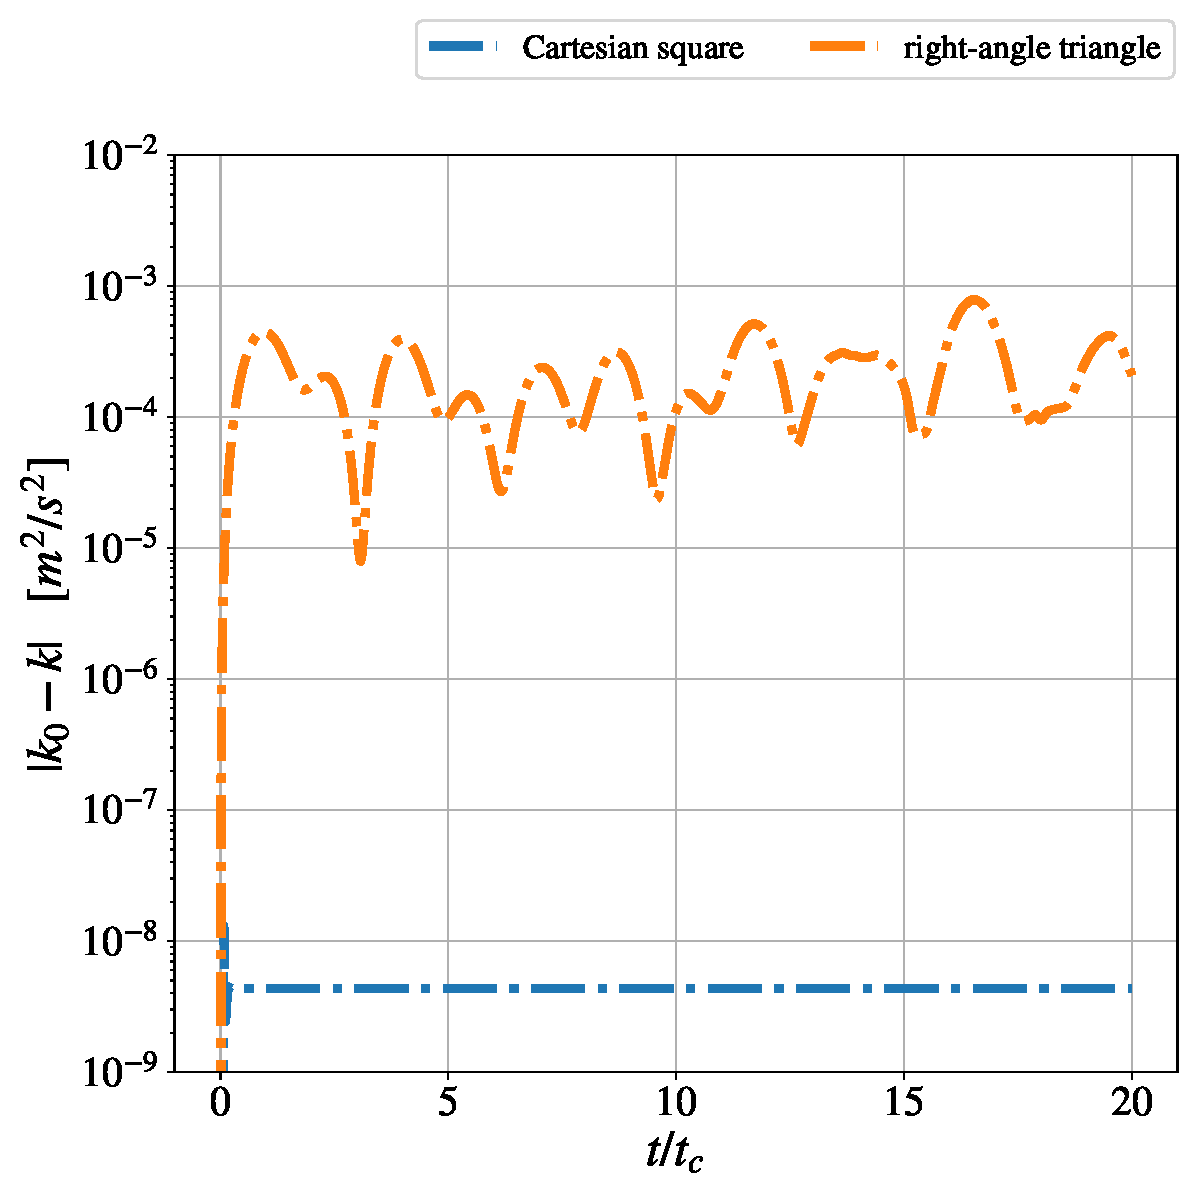
\includegraphics[width=\imgHalfWidth\columnwidth]{TGV2D/inviscid/spaeceFoamCNTGV_regular_inviscid_quadVsRAT_KEevolution_8x8_k_Log.pdf}\label{fig:TGV2D-inv-k}}
\subfloat[advection \& pressure grad. KE transport]{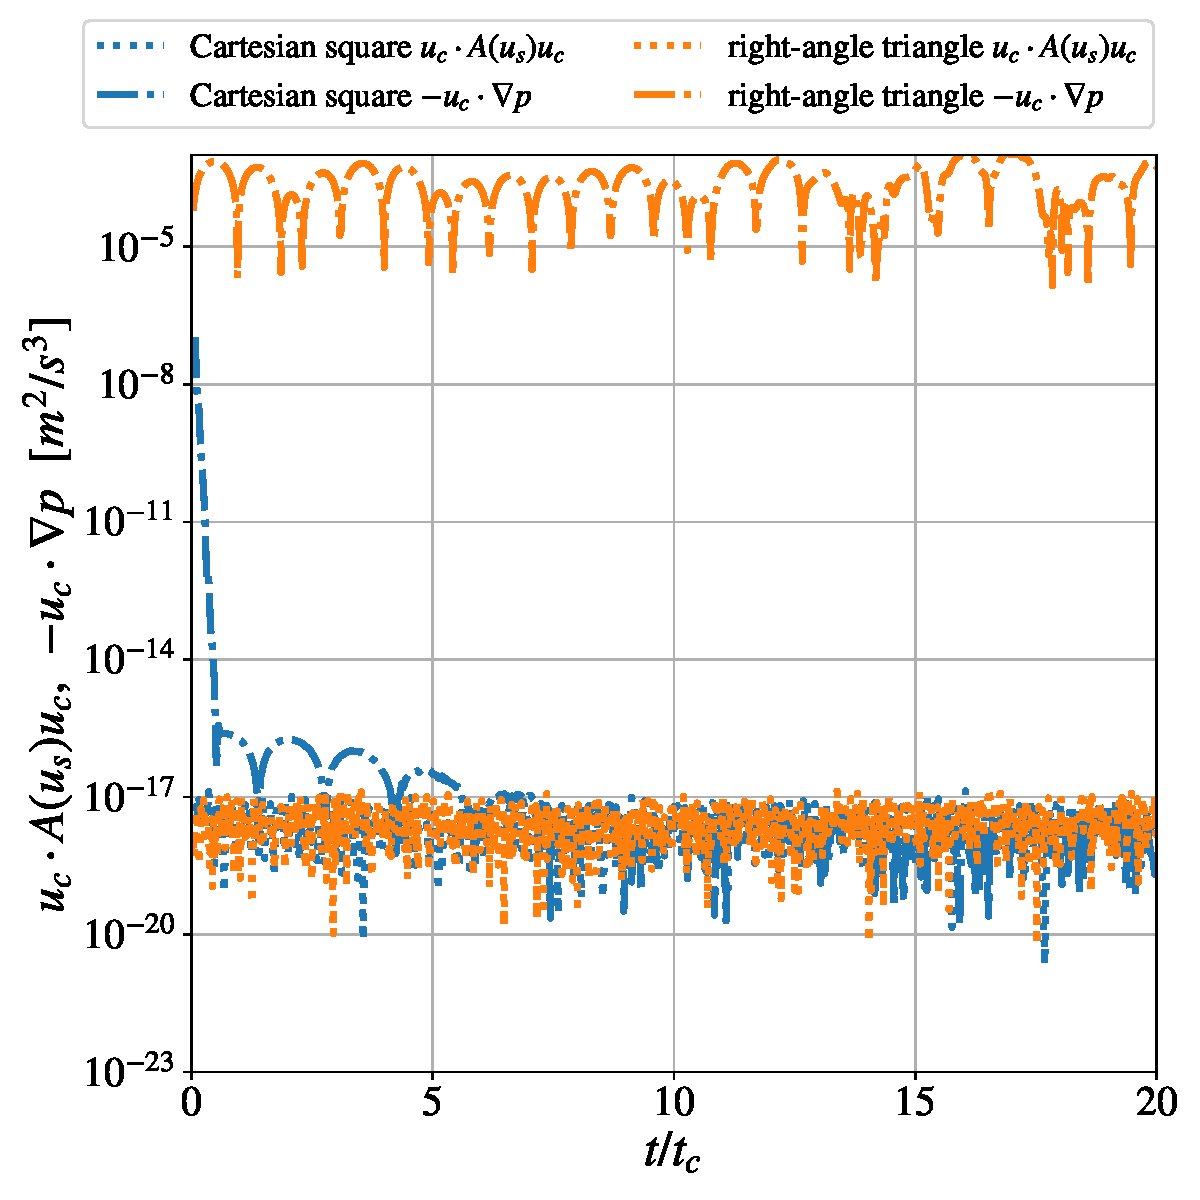
\includegraphics[width=\imgHalfWidth\columnwidth]{TGV2D/inviscid/spaeceFoamCNTGV_regular_inviscid_quadVsRAT_KEcomparison_semiLogY_advection_gradP.pdf}\label{fig:TGV2D-inv-adv}} 
\caption{Inviscid 2D Taylor-Green vortex KE, and advection and pressure gradient KE transport terms evolution comparison between a Cartesian square $65 \times 65$ mesh and a right angle triangle $(65 \times 65)\times 2$ mesh.} 
\label{fig:TGV2D-inv}
\end{figure}

For an inviscid flow $(\nu = 0)$, KE change is compared between a Cartesian square $65 \times 65$ mesh and a right-angle triangulated $(65 \times 65)\times 2$ mesh over 20 characteristic time period (Fig. \ref{fig:TGV2D-inv-k}). KE transport (Eq. \ref{eqn:KE1}) contribution from the advection term $\transDot{\avb{u}_c} \mathbf{A}(\avb{u}_f) {\avb{u}_c} $ and pressure gradient term $\transDot{\avb{u}_c} \mathbf{V}\mathbf{G}_c \avb{p}$ is also compared (Fig. \ref{fig:TGV2D-inv-adv}).

The total KE is fairly constant for both mesh types(Fig. \ref{fig:TGV2D-inv-k}). However, the right-angle triangulated mesh has higher error from initial KE $k_0$ due to a larger difference in collocated and staggered gradient operators arising from unequal control volumes and non-orthogonal correction (see pressure gradient transport term in Fig. \ref{fig:TGV2D-inv-adv}). Contribution from the advection transport term is machine zero for both mesh types.


\subsubsection{3D Taylor-Green vortex}
A 3D Taylor-Green vortex field is initialized in a cubic domain $x, y,z \in [-\pi, \pi]$ with unit characteristic length $L$ and density $\rho_0$, and characteristic velocity $U=0.1$ following the analytical expression
\begin{equation}
\begin{split}
u_0 &=U \sin \left(\frac{x}{L}\right) \cos \left(\frac{y}{L}\right) \sin \left(\frac{z}{L}\right),
\\
v_0 &=-U \cos \left(\frac{x}{L}\right) \sin \left(\frac{y}{L}\right) \sin \left(\frac{z}{L}\right), 
\\
w_0 &=0, 
\\
p_0 &=\frac{\rho_{0} U^{2}}{16} \left[\cos \left(\frac{2 x}{L}\right)+\cos \left(\frac{2 y}{L}\right)\right] \left[\cos \left(\frac{2 z}{L}\right)+2\right].
\end{split}
\end{equation}

In absence of viscosity ($\nu=0$), KE changes is compared among a Cartesian cubic $65 \times 65 \times 65$ mesh, a right-angle triangulated prism $(65 \times 65)\times 2 \times 65$ mesh and a Cartesian non-uniform hexagonal $65 \times 65 \times 65$ mesh, where control volumes are uniform at the center and nodes are clustered in the corner leading to maximum aspect ratio of 5.3. KE is fairly constant over time across all mesh types (Fig. \ref{fig:TGV3D-inv-k}) and the non-uniform hexagonal mesh has the highest error can be attributed to large pressure gradient KE transport error evident in Fig. \ref{fig:TGV3D-inv-adv}. Similar to the 2D case, contribution from the advection KE transport term is machine zero for all cases.

\begin{figure}[!h]
\centering
\subfloat[KE evolution]{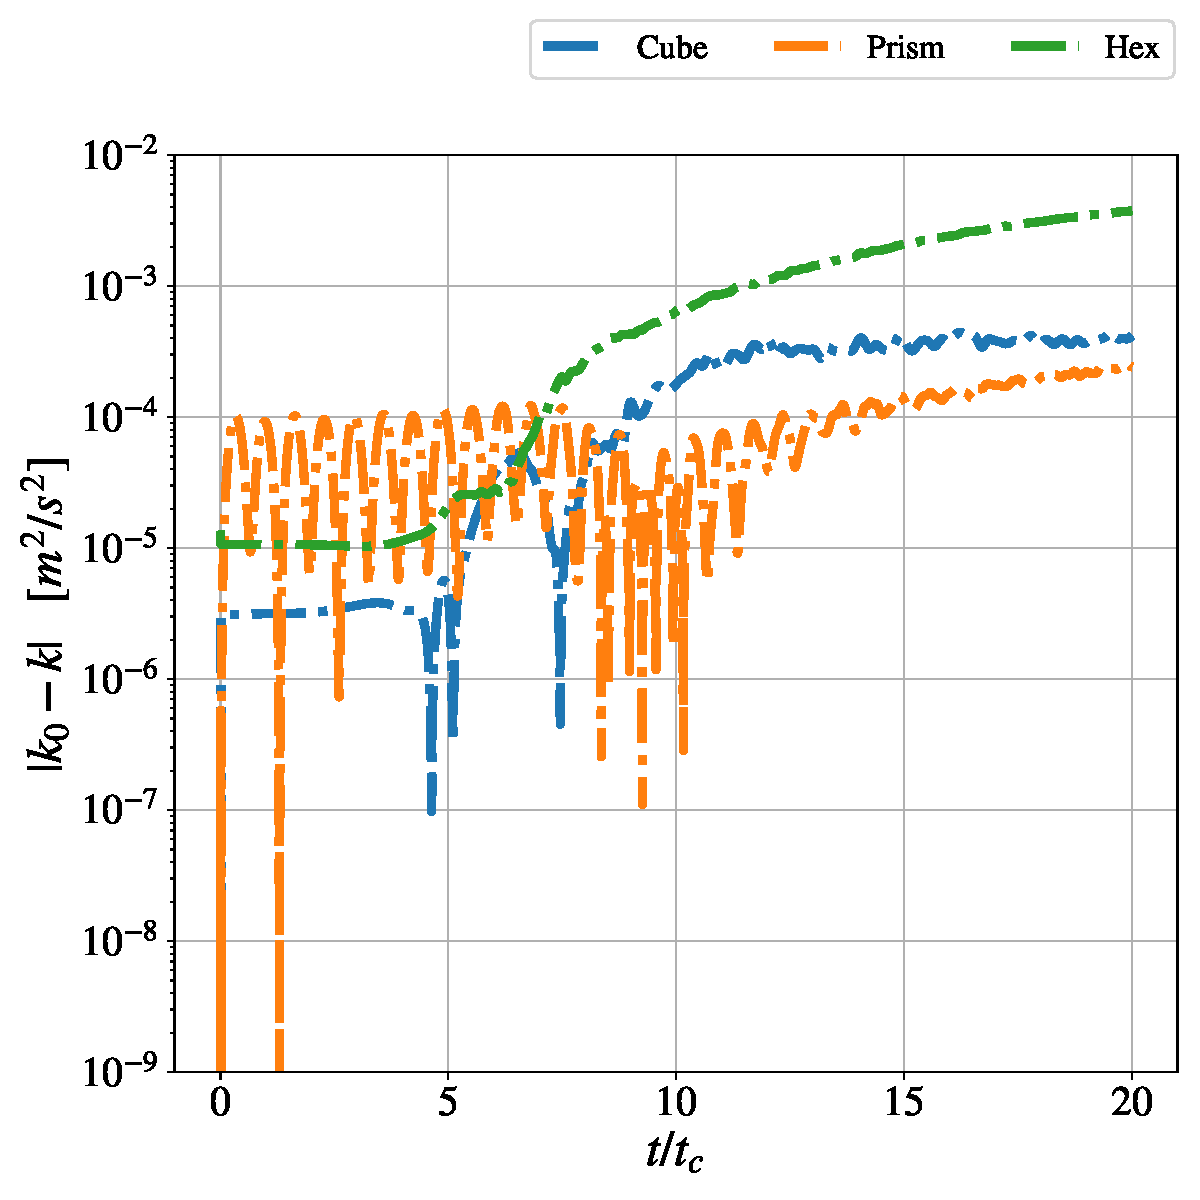
\includegraphics[width=\imgHalfWidth\columnwidth]{TGV3D/inviscid/3Mesh/spaeceFoamCNTGV_inviscid_cubeVsPrismVsHex_KEevolution_8x8_k_Log.pdf}\label{fig:TGV3D-inv-k}}
\subfloat[advection \& pressure grad. KE transport]{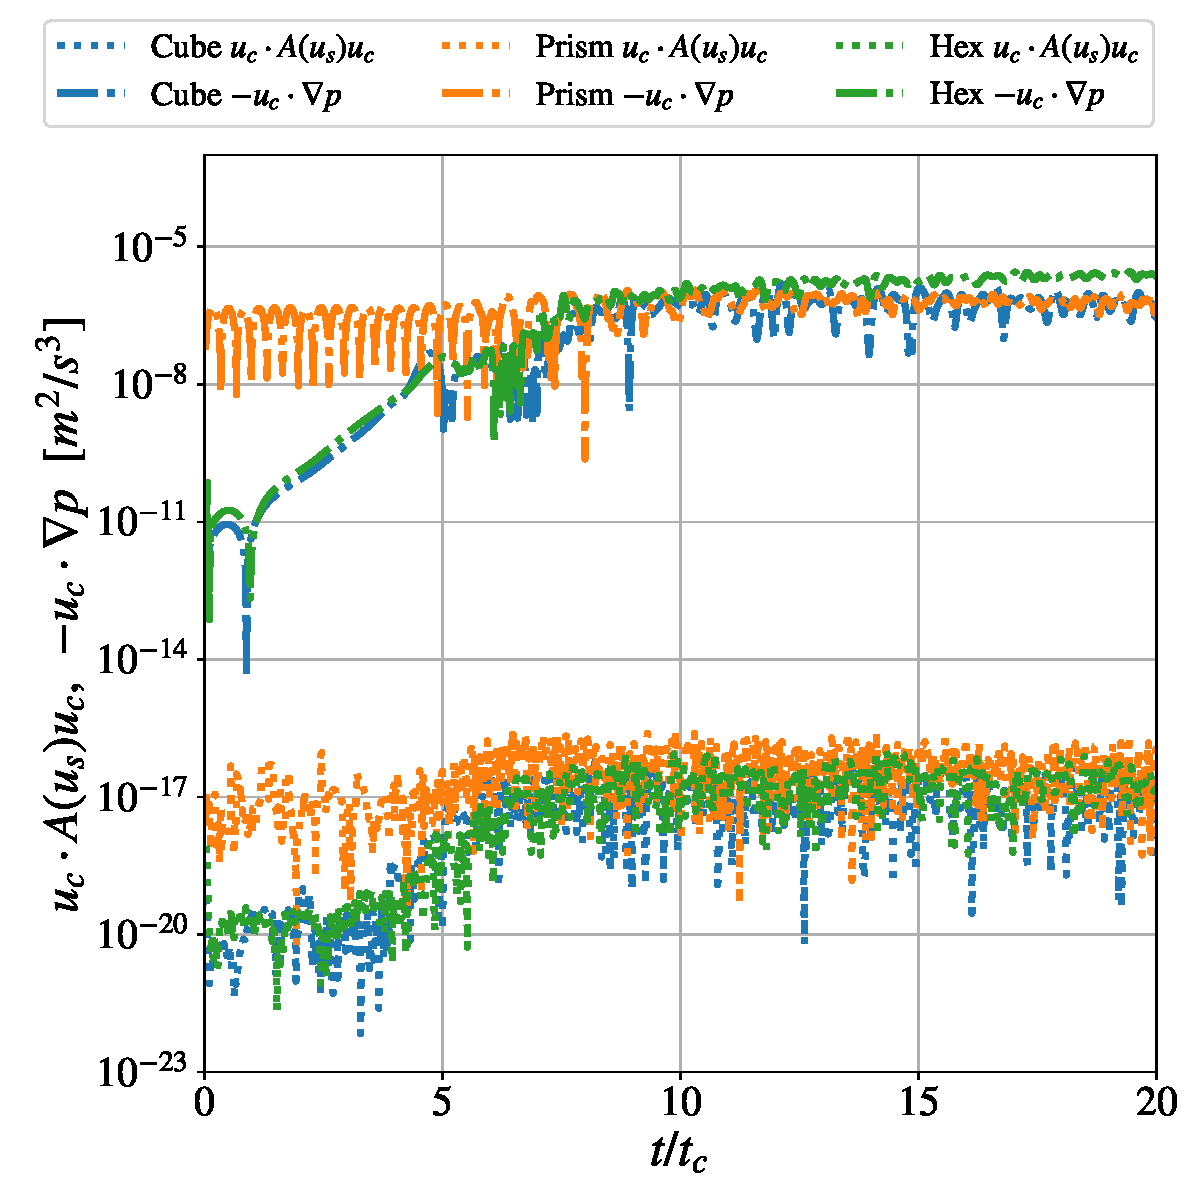
\includegraphics[width=\imgHalfWidth\columnwidth]{TGV3D/inviscid/3Mesh/spaeceFoamCNTGV_inviscid_cubeVsPrismVsHex_KEcomparison_8x8_semiLogY_advection_gradP.pdf}\label{fig:TGV3D-inv-adv}} 
\caption{Inviscid 3D Taylor-Green vortex KE, and advection and pressure gradient KE transport terms evolution comparison among three mesh types.} 
\label{fig:TGV3D-inv}
\end{figure}


To preserve (skew-)symmetry property of the discrete advection, pressure gradient and dissipation operators (Eqs. \eqref{eqn:operatorProperties}, \eqref{eqn:advOpConstraint}, \eqref{eqn:gradOpConstraint} and \eqref{eqn:LaplaceOp} respectively), the importance of using mid-point interpolation scheme is outlined. For the non-uniform Cartesian hexagonal mesh, KE evolution comparison between mid-point and linear interpolation schemes for an inviscid 3D Taylor-Green vortex is illustrated in Fig. \ref{fig:TGV3D-inv-hex}. Use of linear interpolation scheme leads to unbounded growth of the advection KE transport term and ultimately, made the linear system unstable. In contrast, the mid-point interpolation scheme kept it to machine zero and ensured solver stability.

\begin{figure}[!h]
\centering
\subfloat[KE evolution]{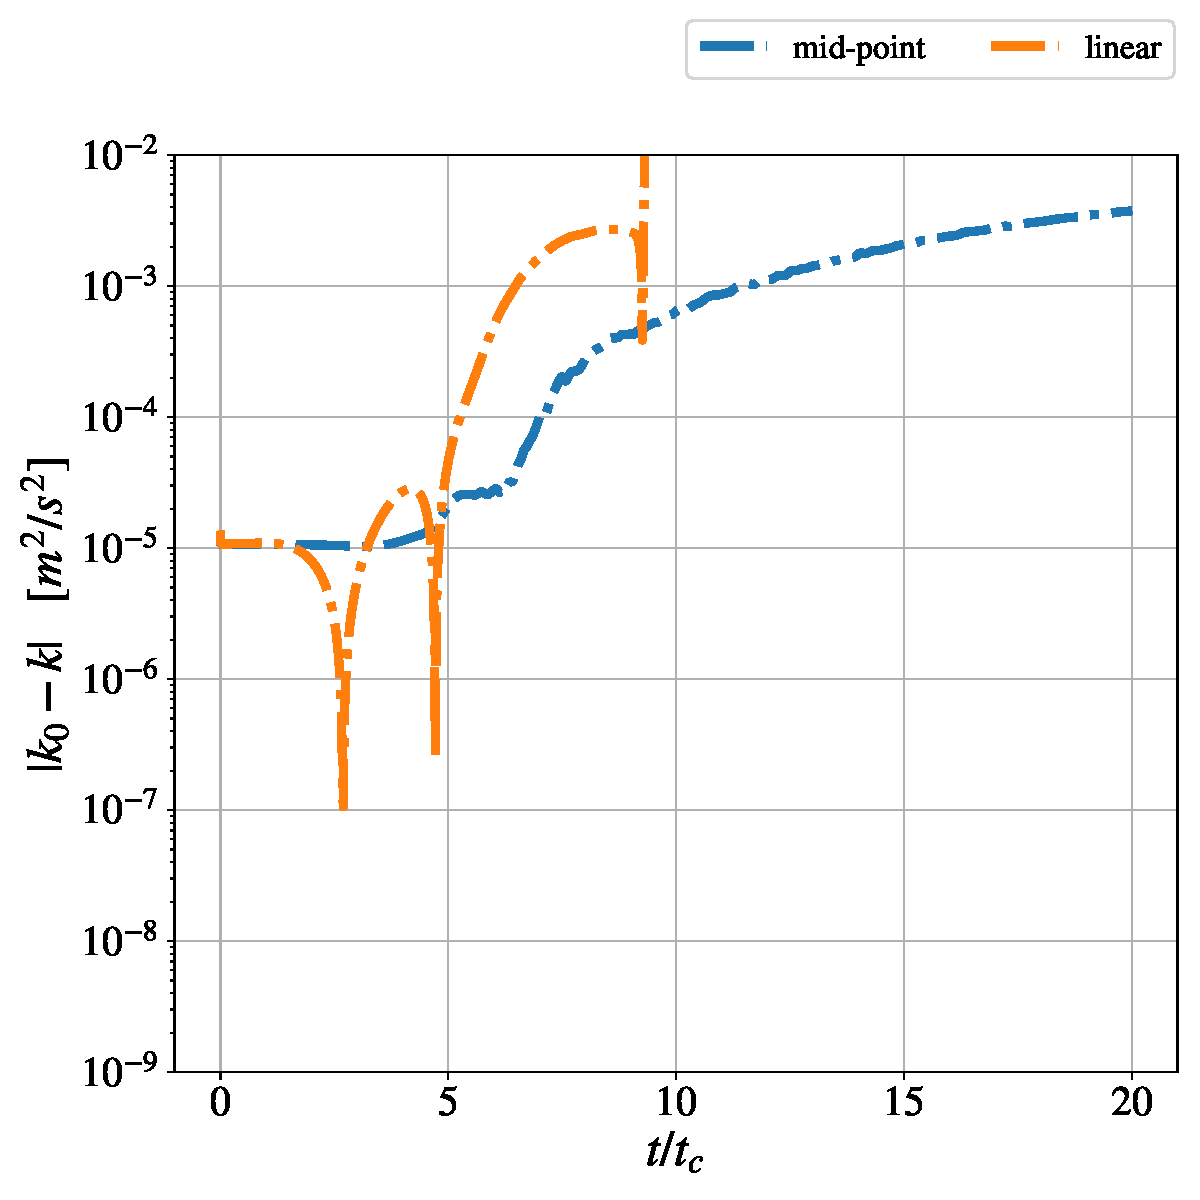
\includegraphics[width=\imgHalfWidth\columnwidth]{TGV3D/inviscid/midpointVsLinear/spaeceFoamCNTGV_inviscid_midpointVsLinear_KEevolution_8x8_k_Log.pdf}\label{fig:TGV3D-inv-hex-k}}
\subfloat[advection \& pressure grad. KE transport]{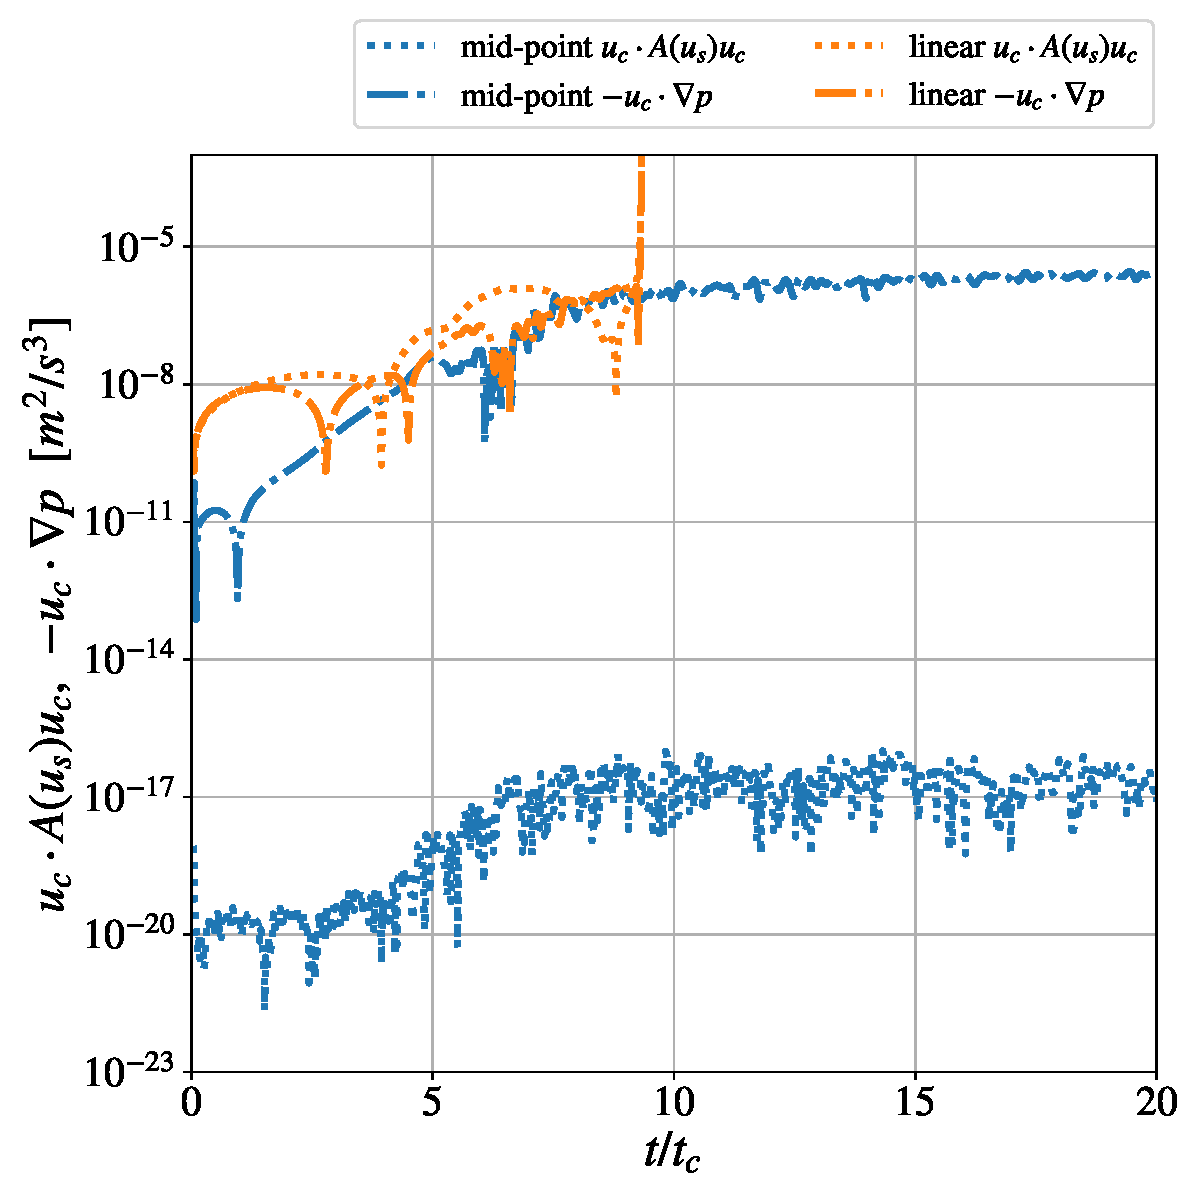
\includegraphics[width=\imgHalfWidth\columnwidth]{TGV3D/inviscid/midpointVsLinear/spaeceFoamCNTGV_inviscid_midpointVsLinear_KEcomparison_8x8_semiLogY_advection_gradP.pdf}\label{fig:TGV3D-inv-hex-adv}} 
\caption{Inviscid 3D Taylor-Green vortex KE, and advection and pressure gradient KE transport terms evolution comparison between midpoint and linear interpolation schemes for the Cartesian non-uniform hexagonal $65 \times 65 \times 65$ mesh.} 
\label{fig:TGV3D-inv-hex}
\end{figure}



\clearpage
\subsubsection{Influence of A6 regularization}
\label{sec:A6KEconserv}

In Sec. \ref{sec:advReg}, we have identified that the in-exact shift-operators lead to higher divergence error for the residual-filtered face-velocity $\avbPrime{u_f}$, which ultimately break KE conservation. In Fig. \ref{fig:TGV3D-inv-A6}, KE evolution and KE transport contribution from the advection and pressure gradient terms are compared among the \spaece, \spaeceA and \spaeceAdivFree algorithms in a Cartesian non-uniform hexagonal $65 \times 65 \times 65$ mesh. The \spaeceAdivFree and \spaece algorithms conserve KE energy and the advection term is close to machine zero. The KE for the \spaeceA algorithm gradually diverges (Fig. \ref{fig:TGV3D-inv-A6-k}) dueto accumulation of large, non-zero advection transport term (Fig. \ref{fig:TGV3D-inv-A6-adv}). Overall, in a collocated mesh formulation the \spaeceAdivFree maintains KE conservation, while \spaeceA introduce non-zero advection KE transport term.

\begin{figure}[!h]
\centering
\subfloat[KE evolution]{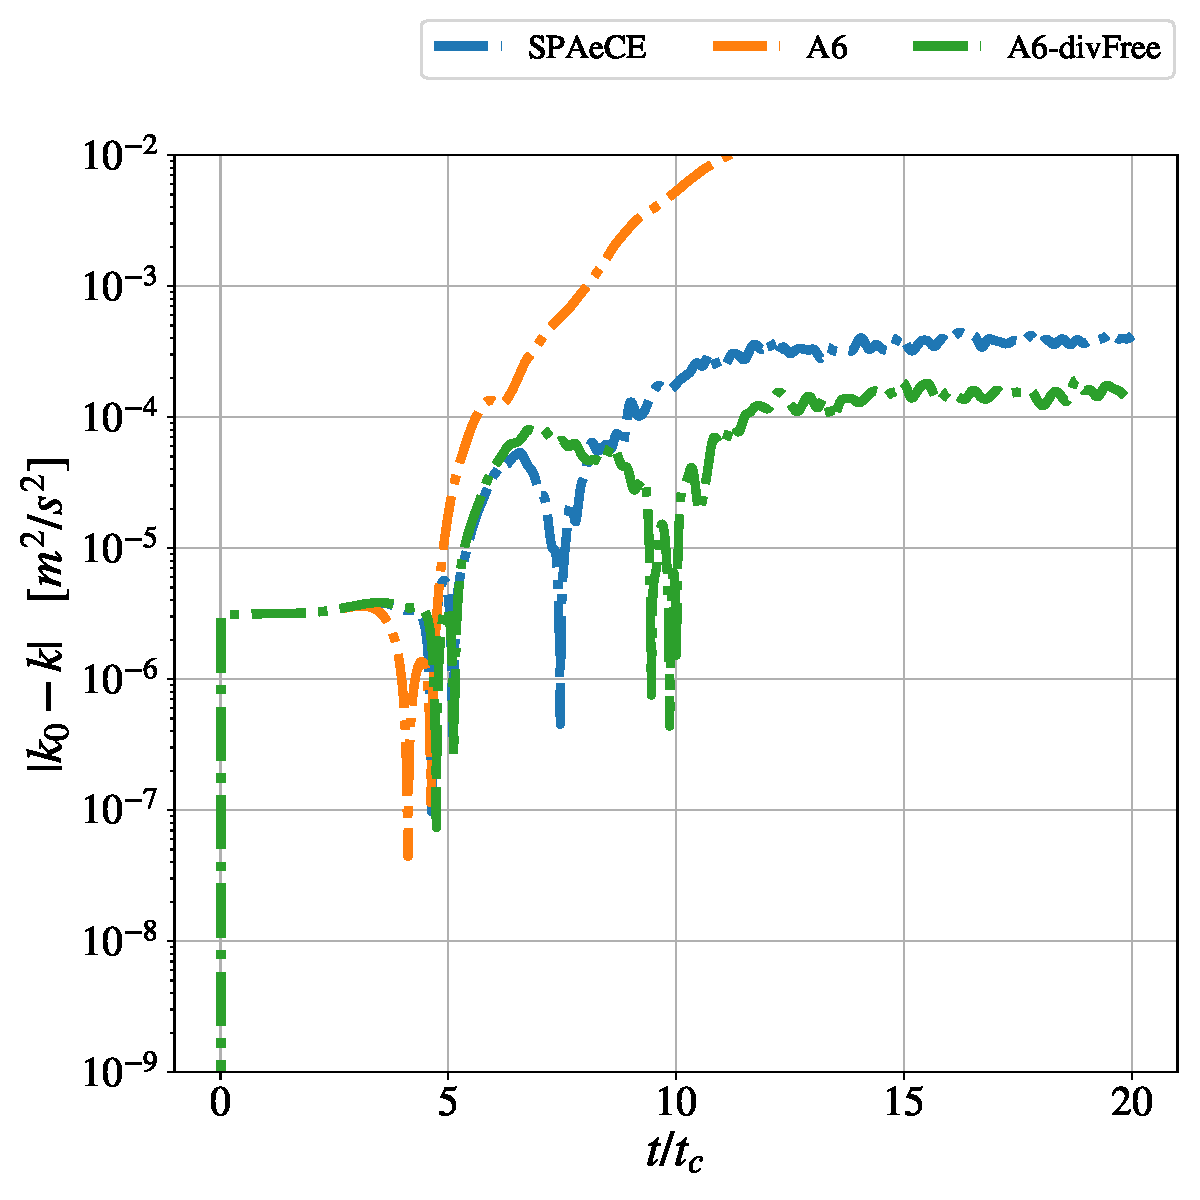
\includegraphics[width=\imgHalfWidth\columnwidth]{TGV3D/inviscid/A6phiResCorrVsA6phiDivFree/spaeceFoamCNTGV_inviscid_A6phiCorrvsA6divFree_KEevolution_8x8_k_Log.pdf}\label{fig:TGV3D-inv-A6-k}}
\subfloat[advection \& pressure grad. KE transport]{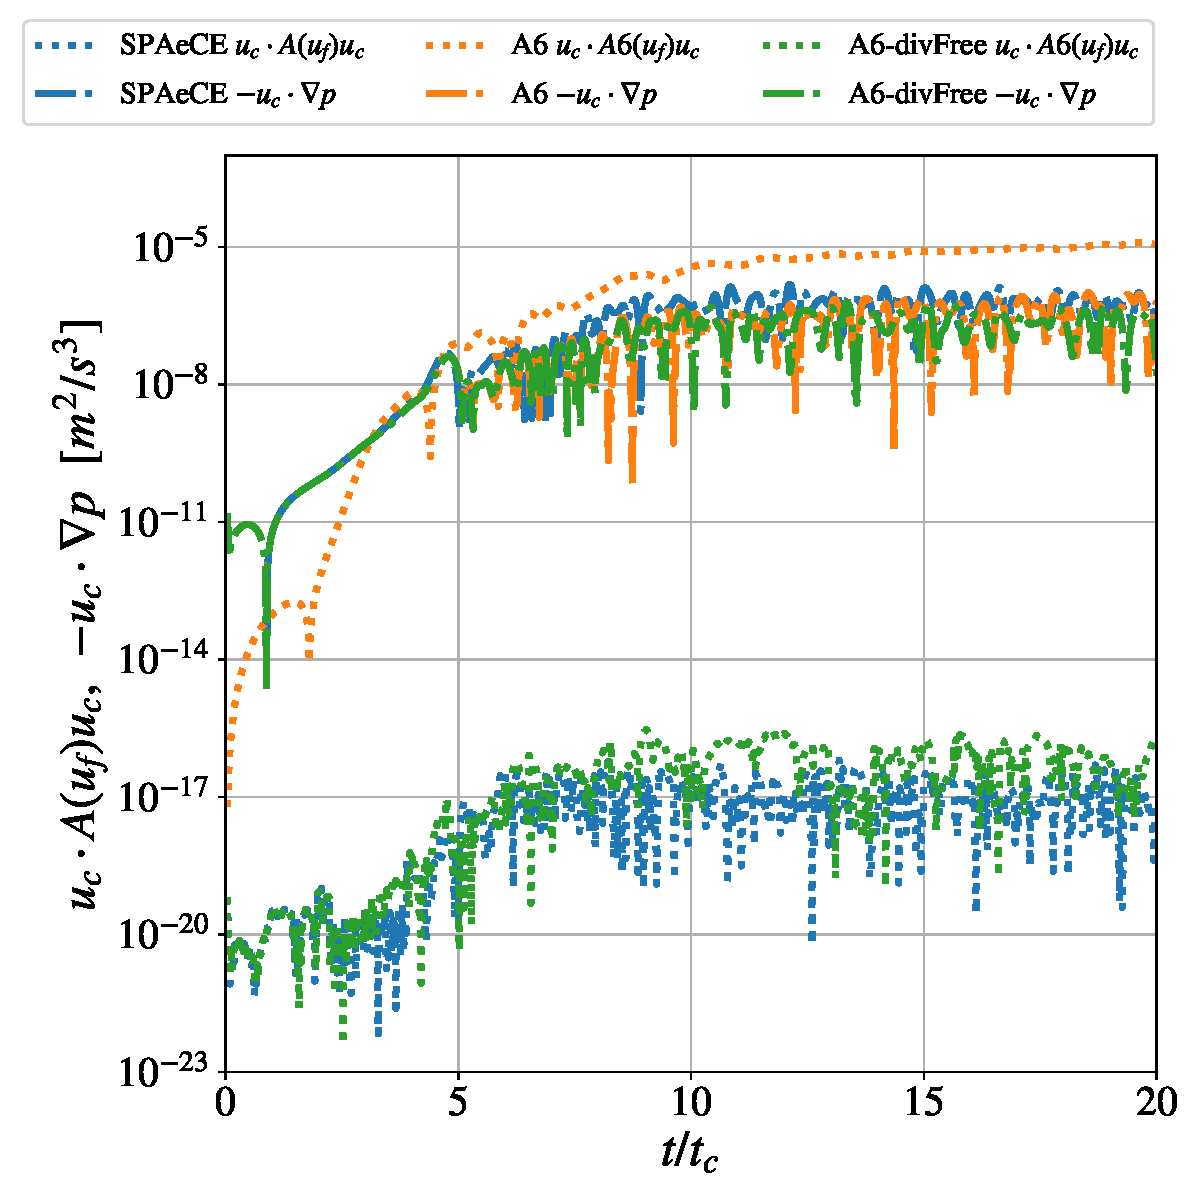
\includegraphics[width=\imgHalfWidth\columnwidth]{TGV3D/inviscid/A6phiResCorrVsA6phiDivFree/spaeceFoamCNTGV_inviscid_A6phiCorrvsA6divFreeKEcomparison_8x8_semiLogY_advection_gradP.pdf}\label{fig:TGV3D-inv-A6-adv}} 
\caption{Inviscid 3D Taylor-Green vortex KE, and advection and pressure gradient KE transport terms evolution comparison among the \spaece, \spaeceA and \spaeceAdivFree algorithms in a Cartesian non-uniform hexagonal $65 \times 65 \times 65$ mesh} 
\label{fig:TGV3D-inv-A6}
\end{figure}







\clearpage
\newpage
\subsection{Order of convergence}
\label{sec:orderOfCon}
\subsubsection{Order of convergence without Rhie-Chow correction}
A viscous 2D Taylor-Green vortex case, applying same domain and initialization as the invicisd case described in section \ref{sec:TGV2d-inv}, but with $Re=1\times10^3,\quad \nu = 1\times10^{-3}$ which dictates the flow as \textit{laminar}. The discrete differential operators are discretized with a Crank-Nicolson temporal scheme and 2nd order central difference spatial schemes with mid-point interpolation. The linear systems are solved for a tolerance of $1\times10^{-15}$. Flow is simulated for $t/t_c = 1.12$ time for all cases and error norms are reported in Fig. \ref{fig:TGV2D-Cart1000-spaece}. 

\begin{figure}[!h]
\centering
\subfloat[Temporal convergence ($257 \times 257$ mesh)]{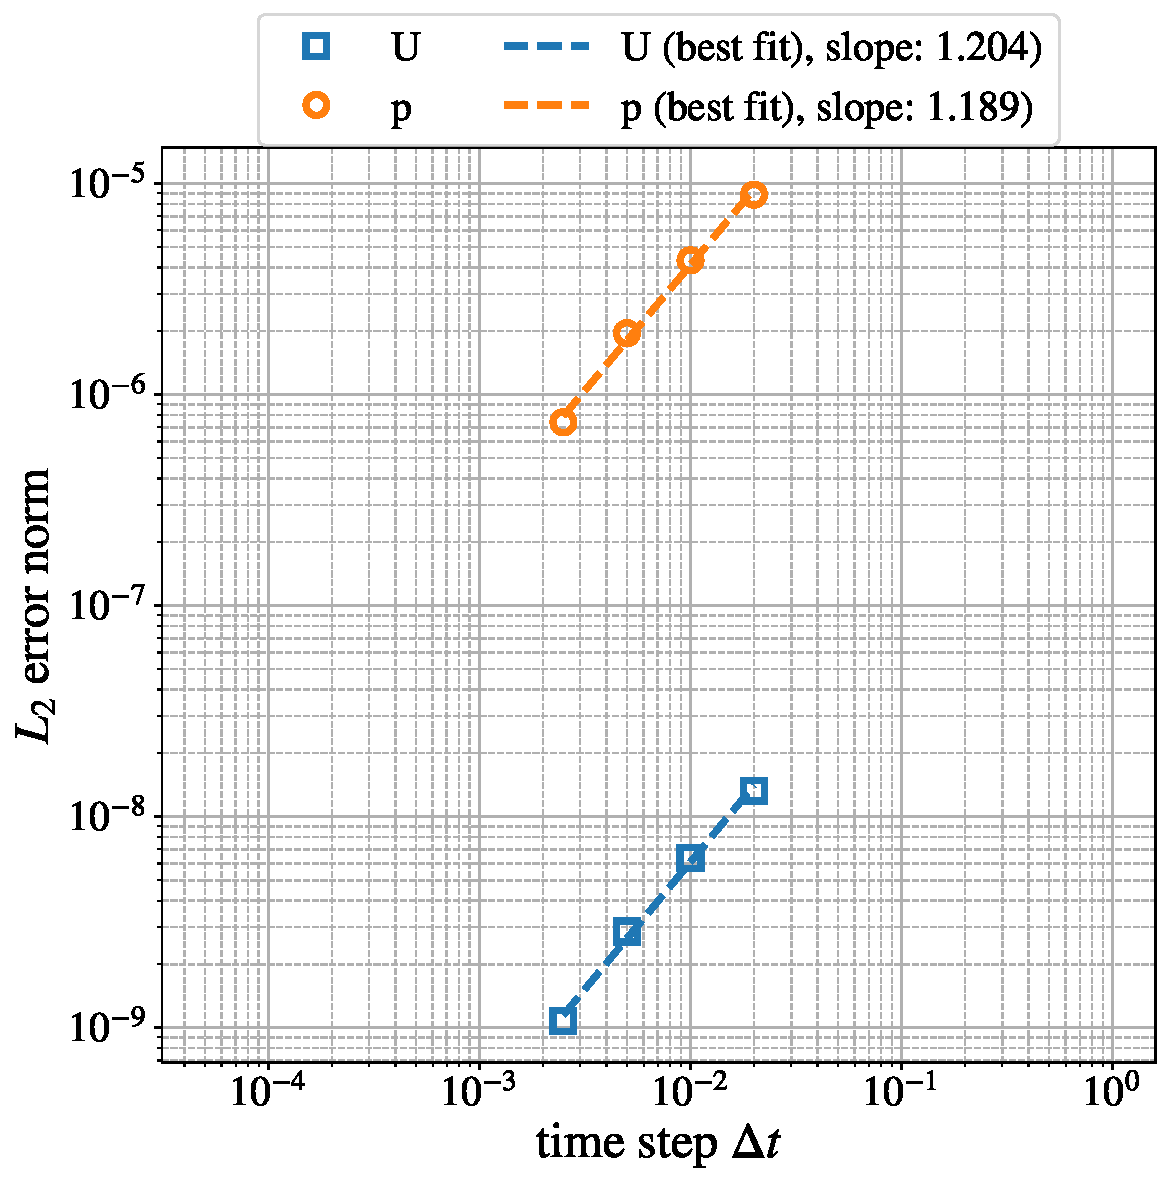
\includegraphics[width=\imgHalfWidth\columnwidth]{TGV2D/Re1000/Cartesian/spaeceFoamCNTGV/regular/temporalConvergence/spaeceFoamCNTGV_Re1000_regular_257x257_log_2ndErrorNorm_refTime_1_12.pdf}\label{fig:TGV2D-Cart1000-spaece-tempCon}}
\subfloat[Spatial convergence (time step $0.001s$)]{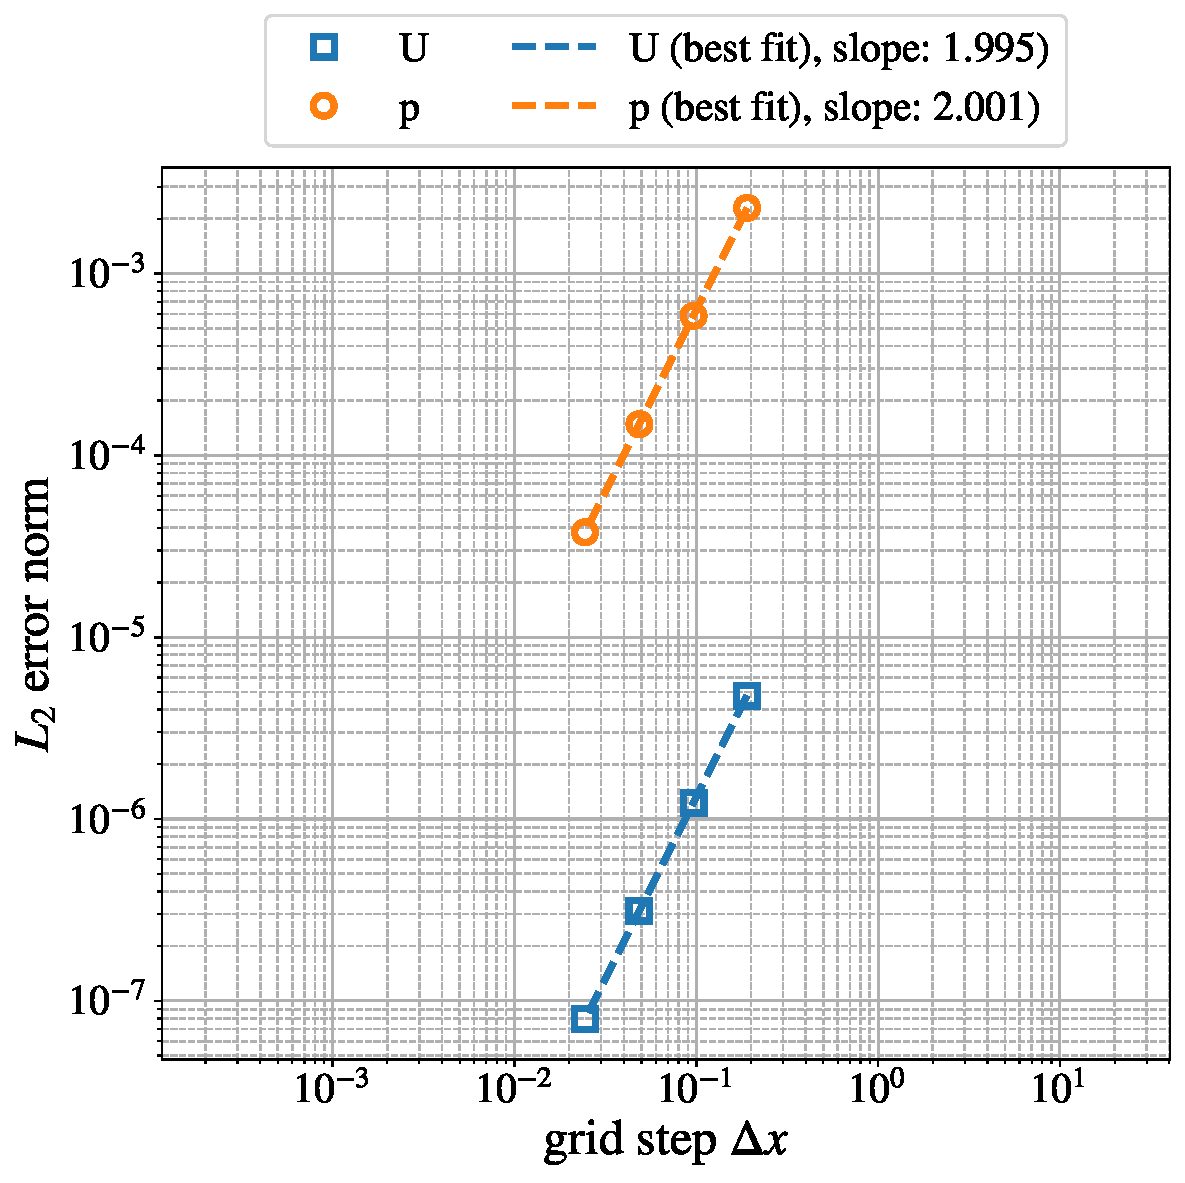
\includegraphics[width=\imgHalfWidth\columnwidth]{TGV2D/Re1000/Cartesian/spaeceFoamCNTGV/regular/gridConvergence/spaeceFoamCNTGV_Re1000_regular_1e-3_2ndErrorNorm.pdf}\label{fig:TGV2D-Cart1000-spaece-spatCon}} 
\caption{Temporal and spatial error norms convergence of the \spaece algorithm for a 2D Taylor-Green vortex with $Re=1\times10^3$ simulated in Cartesian square meshes} 
\label{fig:TGV2D-Cart1000-spaece}
\end{figure}

To determine the temporal convergence rate, flow is simulated on a Cartesian square $257 \times 257$ mesh for a series of time steps $0.02, 0.01, 0.005 $ and $0.0025$. To isolate the spatial discretization error, a reference simulation is performed with time step $1\times10^{-3}$ and reference error norms are subtracted from error norms of larger time steps. The temporal convergence for $L_2$ error norms is 1st order accurate (Fig. \ref{fig:TGV2D-Cart1000-spaece-tempCon}). Although, the Crank-Nicolson scheme is 2nd order accurate, the inherent splitting error of the \spaece algorithm is first order accurate and when combined with 2nd order temporal schemes delivered 1st order temporal convergence only. The pressure error norms are about $1\times10^3$ times higher than the velocity error norms.

Spatial error convergence rate is determined by simulating the flow in four Cartesian square meshes: $33 \times 33$, $65 \times 65$, $127 \times 127$ and $257 \times 257$. To keep the temporal discretization error minimal, a small time-step $1\times10^{-3}s$ is used for all cases. The spatial convergence rate for $L_2$ error norms is 2nd order accurate (Fig. \ref{fig:TGV2D-Cart1000-spaece-spatCon}) and the pressure error norms are approximately $300$ times higher than the velocity error norms. The $L_\infty$ error norms are not reported, but has the same temporal and spatial convergence order as the $L_2$ error norms. 


\subsubsection{Order of convergence with Rhie-Chow correction}
\label{sec:OoC-RC}
To avoid checkerboard like pattern, simulations are performed with Rhie-Chow correction\cite{rhie1983} for face-normal velocity (Eq. \eqref{eqn:updateUfRC}). Fig. \ref{fig:TGV2D-Cart1000-spaeceRC} illustrates the temporal and spatial error convergence for the \spaece algorithm with Rhie-Chow correction (\spaeceRC) evaluated for the same 2D Taylor-Green vortex of $Re\,1\times10^3$ case.
\begin{figure}[!h]
\centering
\subfloat[Temporal convergence]{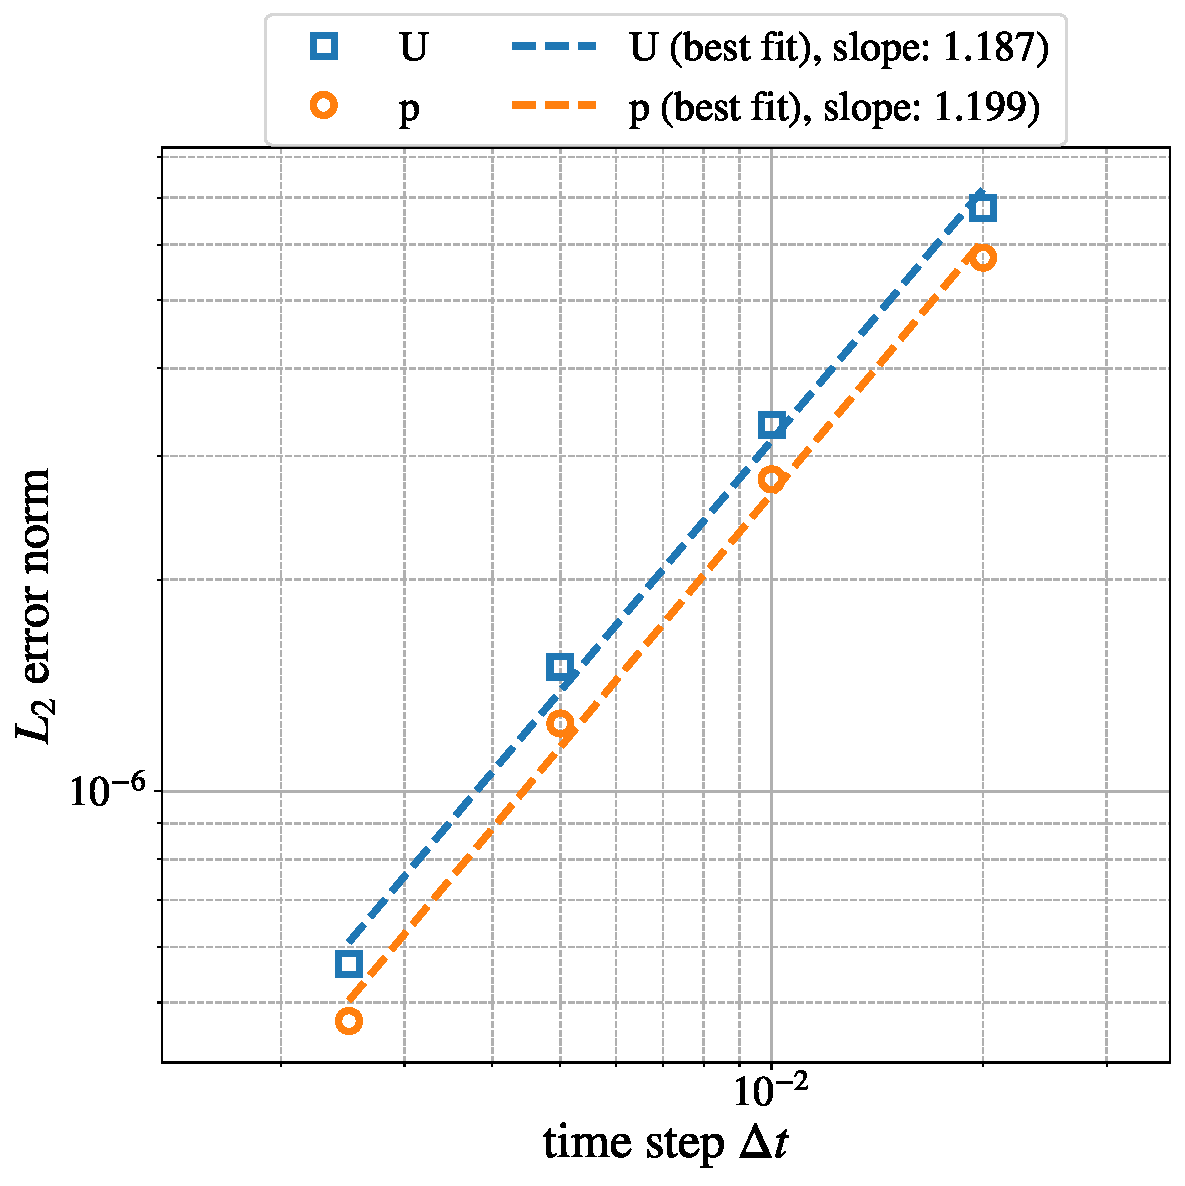
\includegraphics[width=\imgHalfWidth\columnwidth]{TGV2D/Re1000/Cartesian/spaeceFoamCNTGV/regularRC/temporalConvergence/spaeceFoamCNTGV_Re1000_regularRC_257x257_log_2ndErrorNorm_refTime_1_12.pdf}\label{fig:TGV2D-Cart1000-spaeceRC-tempCon}}
\subfloat[Spatial convergence]{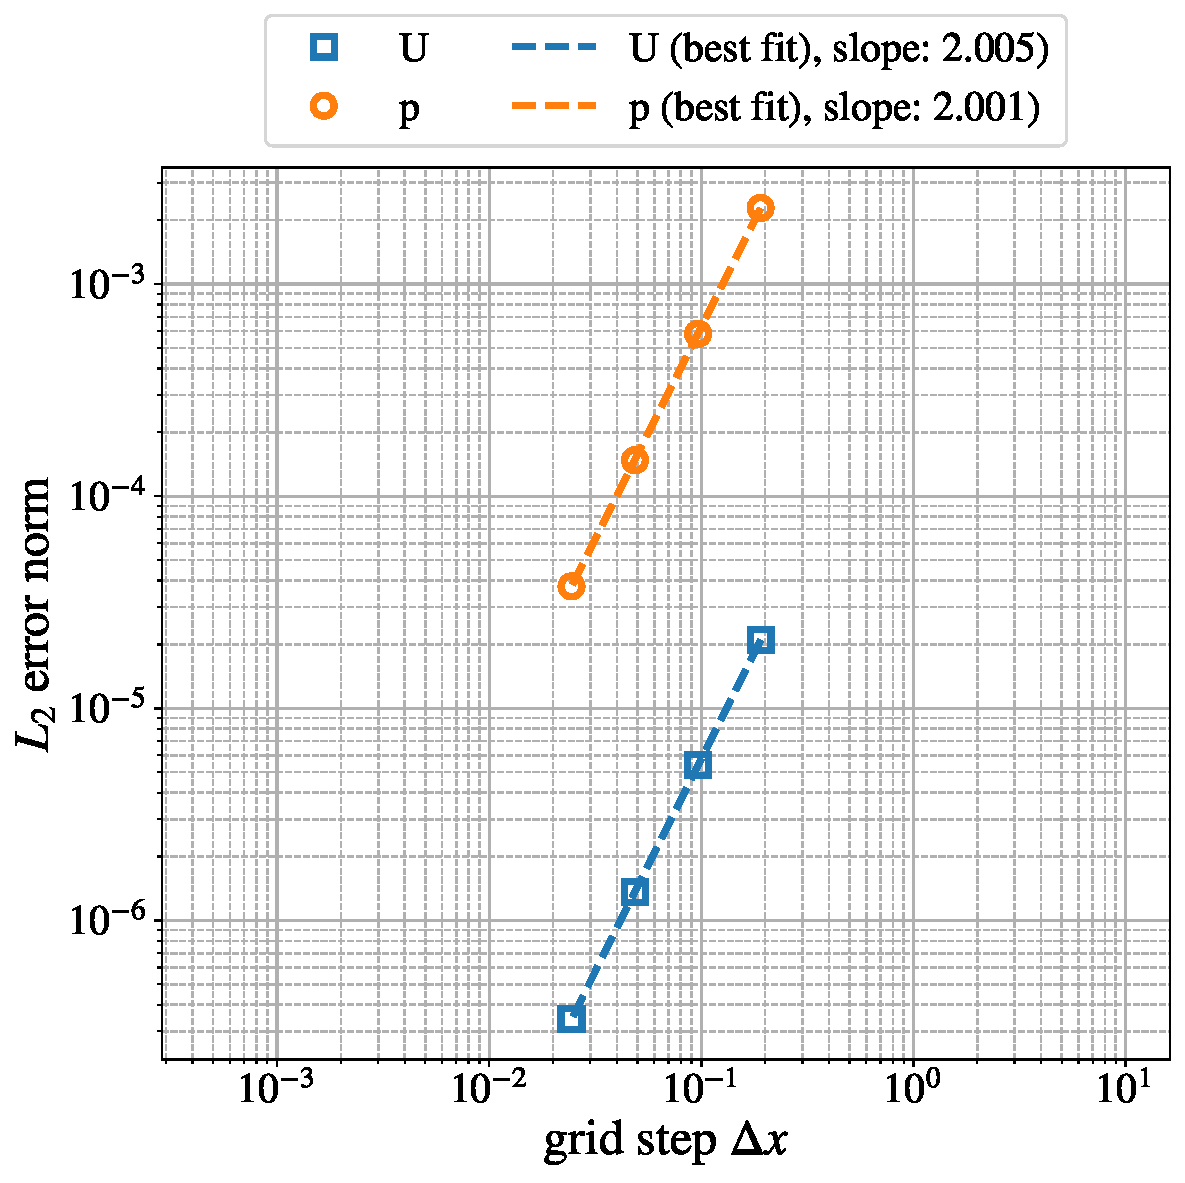
\includegraphics[width=\imgHalfWidth\columnwidth]{TGV2D/Re1000/Cartesian/spaeceFoamCNTGV/regularRC/gridConvergence/spaeceFoamCNTGV_Re1000_regularRC_1e-3_2ndErrorNorm.pdf}\label{fig:TGV2D-Cart1000-spaeceRC-spatCon}} 
\caption{Temporal and spatial error norms convergence of the \spaeceRC algorithm for a 2D Taylor-Green vortex with $Re\,1\times10^3$ simulated in Cartesian square meshes} 
\label{fig:TGV2D-Cart1000-spaeceRC}
\end{figure}

The temporal error convergence remained 1st order accurate, while the velocity error magnitudes are increased to pressure error levels (Fig. \ref{fig:TGV2D-Cart1000-spaeceRC-tempCon}). The spatial error convergence rate is also maintained 2nd order convergence with increased velocity error (Fig. \ref{fig:TGV2D-Cart1000-spaeceRC-spatCon}). The $L_\infty$ error norms produced same order of convergence as the $L_2$ error norms, thus not reported.
%

The \piso algorithm implementation in OpenFOAM \cite{weller1998} has an indirect implementation of the Rhie-Chow correction, where the staggered velocity is updated excluding the pressure gradient. It requires significant change in staggered velocity update (Eq. \eqref{eqn:updateUfRC}), Poisson pressure solve (Eq. \eqref{eqn:poissonPressure}) and velocity correction (Eq. \eqref{eqn:updateFaceVel}) equations: 
\begin{align}
\begin{split}
\text{Update face-normal velocity: } & 
\avb{u}_f^{n+1, *} = \shiftCS \left[\mathcal{A_F}^{-1} ( \mathcal{H} + \mathcal{S}) \right] \cdot \faceUnitNormal,
\\
\text{Poisson pressure solve: } & \mathcal{L} \mathcal{A_F}^{-1}  \, \avb{p}_c = \mathcal{M} \avb{u}_f^{n+1,*},
\\
\text{Correct face-normal velocity: } & \avb{u}_f^{n+1} = \avb{u}_f^{n+1, *} - \mathcal{A_F}^{-1} \, \mathcal{G_F}\avb{p}_c .
\end{split}
\label{eqn:openfoamPiso}
\end{align}

\begin{figure}[!h]
\centering
\subfloat[temporal convergence]{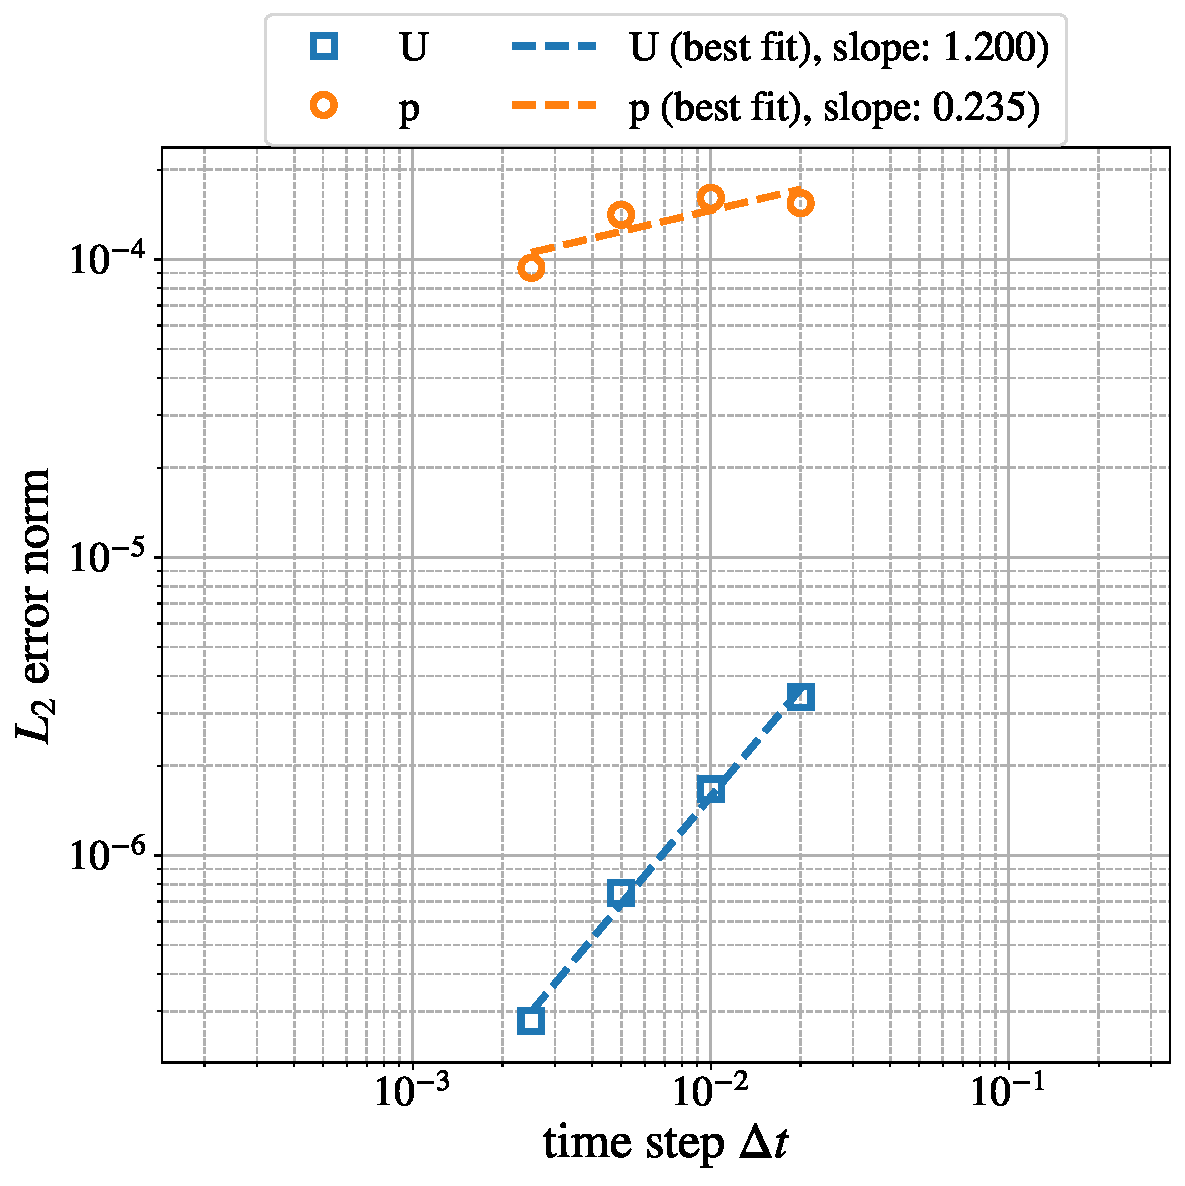
\includegraphics[width=\imgHalfWidth\columnwidth]{TGV2D/Re1000/Cartesian/pisoFoamwoDdtCorr/CN1/temporalConvergence/pisoFoamwoDdtCorr_Re1000_CN1_257x257_log_2ndErrorNorm_refTime_1_12.pdf}\label{fig:TGV2D-Cart1000-piso-tempCon}}
\subfloat[spatial convergence]{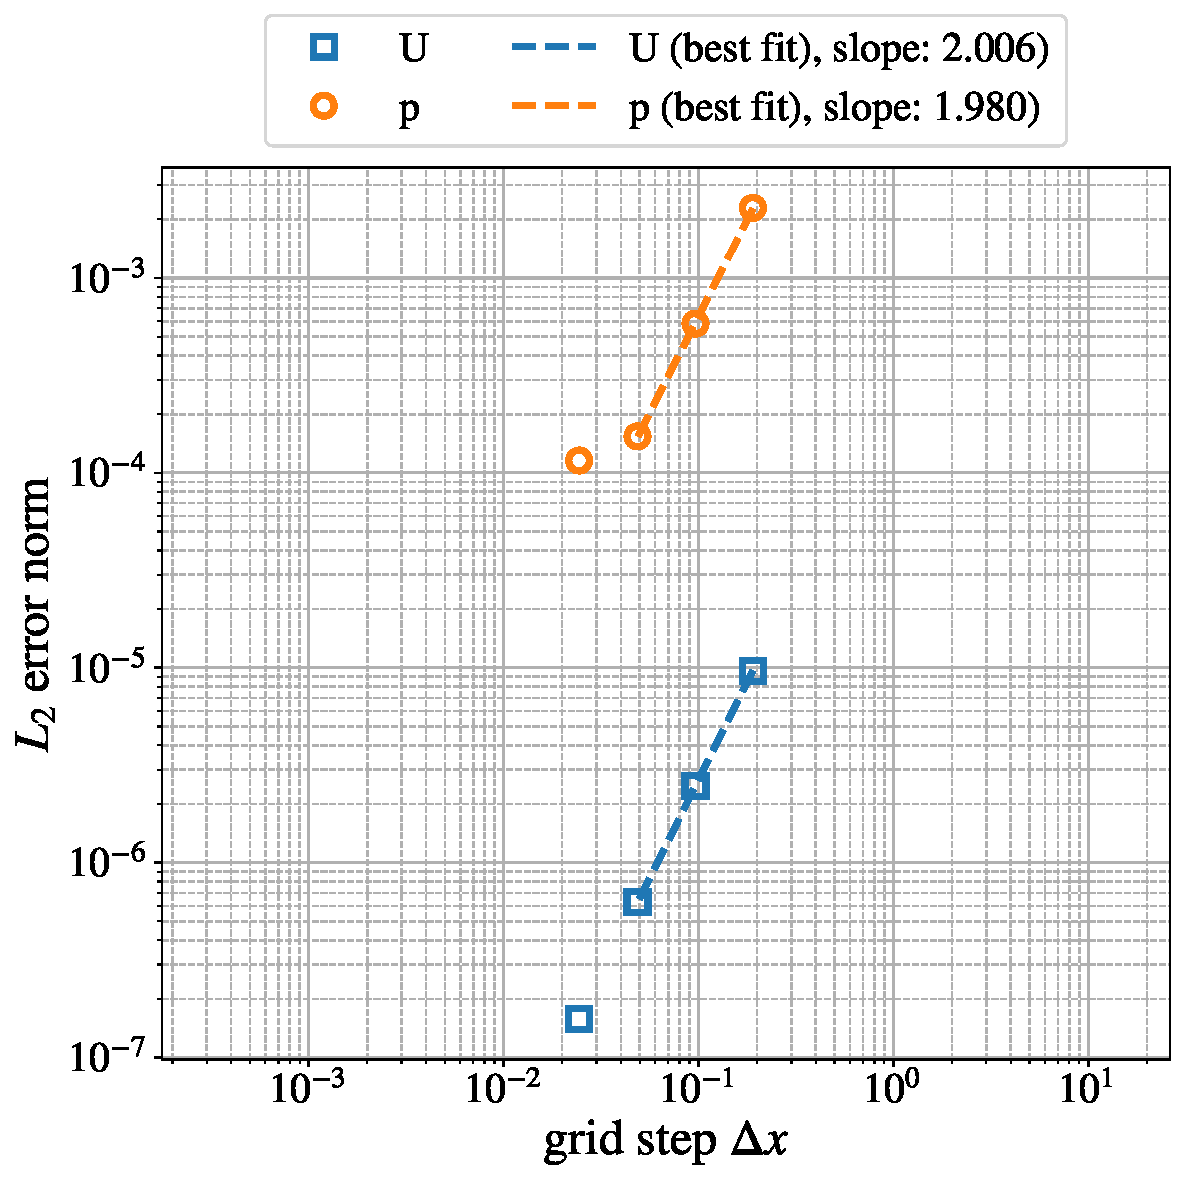
\includegraphics[width=\imgHalfWidth\columnwidth]{TGV2D/Re1000/Cartesian/pisoFoamwoDdtCorr/CN1/gridConvergence/pisoFoamwoDdtCorr_Re1000_CN1_1e-3_2ndErrorNorm.pdf}\label{fig:TGV2D-Cart1000-piso-spatCon}} 
\caption{Temporal and spatial error norms convergence of the OpenFOAM \piso algorithm (without  Rhie-Chow correction for time step) for a 2D Taylor-Green vortex with $Re\,1\times10^3$ simulated in Cartesian square meshes.} 
\label{fig:TGV2D-Cart1000-piso}
\end{figure}

Following the \spaeceRC algorithm validation, temporal and spatial error convergence for OpenFOAM \piso algorithm implementation (with two pressure solve iterations and without Rhie-Chow correction for time-step \footnote{The authors observed that the Rhie-Chow correction for time-step introduces excessive artificial dissipation, often appeared as the largest source of dissipation. To facilitate comparison with the \spaeceRC and \spaeceARC algorithms, the  Rhie-Chow correction for time-step is excluded from the OpenFOAM \piso algorithm.}) is illustrated in Fig. \ref{fig:TGV2D-Cart1000-piso}. The temporal convergence for velocity is first order, but pressure is close to zeroth order(Fig. \ref{fig:TGV2D-Cart1000-piso-tempCon}). Both the velocity and pressure fields demonstrated a 2nd order convergence for spatial error norms (Fig. \ref{fig:TGV2D-Cart1000-piso-spatCon}). The $L_\infty$ error norms of the \piso algorithm delivered same order of convergence as the $L_2$ error norms.

\begin{figure}[!ht]
\centering
\subfloat[$L_2$ error norm]{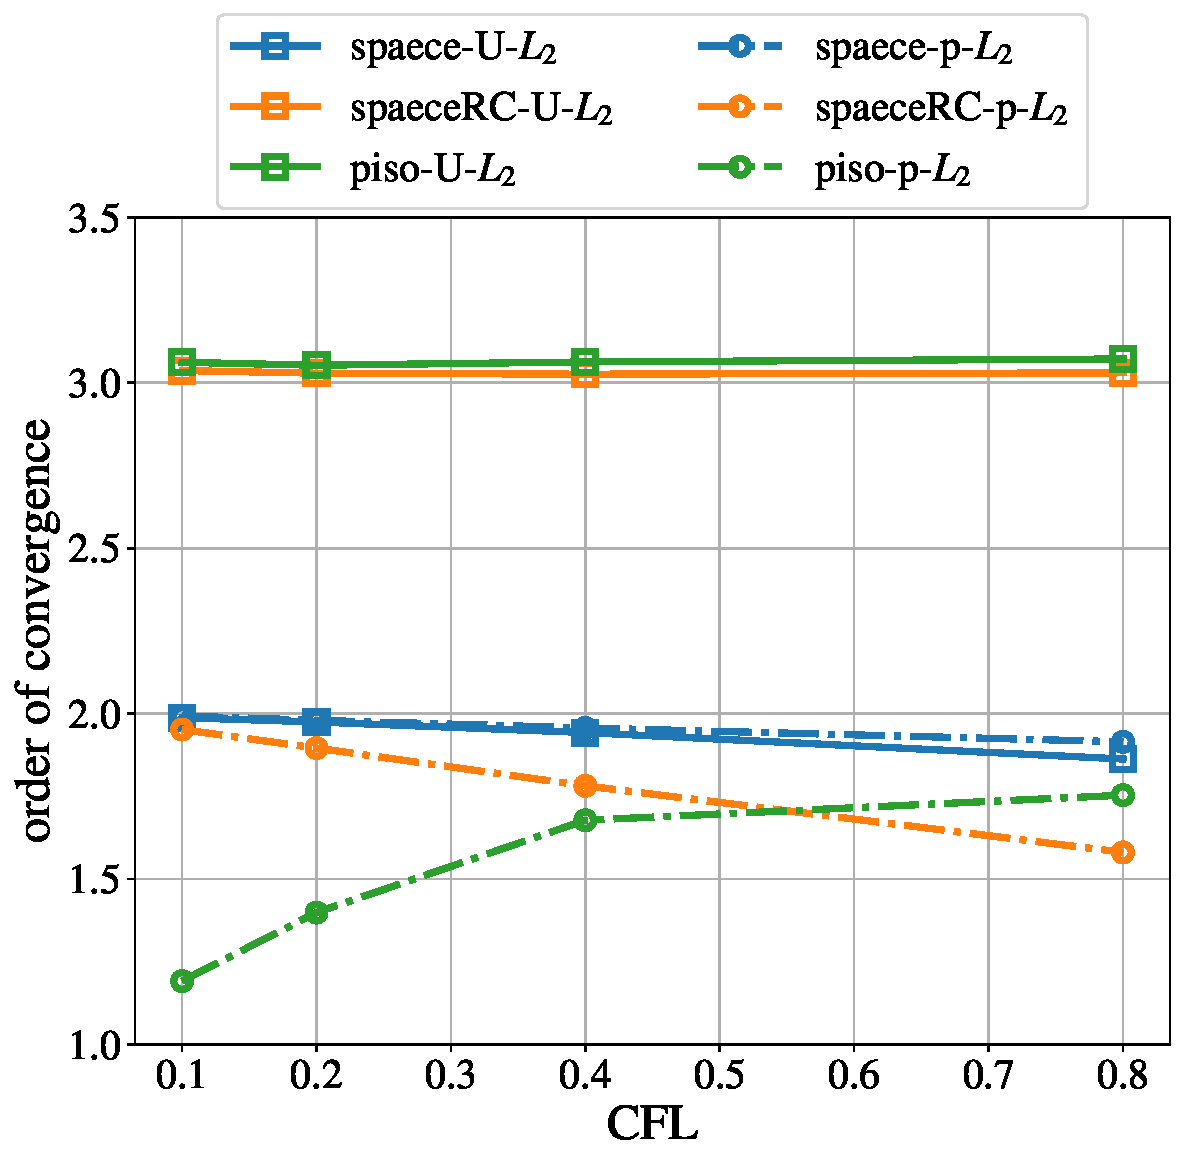
\includegraphics[width=\imgHalfWidth\columnwidth]{TGV2D/Re1000/Cartesian/ErrorNormComp_2nd.pdf}\label{fig:TGV2D-Cart1000-CFL-2nd}}
\subfloat[$L_\infty$ error norm]{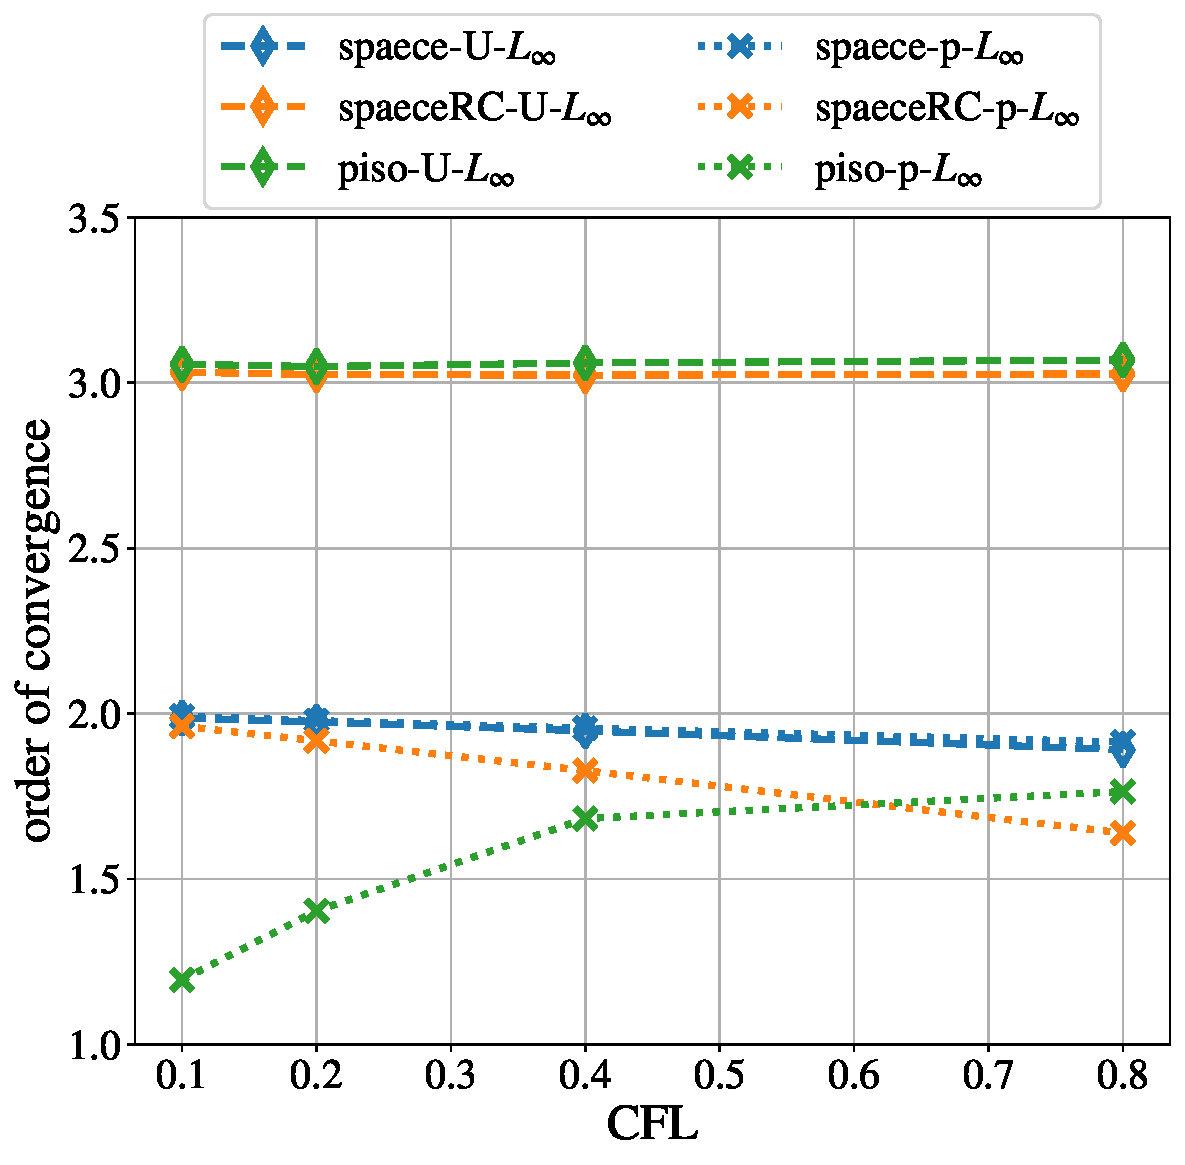
\includegraphics[width=\imgHalfWidth\columnwidth]{TGV2D/Re1000/Cartesian/ErrorNormComp_Inf.pdf}\label{fig:TGV2D-Cart1000-CFL-inf}} 
\caption{Order of convergence comparison for across CFL numbers for \spaece, \spaeceRC and \piso algorithms in Cartesian square mesh} 
\label{fig:TGV2D-Cart1000-CFL}
\end{figure}

The isolated temporal and spatial error order of convergence are important indicators of any algorithm. However in practice, fluid flow problems are often solved at a certain CFL number\cite{courant1928, courant1967} limit and in such cases, the mixed order of convergence is also import to the user. 2D Taylor-Green vortex at $Re\, 1\times10^3$ is simulated in four Cartesian square meshes: $33 \times 33$, $65 \times 65$, $127 \times 127$ and $257 \times 257$. Times steps are adjusted for each mesh to simulate the cases in a series of four CFL numbers: $0.1, \, 0.2,\, 0.4$ and $0.8$. The order of convergence for the \spaece, \spaeceRC and \piso algorithms are reported in Fig. \ref{fig:TGV2D-Cart1000-CFL}. 
%(i.e. $4\times 4 = 16$ simulations)

The \spaece algorithm demonstrated 2nd order error convergence for both velocity and pressure fields with slight decrease at high CFL numbers. Application of  Rhie-Chow correction increased velocity error convergence rate to 3rd order for both \spaeceRC and \piso algorithms. The \spaeceRC algorithm delivered 2nd order error convergence for pressure at CFL $0.1$ and proportionally decreased to 1.58th order for CFL $0.8$. On the other hand, the \piso algorithm achieved 1.2th order of convergence for pressure, which gradually increased to 1.75th order at CFL $0.8$. 
Overall, at $CFL < 0.5 $ the \spaeceRC delivers better pressure error convergence and at $CFL > 0.5$ both of the \spaeceRC and \piso algorithms provide similar near 2nd order error convergence.


%\clearpage
\subsubsection{Order of convergence in non-orthogonal mesh}
Non-orthogonality can bring significant change in order of convergence of any algorithm. The laminar 2D Taylor-Green vortex ($Re\, 1\times10^3$) is simulated in a series of mesh where each square is split into two right-angle triangles (i.e. each triangle has two non-orthogonal faces). Thus, any Cartesian square $N \times N$ mesh is converted into right-angle triangulated $(N \times N) \times 2$ mesh.

\begin{figure}[!h]
\centering
\subfloat[$L_2$ error norm]{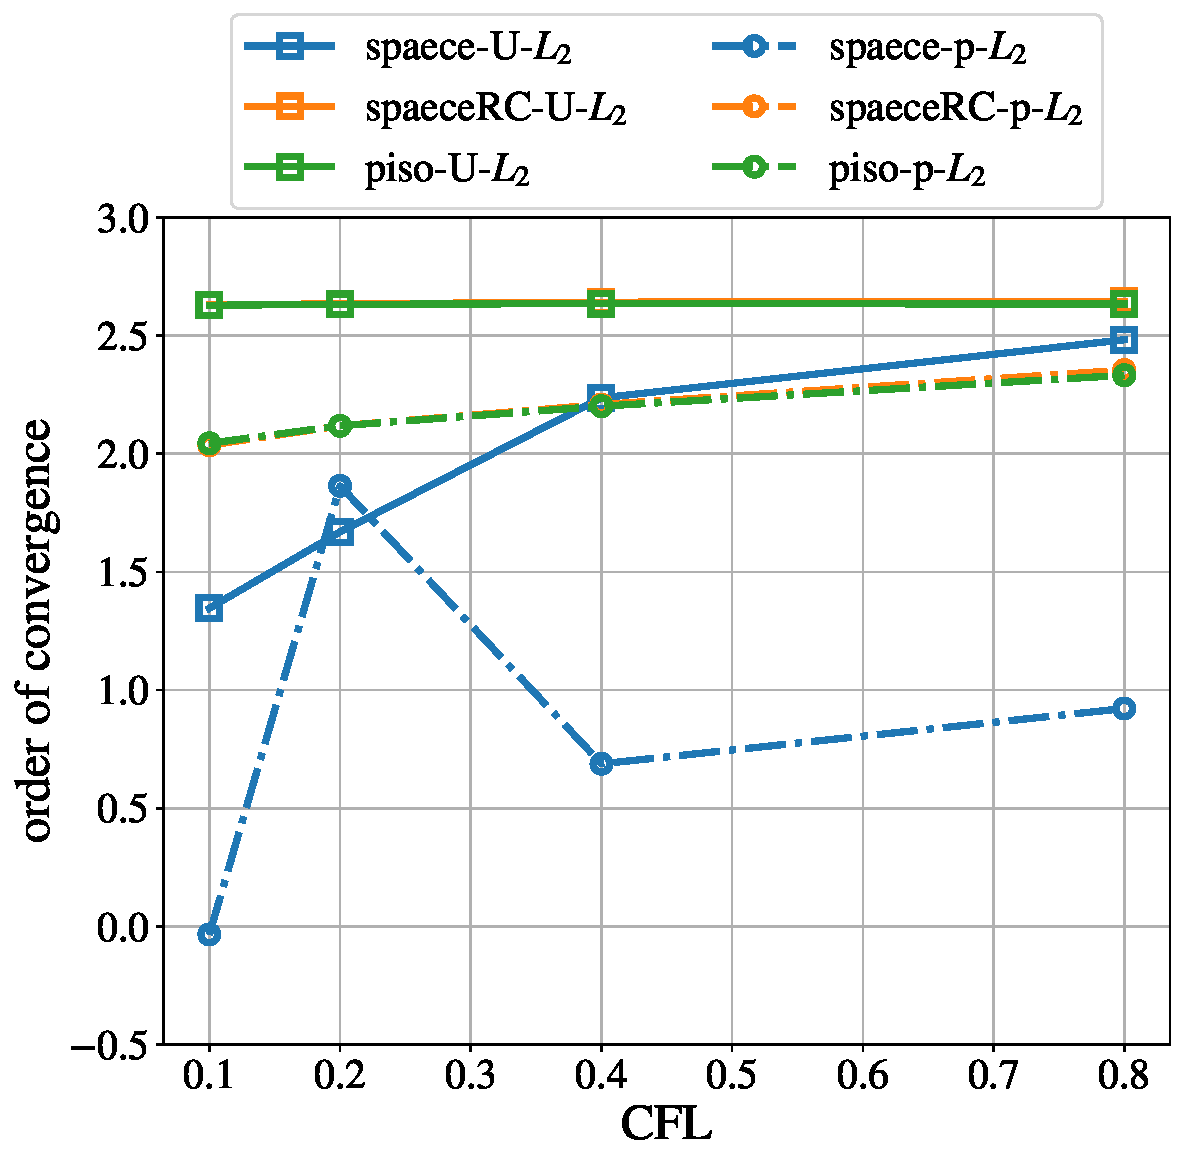
\includegraphics[width=\imgHalfWidth\columnwidth]{TGV2D/Re1000/rightAnglePrism/ErrorNormComp_2nd.pdf}\label{fig:TGV2D-RAT1000-CFL-2nd}}
\subfloat[$L_\infty$ error norm]{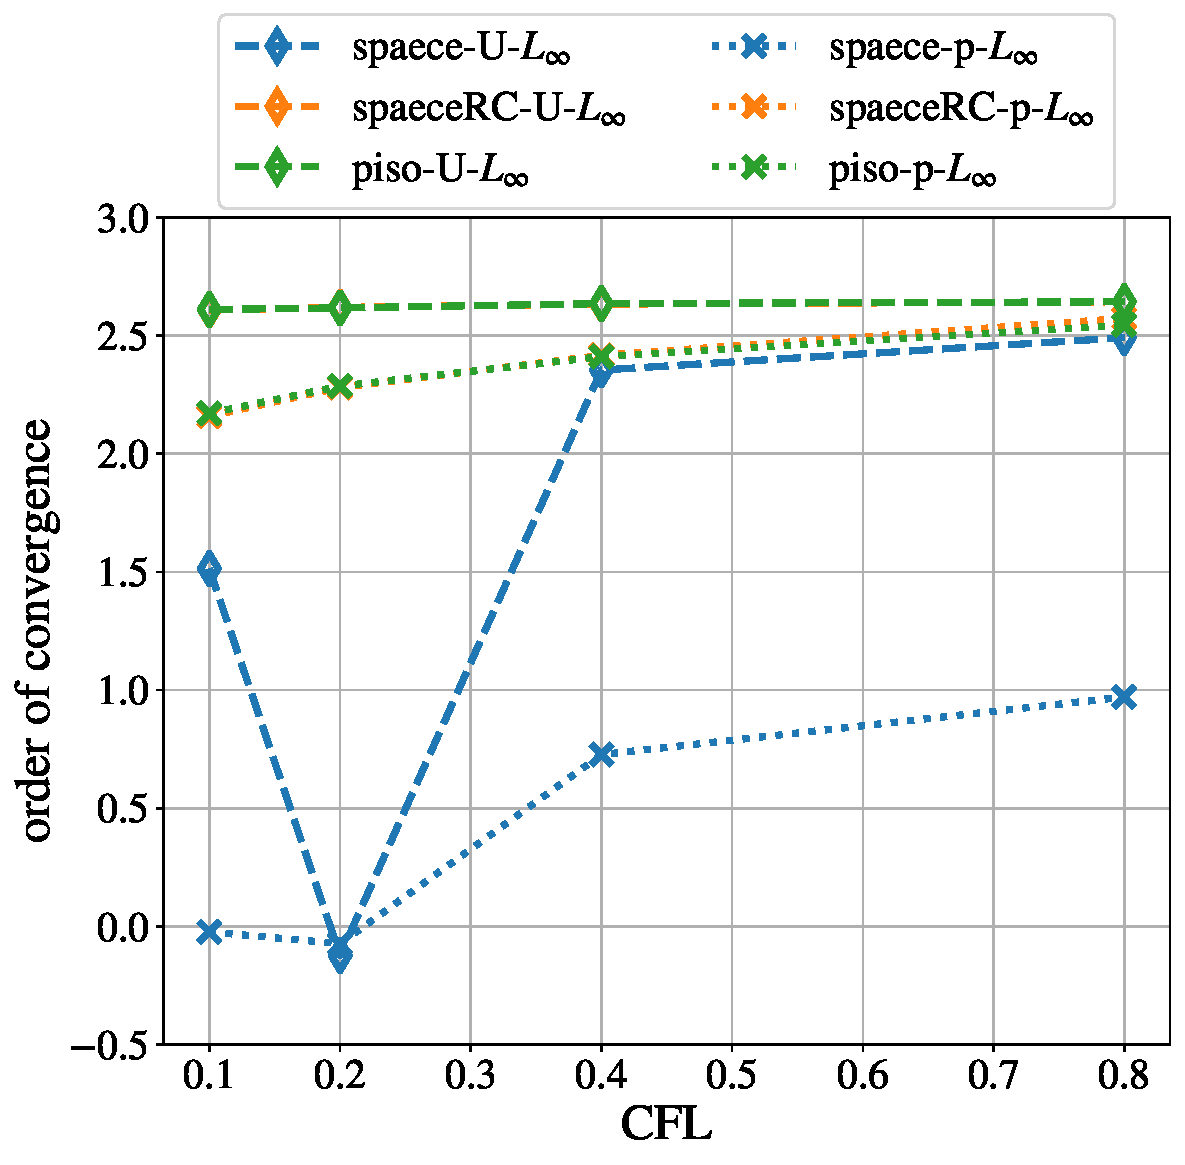
\includegraphics[width=\imgHalfWidth\columnwidth]{TGV2D/Re1000/rightAnglePrism/ErrorNormComp_Inf.pdf}\label{fig:TGV2D-RAT1000-CFL-inf}} 
\caption{Order of convergence comparison for across CFL numbers for \spaece, \spaeceRC and \piso algorithms in right-angle triangulated mesh} 
\label{fig:TGV2D-RAT1000-CFL}
\end{figure}

Similar to the study on Cartesian square meshes (Sec. \ref{sec:OoC-RC}), the order of error convergence across multiple CFL numbers for right-angle triangulated meshes is reported in Fig. \ref{fig:TGV2D-RAT1000-CFL}. The \spaece algorithm provided inconsistent order of convergence, emphasizing the importance of Rhie-Chow correction. The \spaeceRC and \piso algorithms both provided near-identical results. When compared to the Cartesian square mesh results, the order of convergence for velocity errors dropped from 3rd order to 2.6th order, and the pressure errors are slightly increased above 2nd order. 

%\clearpage
%\newpage
\subsection{Minimize artificial dissipation}
\label{sec:minimizeArtificialDissipation}
In accordance with KE conservation for inviscid flow (Sec. \ref{sec:inviscidKE}), there shall not be any artificial dissipation in a viscous flow simulation, i.e. the molecular and turbulence dissipative terms shall be the sole source KE decay. 

A LES of 3D Taylor-Green vortex with $Re = 5\times10^3$ is simulated with the \spaece algorithm for a Cartesian cubic $65 \times 65 \times 65$ mesh and a right-angle prism $(65 \times 65) \times 2 \times 65$ mesh. To model the sub-filter scales, the dynamic k equation turbulence model (cite Heinz) is used with the polyLaplace filter (Eq. \eqref{eqn:polyLaplace}) coefficient $\epsilon = 2$ and grid-spacing coefficient $\Delta =1$. Fig. \ref{fig:TGV3Dcomp-k} highlights the difference in KE decay between the Cartesian (orthogonal) mesh and the right-angle prism (non-orthogonal) mesh. In Fig. \ref{fig:TGV3Dcomp-eps}, the KE decay rate exactly matches the dissipation rate induced by total viscosity $\nu_{eff}$. 

\begin{figure}[!h]
\centering
\subfloat[KE decay]{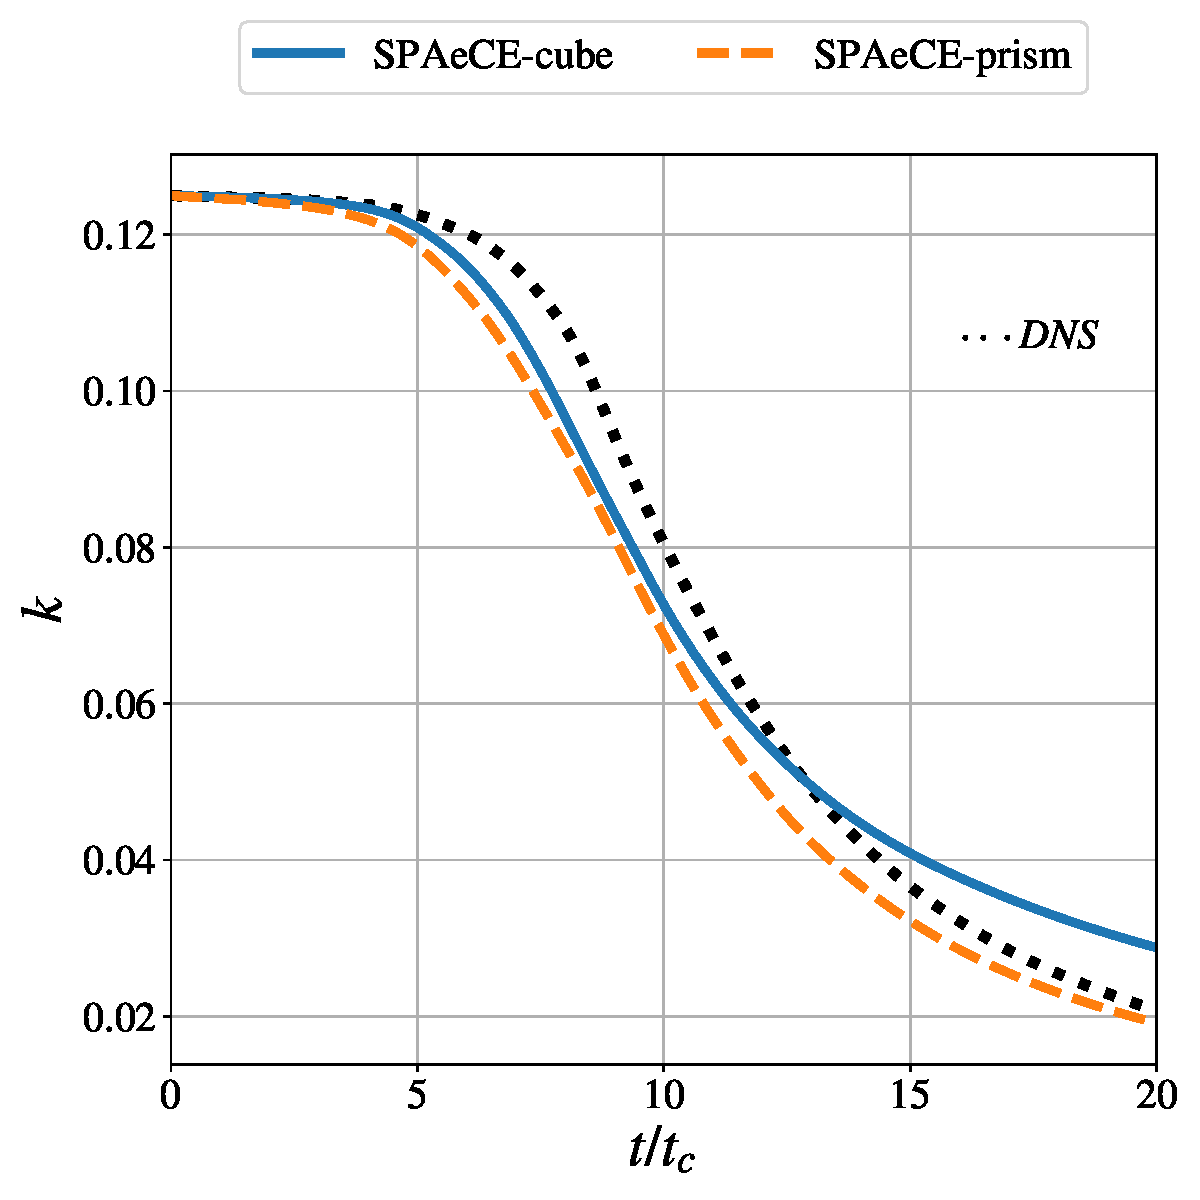
\includegraphics[width=\imgHalfWidth\columnwidth]{TGV3D/Re5000/spaeceFoamCNTGV/cubeVsPrism/65cubed/3DTGV_Re5000_spaeceFoamCNTGV_dynKEqnHeinz_8x8_k.pdf}\label{fig:TGV3Dcomp-k}}
\subfloat[KE decay rate \& dissipation rate]{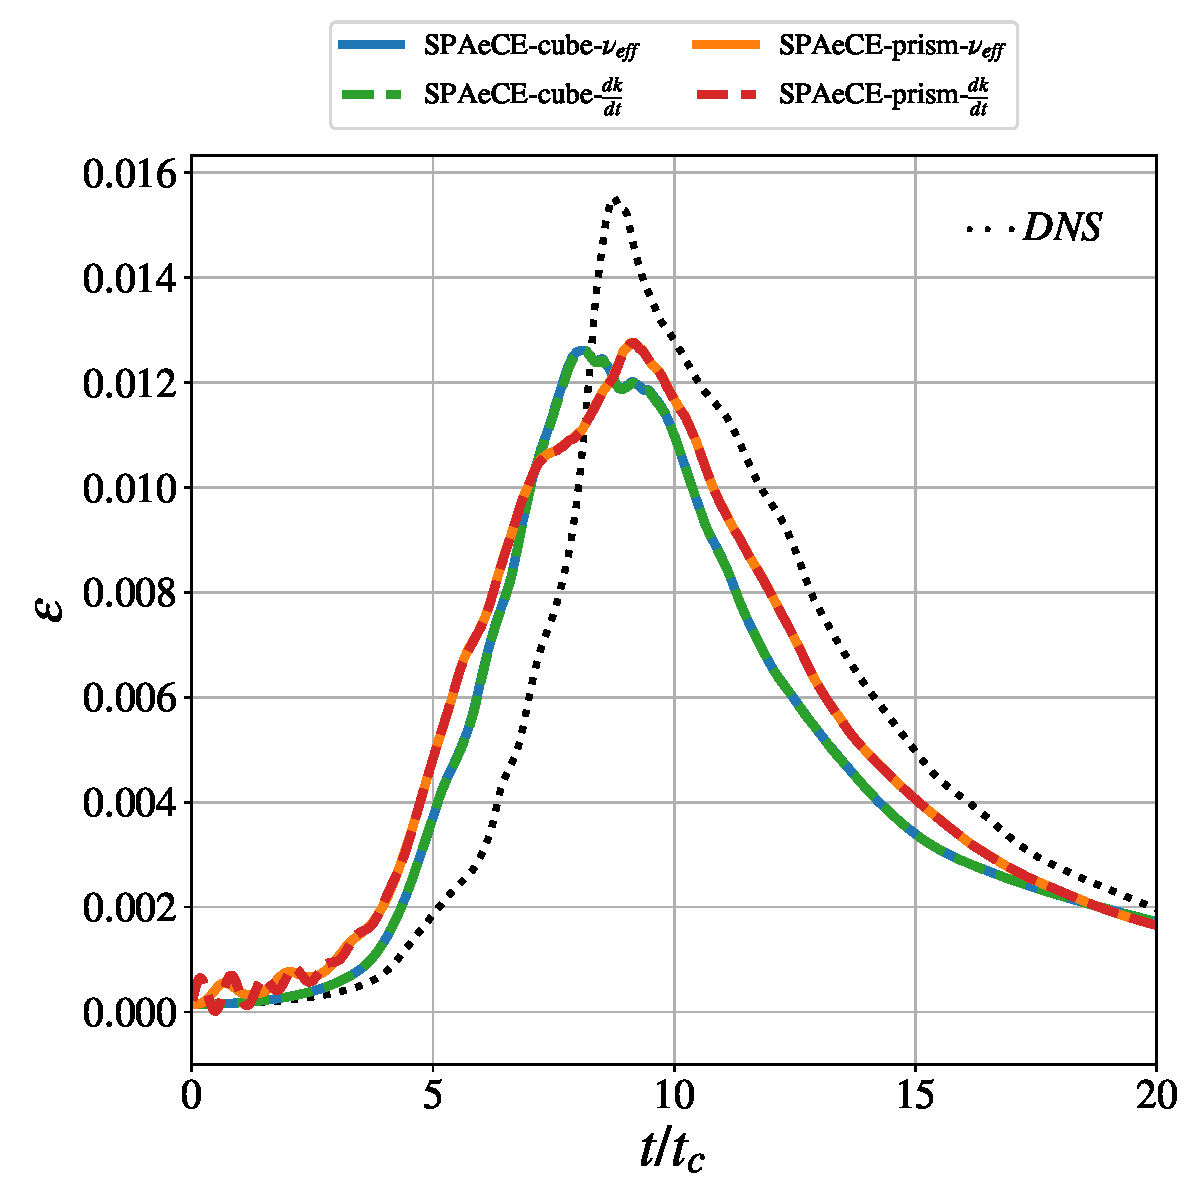
\includegraphics[width=\imgHalfWidth\columnwidth]{TGV3D/Re5000/spaeceFoamCNTGV/cubeVsPrism/65cubed/3DTGV_Re5000_spaeceFoamCNTGV_dynKEqnHeinz_8x8_epsDkdt0.pdf}\label{fig:TGV3Dcomp-eps}} 
\caption{Comparison of \spaece algorithm KE decay (left), and KE decay rate and dissipation rate (right) in a 3D Taylor-Green vortex of $Re = 5\times10^3$ between a Cartesian cubic $65 \times 65 \times 65$ mesh and a right-angle prism $(65 \times 65) \times 2 \times 65$ mesh} 
\label{fig:TGV3Dcomp}
\end{figure}

In the right-angle prism mesh, the early oscillatory nature of the KE decay rate and dissipation rate (see Fig. \ref{fig:TGV3Dcomp-eps}) is due to the presence of strong checker-board like pattern, which results in increased dissipation and eventually, affected the KE evolution at all subsequent times. Overall, the \spaece algorithm produces no artificial dissipation in both orthogonal and non-orthogonal meshes, but the influence of mesh types remain.



%\clearpage
%\newpage
\subsection{Damping the high frequency modes}
\label{sec:dampHFModes}

In Sec. \ref{sec:advReg}, we have mentioned that $A6$ regularization when applied to the \spaece algorithm does not add any artificial dissipation. In Fig. \ref{fig:TGV3D-5k-A6} influence of $A6$ regularization in a 3D Taylor-Green vortex with $Re = 5 \time 10^3$ simulated in Cartesian cubic $65 \times 65 \times 65$ and $129 \times 129 \times 129$ mesh.

To model the sub-filter scales in the \spaece solver, the dynamic k equation turbulence model (cite Heinz) is used with the polyLaplace filter (Eq. \eqref{eqn:polyLaplace}) coefficient $\epsilon = 2$ and grid-spacing coefficient $\Delta =1$.  For the \spaeceA solver, the polyLaplace residual-filter (Eq. \eqref{eqn:resFilter}) with $\epsilon = 3,\,\Delta =1$ is used for regularization. Since the $A6$ method dampens the near-filter high frequency modes, the grid-spacing coefficient is raised to $\Delta =1.5$ and filter coefficient retained at $\epsilon = 2$ for SFS polyLaplace filter. There are slight difference in KE decay rate between the \spaece and \spaeceA algorithms, however in both meshes KE decay rate exactly matches with the total dissipation.

\begin{figure}[!h]
\centering
\subfloat[$65 \times 65 \times 65$ mesh]{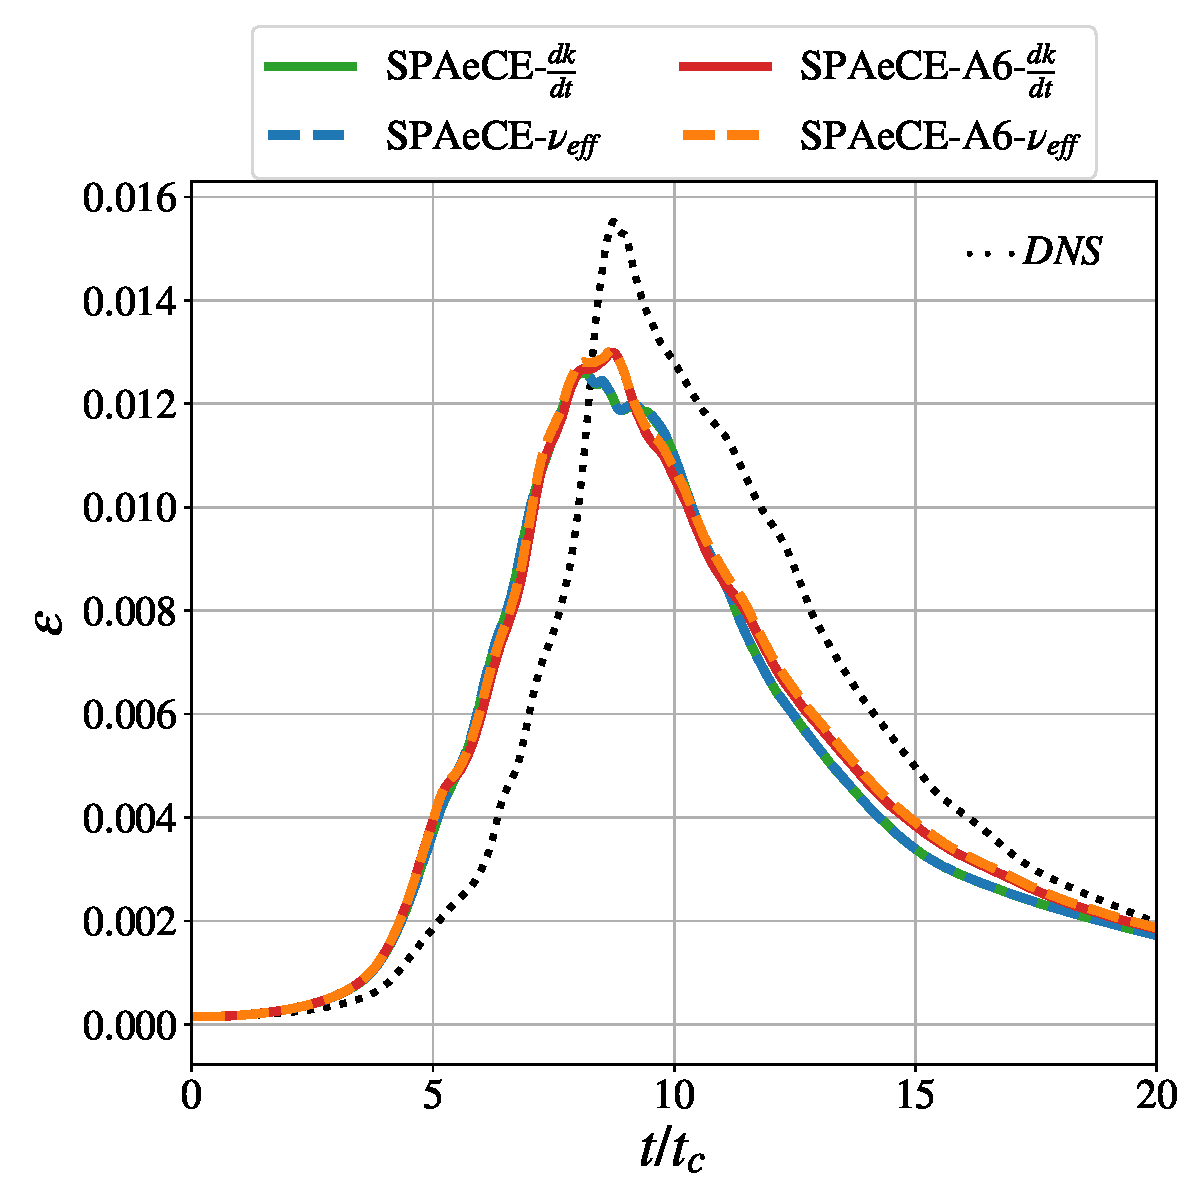
\includegraphics[width=\imgHalfWidth\columnwidth]{TGV3D/Re5000/spaeceFoamCNTGV/spaeceVsSpaeceA6/65x65x65/3DTGV_Re5000_spaeceFoamCNTGV_dynKEqnHeinz_8x8_epsDkdt0.pdf}\label{fig:TGV3D-5k-A6-65}}
\subfloat[$129 \times 129 \times 129$ mesh]{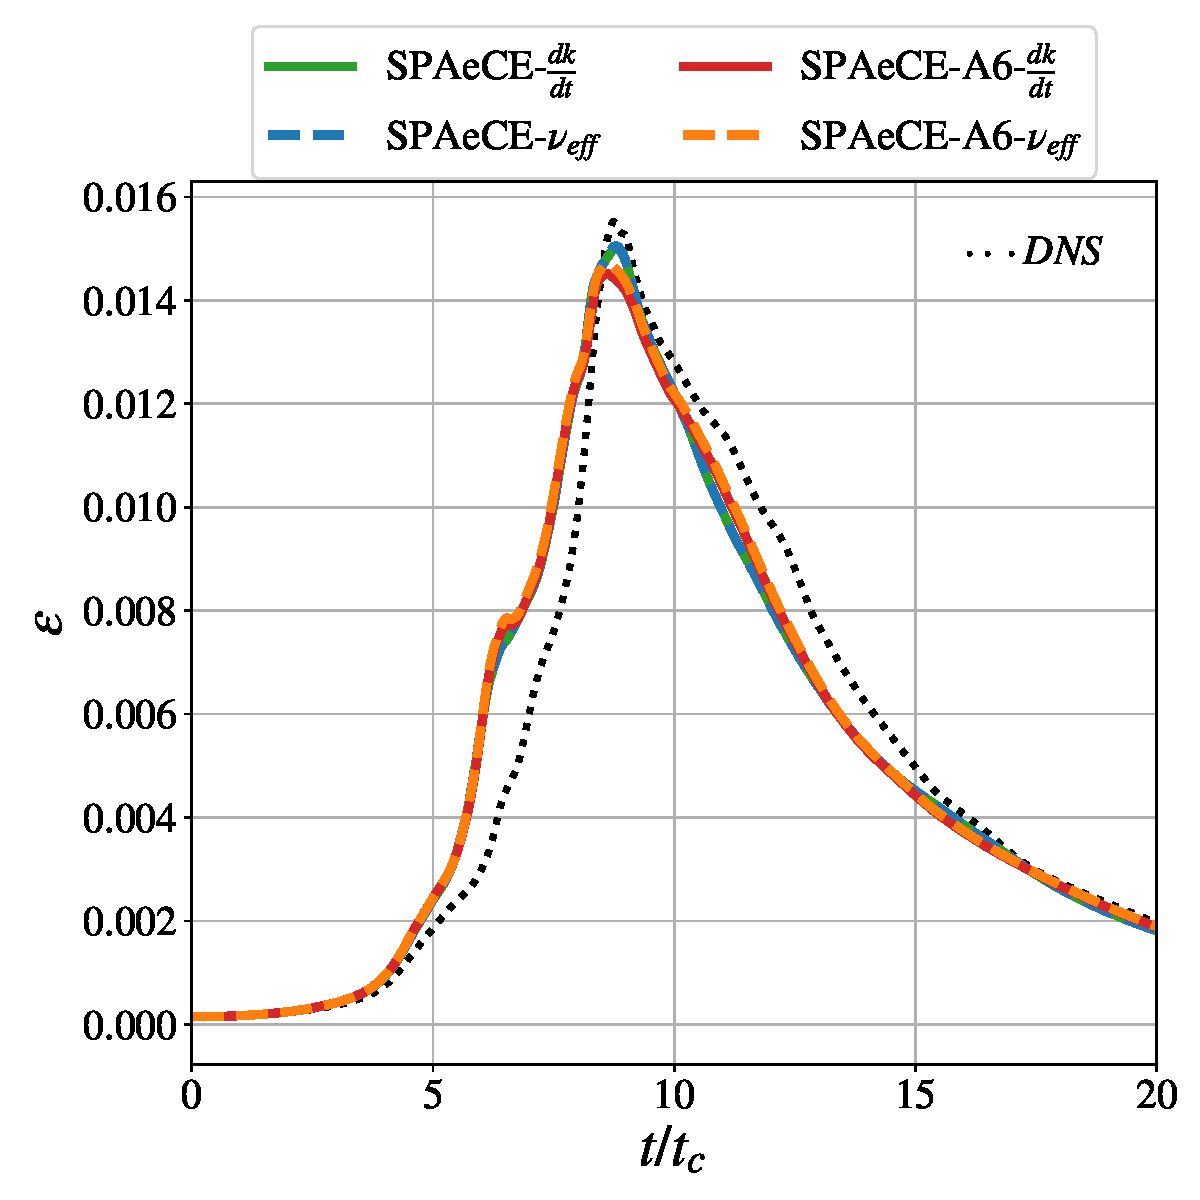
\includegraphics[width=\imgHalfWidth\columnwidth]{TGV3D/Re5000/spaeceFoamCNTGV/spaeceVsSpaeceA6/129x129x129/3DTGV_Re5000_spaeceFoamCNTGV_dynKEqnHeinz_8x8_epsDkdt0.pdf}\label{fig:TGV3D-5k-A6-129}} 
\caption{$A6$ regularization does not add any dissipation} 
\label{fig:TGV3D-5k-A6}
\end{figure}

In addition to an artificial dissipation free regularization, the $A6$ advection regularization method redistributes energy from the near-filter-cutoff $\kappa_{cutoff}$, high frequency modes to the lower frequency modes by dissipating the high frequency modes faster than the inertial range cascade. 

To investigate influence of the $A6$ regularization, KE spectrum for the 3D Taylor-Green vortex at time $t/t_c =9$ is compared at Fig. \ref{fig:TGV3D-5k-A6Spec}. The \spaece algorithm demonstrated a constant slope at the inertial range. In case of the \spaeceA algorithm, the slope of the energy cascade gets steeper roughly from $k_{cutoff}/2$ to $k_{cutoff}$ wave-numbers. For the fine $129 \times 129 \times 129$ mesh, the \spaeceA algorithm successfully attenuated the high-frequency modes and obtained a better match with the KE spectrum.

\begin{figure}[!h]
\centering
\subfloat[$65 \times 65 \times 65$ mesh]{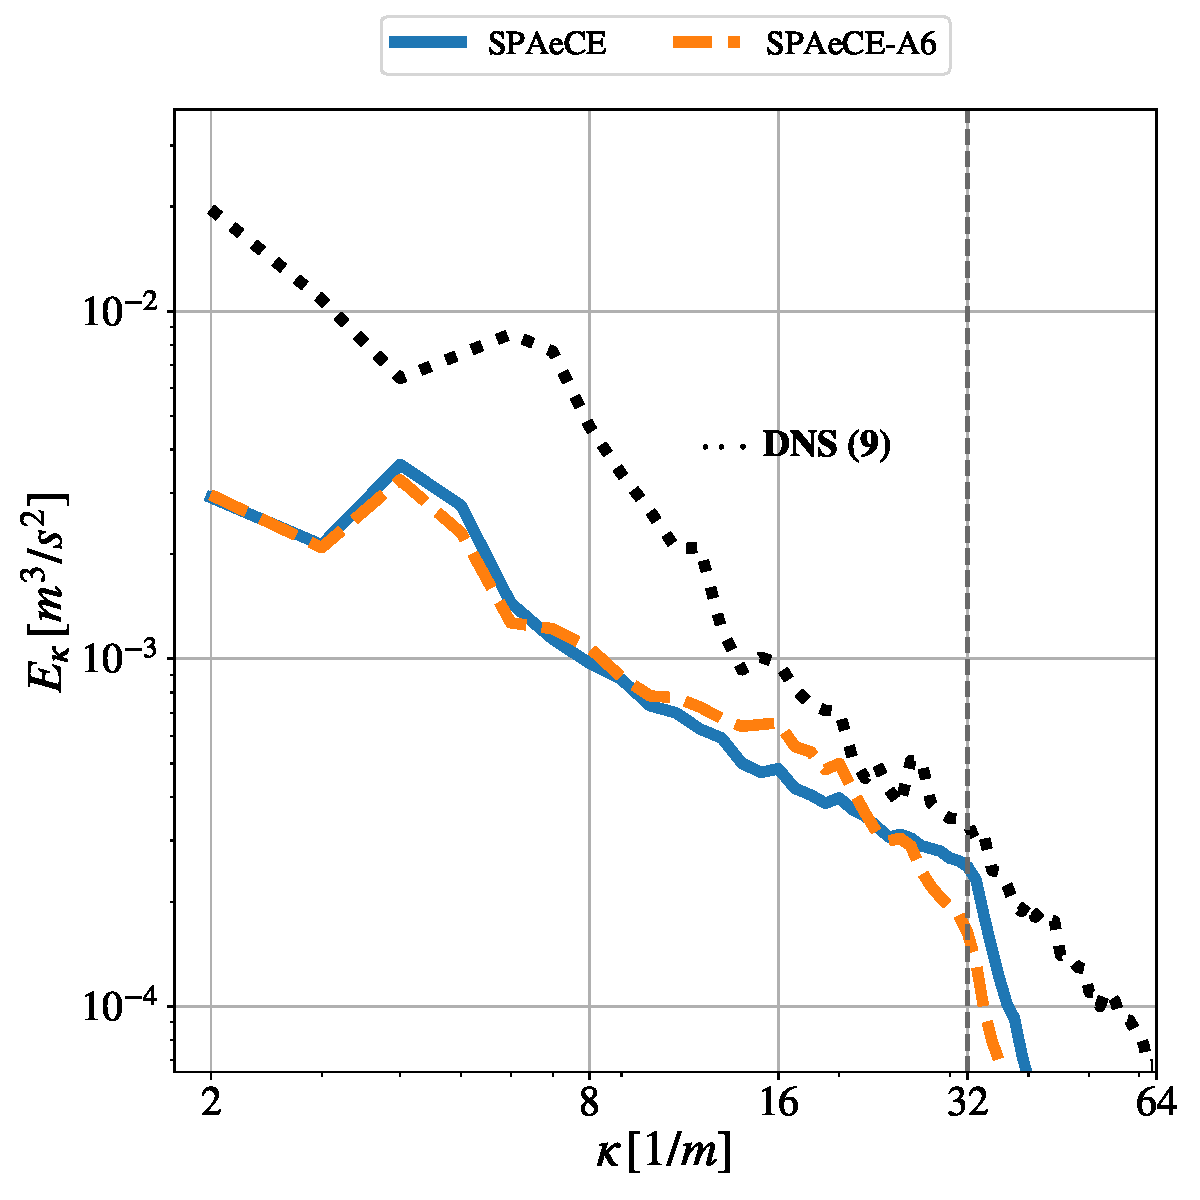
\includegraphics[width=\imgHalfWidth\columnwidth]{TGV3D/Re5000/spaeceVsSpaeceA6/65x65x65/spectrum/3DTGV5000-energySpectrum-dynKEqnHeinz-Time090.pdf}\label{fig:TGV3D-5k-A6Spec-65}}
\subfloat[$129 \times 129 \times 129$ mesh]{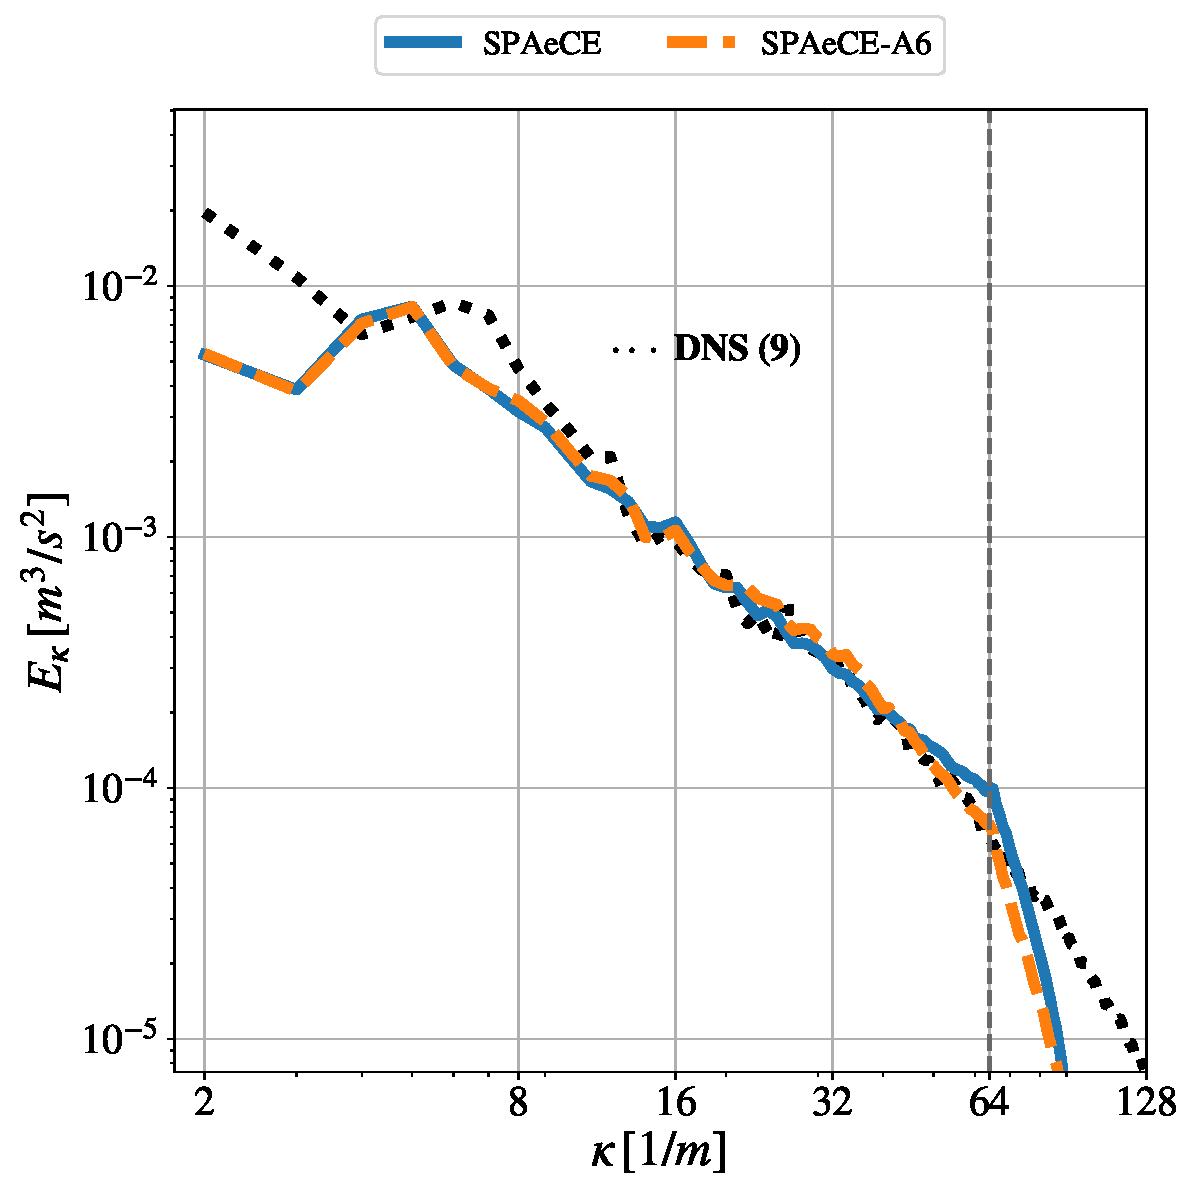
\includegraphics[width=\imgHalfWidth\columnwidth]{TGV3D/Re5000/spaeceVsSpaeceA6/129x129x129//spectrum/3DTGV5000-energySpectrum-dynKEqnHeinz-Time090.pdf}\label{fig:TGV3D-5k-A6Spec-129}} 
\caption{$A6$ dampens the high frequency modes} 
\label{fig:TGV3D-5k-A6Spec}
\end{figure}

Besides the 3D Taylor-Green vortex case, decay of an incompressible homogeneous isotropic turbulence case is also simulated following the experimental investigation performed by Comte-Bellot and Corrsin \cite{CBC1971}. Flow field measurements were performed at $Re = 3.4\times10^4$ with characteristic velocity (free-stream) $U_0 = 10\, m/s$ and characteristic length-scale (grid-spacing) $M = 5.08\, cm$ (or $2$ inch). Thus the molecular viscosity is $ \nu = \frac{U_0 M}{Re} = \frac{10 \times 0.0508}{3.4\times10^4} = 1.49412 \times10^{-4} \approx 1.5\times10^{-4} m^2/s$. In the reference experiment, turbulence kinetic energy (TKE) spectrum is computed at non-dimensional times of $t_c = \frac{U_0 t}{M} = 42,\, 98$ and $171$; equating to dimensional times of $0.213s,\, 0.498s$ and $0.869s$ respectively.

The computational domain comprises a 3D cube with side length of $9\times2\pi\, cm$. Initial turbulent velocity field at time $0.213s$ is generated using the OpenFOAM-v1912 \emph{createBoxTurb}\footnote{The createBoxTurb application implements the synthetic turbulence generation method proposed by Saad et al. \cite{Saad2016}; open source code available at: https://www.openfoam.com/documentation/guides/latest/man/createBoxTurb.html} utility following the corresponding turbulence kinetic energy spectrum reported by Comte-Bellot and Corrsin \cite[Table 3]{CBC1971}. The sub-filter stress in the \spaece and \spaeceA algorithms are modeled following the same approach as the 3D Taylor-Green vortex case. Finally, the Turbulence Kinetic Energy (TKE) spectrum is compared at times $t_c =98\, (t=0.498s)$ and $t_c =171\, (t=0.869s)$ (Fig. \ref{fig:HIT98}).

\begin{figure}[!h]
\centering
\subfloat[$65 \times 65 \times 65$]{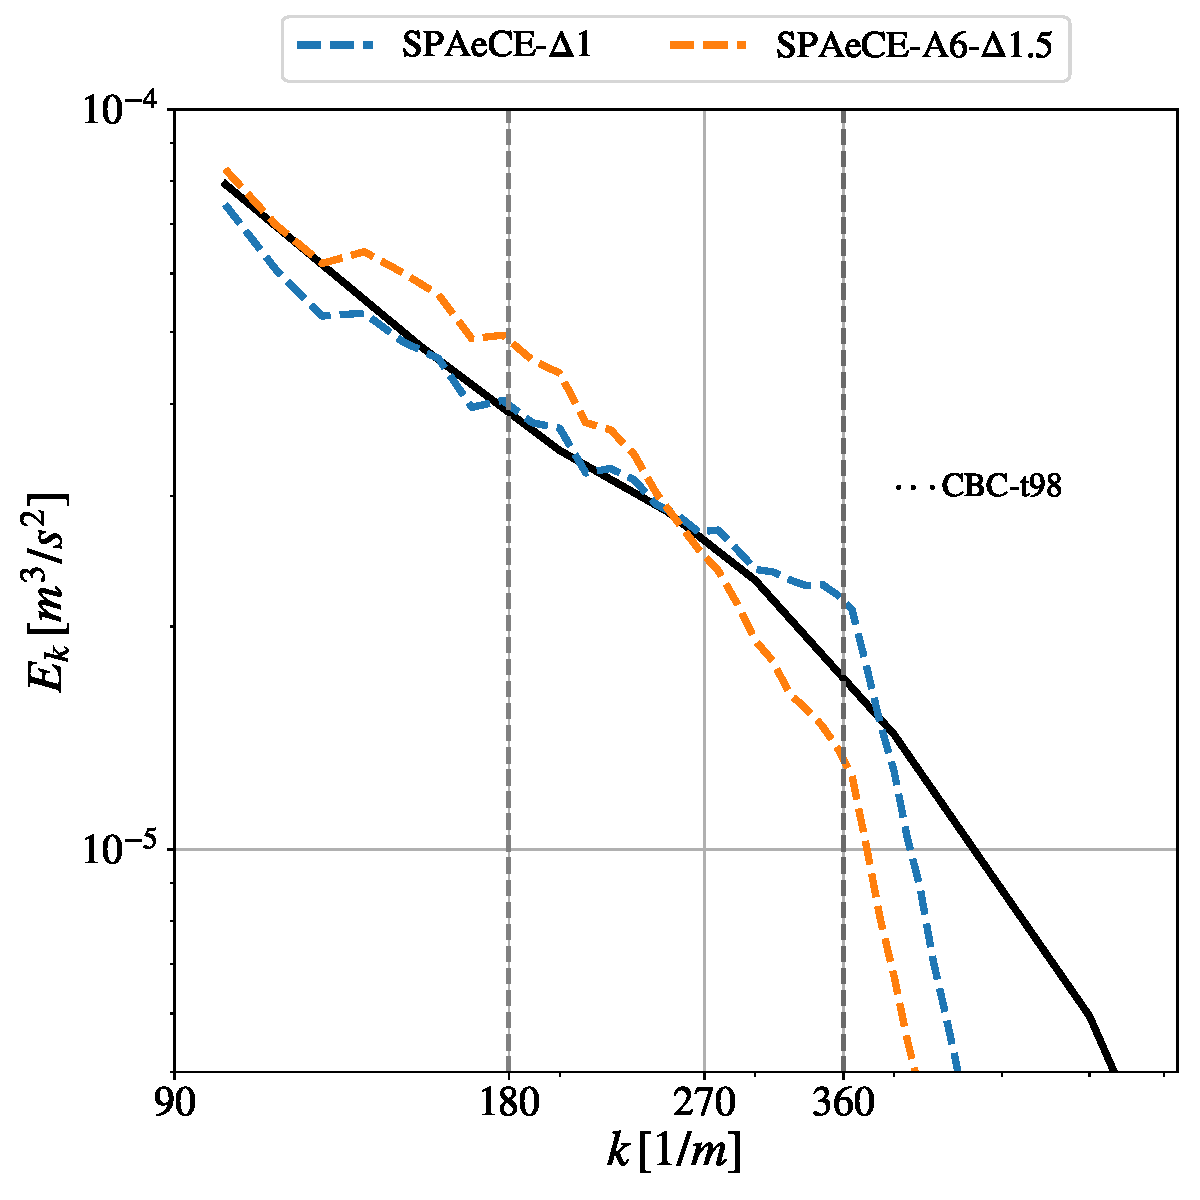
\includegraphics[width=\imgHalfWidth\columnwidth]{HITCBC/65cubed/HIT-energySpectrum-Zoomed-Time98.pdf}\label{fig:HIT98-65}}
\subfloat[$129 \times 129 \times 129$]{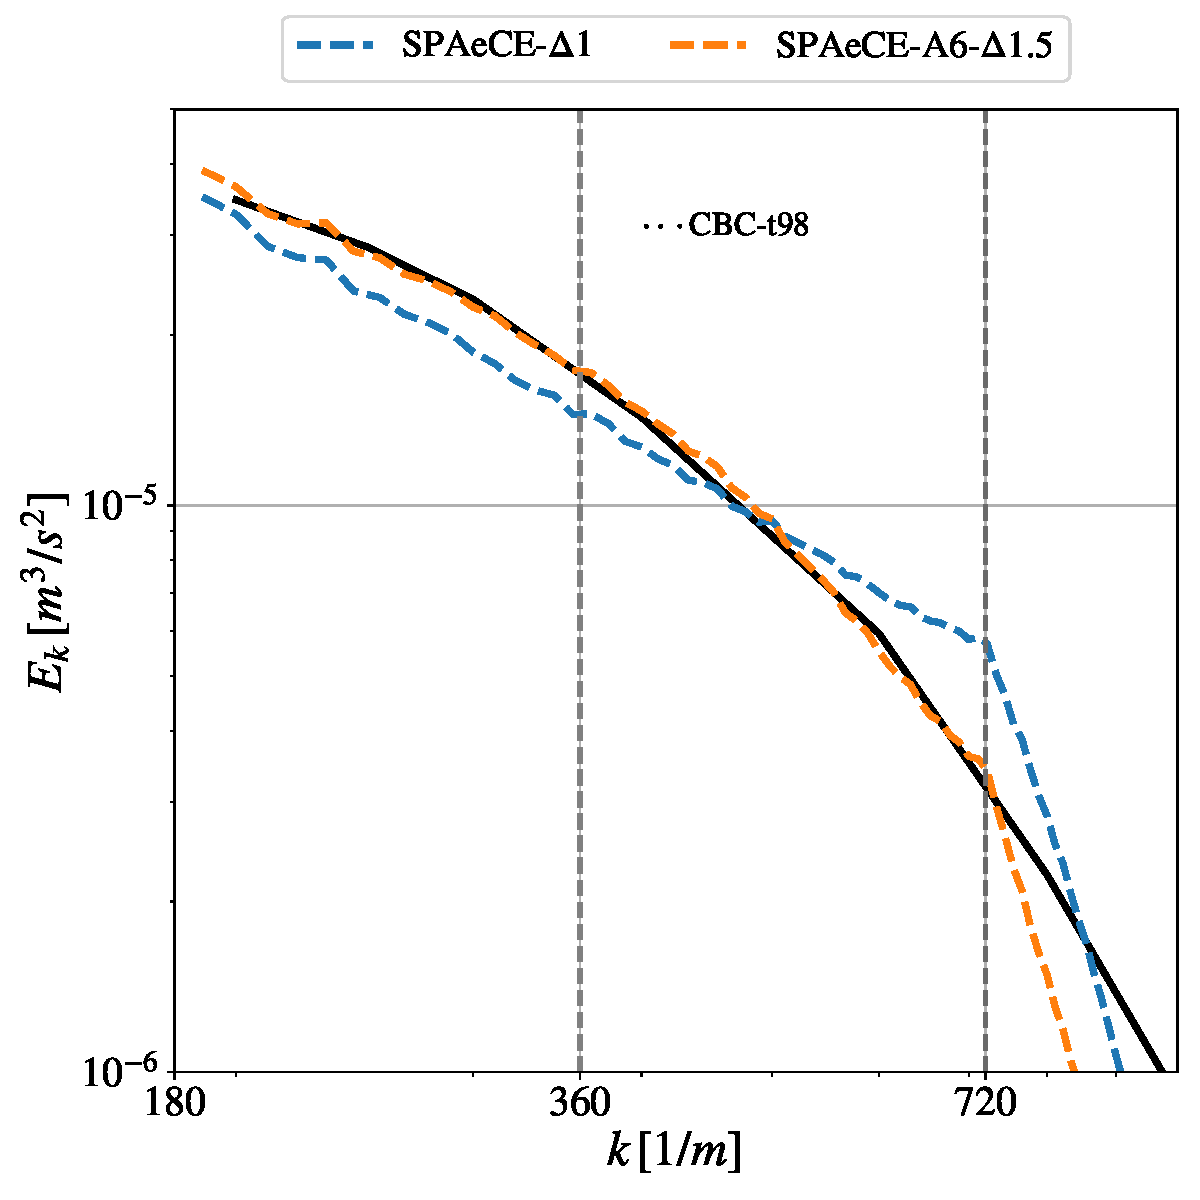
\includegraphics[width=\imgHalfWidth\columnwidth]{HITCBC/129cubed/HIT-energySpectrum-Zoomed-Time98.pdf}\label{fig:HIT98-129}} 
\caption{Homogeneous isotropic turbulence } 
\label{fig:HIT98}
\end{figure}

%Introduce A6 correction: show results from HIT-CBC and 3D TGV Re 5000 cases.

In both test cases, the \spaeceA solver achieved significant improvement in KE spectrum match over the \spaece solver in the well resolved $129 \times 129 \times 129$ mesh (Fig. \ref{fig:HIT98-129}). However, for the coarse $65 \times 65 \times 65$ mesh, the $A6$ regularization seems to over dampen the near filter modes and energy accumulation is observed in the intermediate range(Fig. \ref{fig:HIT98-65}). Thus, use of $A6$ regularization to coarsely resolved mesh is not recommended!

Application of the $A6$ regularization in conjunction with Rhie-Chow correction deliver better results that application of Rhie-Chow correction alone! In the 3D Taylor-Green vortex of $Re = 5 \times 10^3$ simulation with Cartesian cubic mesh, \spaeceARC algorithm has less artificial dissipation (see Fig. \ref{fig:TGV3D-5k-A6RC}) and better spectrum match (see Fig. \ref{fig:TGV3dSpec}) compared to the \spaeceRC algorithm. The superiority of the \spaeceARC algorithm is more prominent in the coarse $65 \times 65 \times 65$ mesh than the fine $129 \times 129 \times 129$ mesh. The \piso algorithm displayed most non-physical dissipation and least spectrum match for both meshes. Therefore, \spaeceARC is our recommended algorithm, although the $A6$ regularization may increase the computational time to approximately $10 \%$ compared to the \spaeceRC algorithm.

% The $A6$ regularization redistributes energy from the high frequency modes to intermediate frequency modes, thus leaving less energy at high-frequecy modes which are most affection by the Rhie-Chow correction. In absence any regularization, the Rhie-Chow correction dissipates lot more energy, thus larger non-physical dissipation. % doulble check if its the implicit convection term and advection regularization?%

\begin{figure}[!h]
\centering
\subfloat[$65 \times 65 \times 65$ mesh]{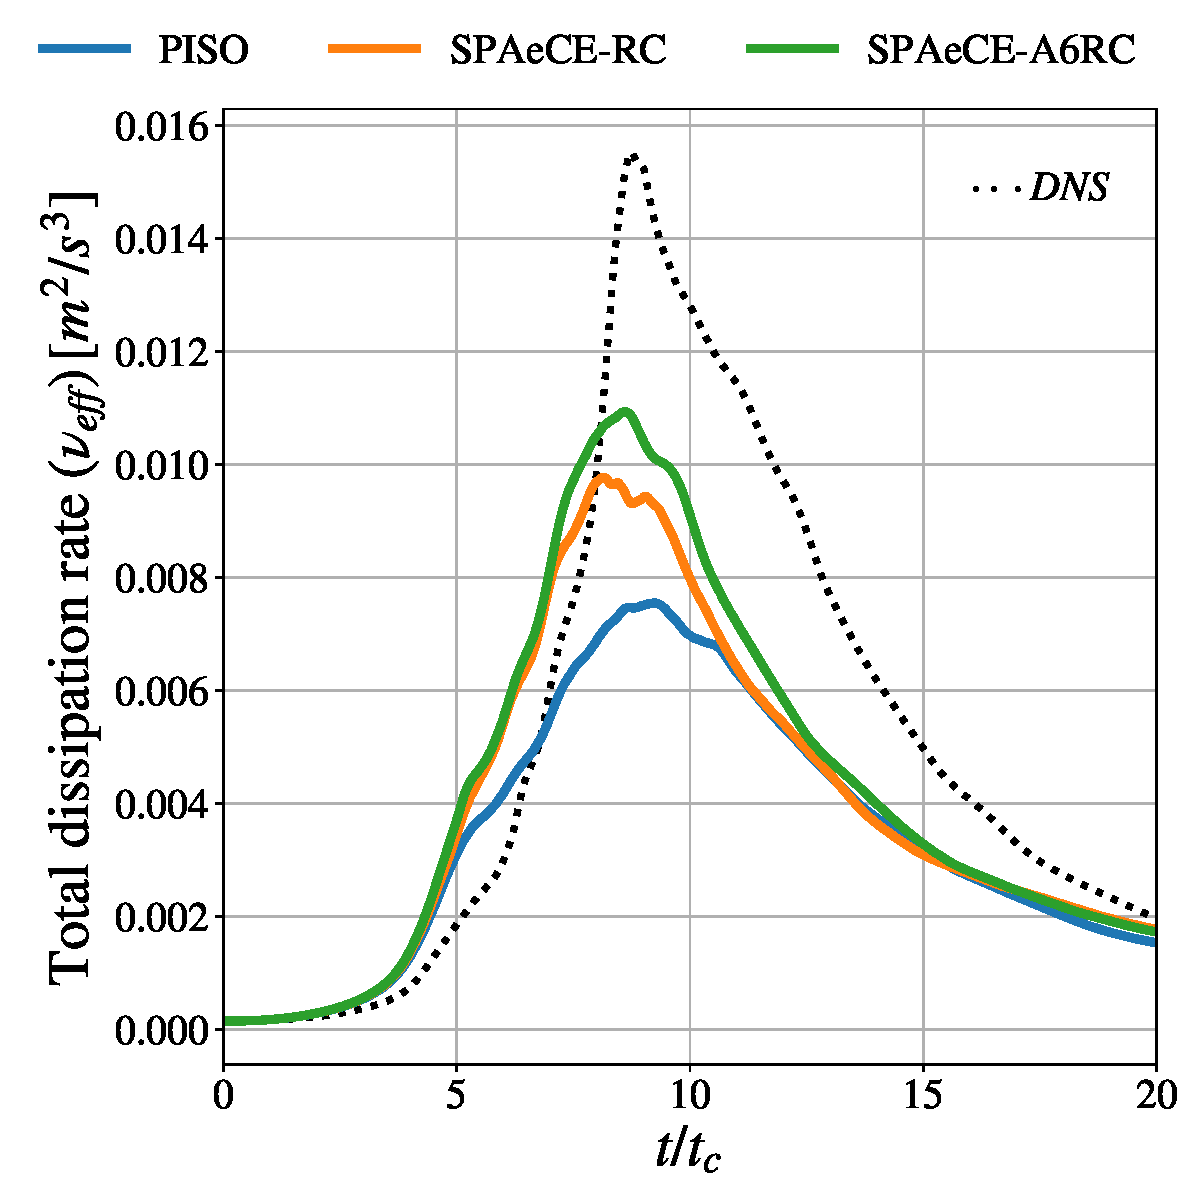
\includegraphics[width=\imgHalfWidth\columnwidth]{TGV3D/Re5000/pisoVsSpaeceRCVsSpaeceA6RC/65x65x65/3DTGV_Re5000_dynKEqnHeinz_8x8_nuEff.pdf}\label{fig:TGV3D-5k-A6RC-65}}
\subfloat[$129 \times 129 \times 129$ mesh]{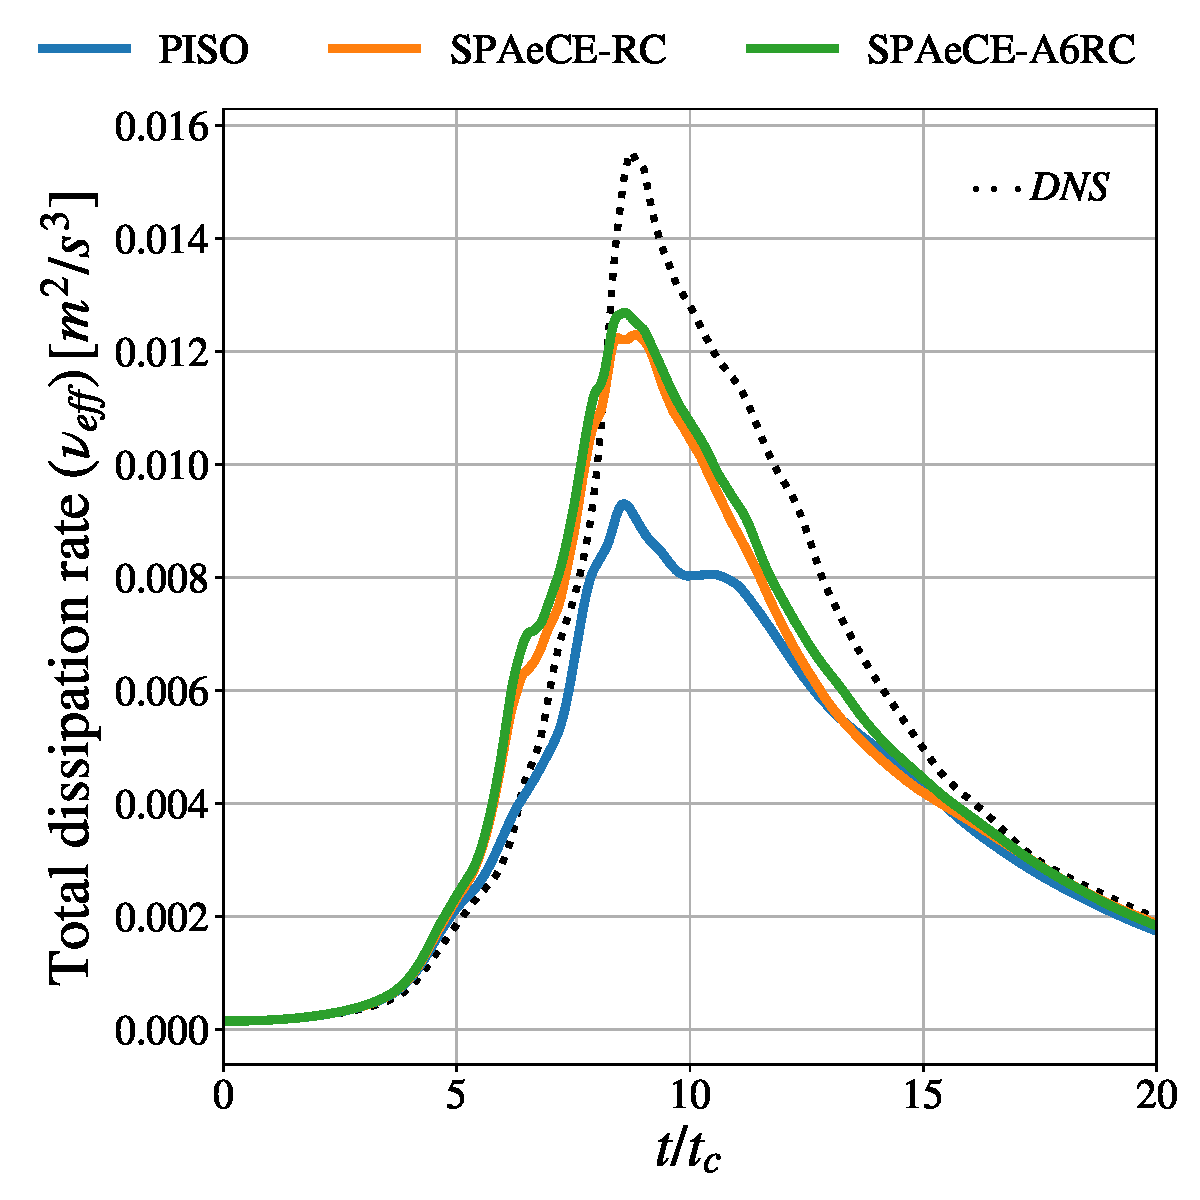
\includegraphics[width=\imgHalfWidth\columnwidth]{TGV3D/Re5000//pisoVsSpaeceRCVsSpaeceA6RC/129x129x129/3DTGV_Re5000_dynKEqnHeinz_8x8_nuEff.pdf}\label{fig:TGV3D-5k-A6EC-129}} 
\caption{$A6RC$ regularization better than RC} 
\label{fig:TGV3D-5k-A6RC}
\end{figure}


\begin{figure}[!h]
\centering
\subfloat[$65 \times 65 \times 65$]{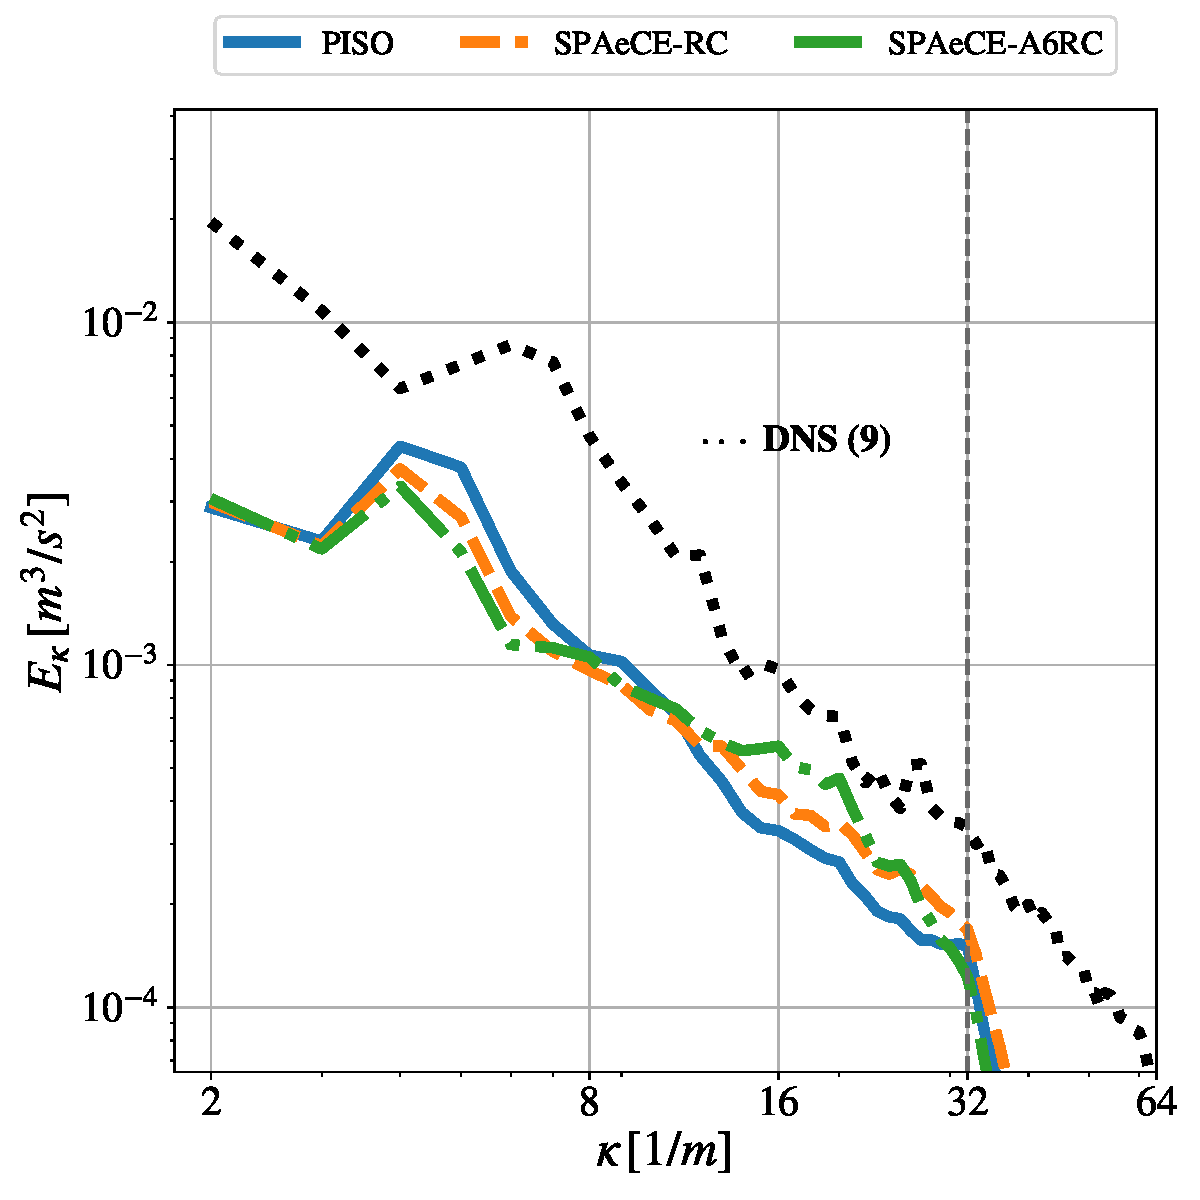
\includegraphics[width=\imgHalfWidth\columnwidth]{TGV3D/Re5000/pisoVsSpaeceRCVsSpaeceA6RC/65x65x65/spectrum/3DTGV5000-energySpectrum-dynKEqnHeinz-Time090.pdf}\label{fig:TGV3dSpec-65}}
\subfloat[$129 \times 129 \times 129$ mesh]{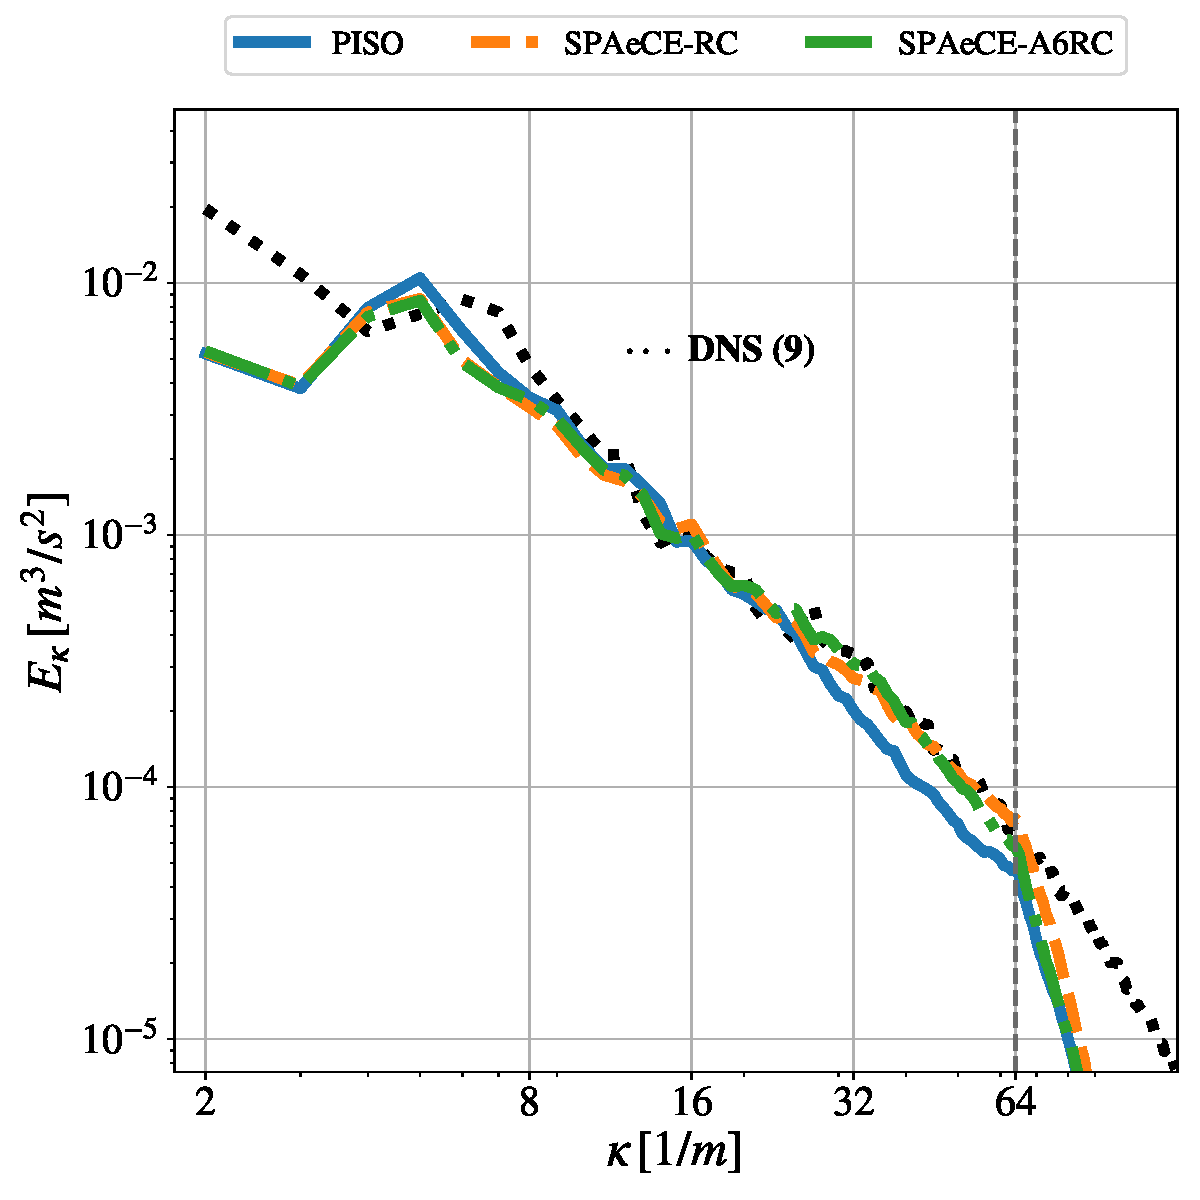
\includegraphics[width=\imgHalfWidth\columnwidth]{TGV3D/Re5000/pisoVsSpaeceRCVsSpaeceA6RC/129x129x129/spectrum/3DTGV5000-energySpectrum-dynKEqnHeinz-Time090.pdf}\label{fig:TGV3dSpec-129}} 
\caption{\spaeceARC match KE spectrum better than the \piso} 
\label{fig:TGV3dSpec}
\end{figure}


\clearpage
\newpage

 % chapter 3: SPAeCE solver development
\chapter{Aerodynamic application results}


\section{Results}
\label{sec:results}

\subsection[3D Taylor Green vortex: Re 5000]{3D Taylor Green vortex: $Re= 5 \times 10^3$}
\label{sec:3DTGV}

\subsubsection[Cartesian cubic 65x65x65 mesh]{Influence of LES SFS stress model: Cartesian cubic $65 \times 65 \times 65$ mesh} 
\label{sec:TGV3D-Cart65}
The 3D Taylor-Green vortex of $Re= 5 \times 10^3$ case is prepared in the same way described in the Sec. \ref{sec:dampHFModes}. The LES results from the \spaece algorithm simulated in a Cartesian cubic $65 \times 65 \times 65$ mesh and comparison with DNS \cite{dairay2017} is illustrated in Fig. \ref{fig:TGV3D-5k65}. The dynamic k equation LES model dissipates aggressively early on and predicts an over-diffusive KE decay profile (Fig. \ref{fig:TGV3D-5k65-KE}). Nevertheless, as demonstrated earlier in Sec \ref{sec:minimizeArtificialDissipation}, the \spaece algorithm KE decay rate exactly matches with the total dissipation rate (Fig. \ref{fig:TGV3D-5k65-epsilon}). Contribution from the LES sub-filter scale dissipation is higher than the molecular dissipation. 

\begin{figure}[!h]
\centering
\subfloat[KE decay (top) and decay rate (bottom)]{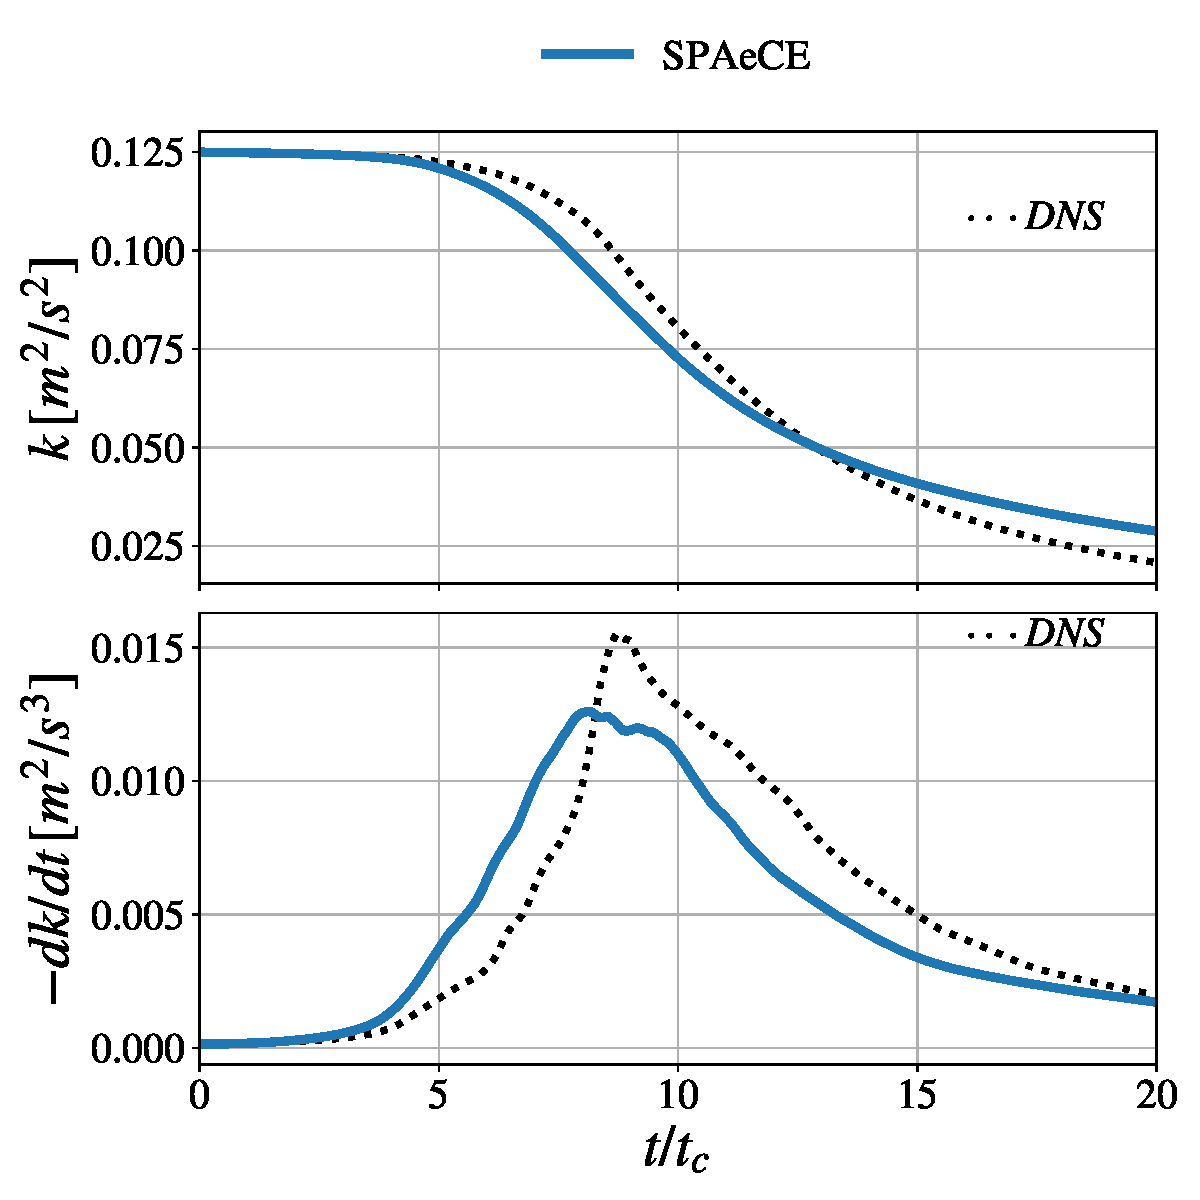
\includegraphics[width=\imgHalfWidth\columnwidth]{TGV3D/Re5000/spaece/65x65x65/3DTGV_Re5000_spaeceFoamCNTGV_dynKEqnHeinz_8x8_k_dkdt.pdf}\label{fig:TGV3D-5k65-KE}}
\subfloat[KE decay rate vs dissipation rate(s)]{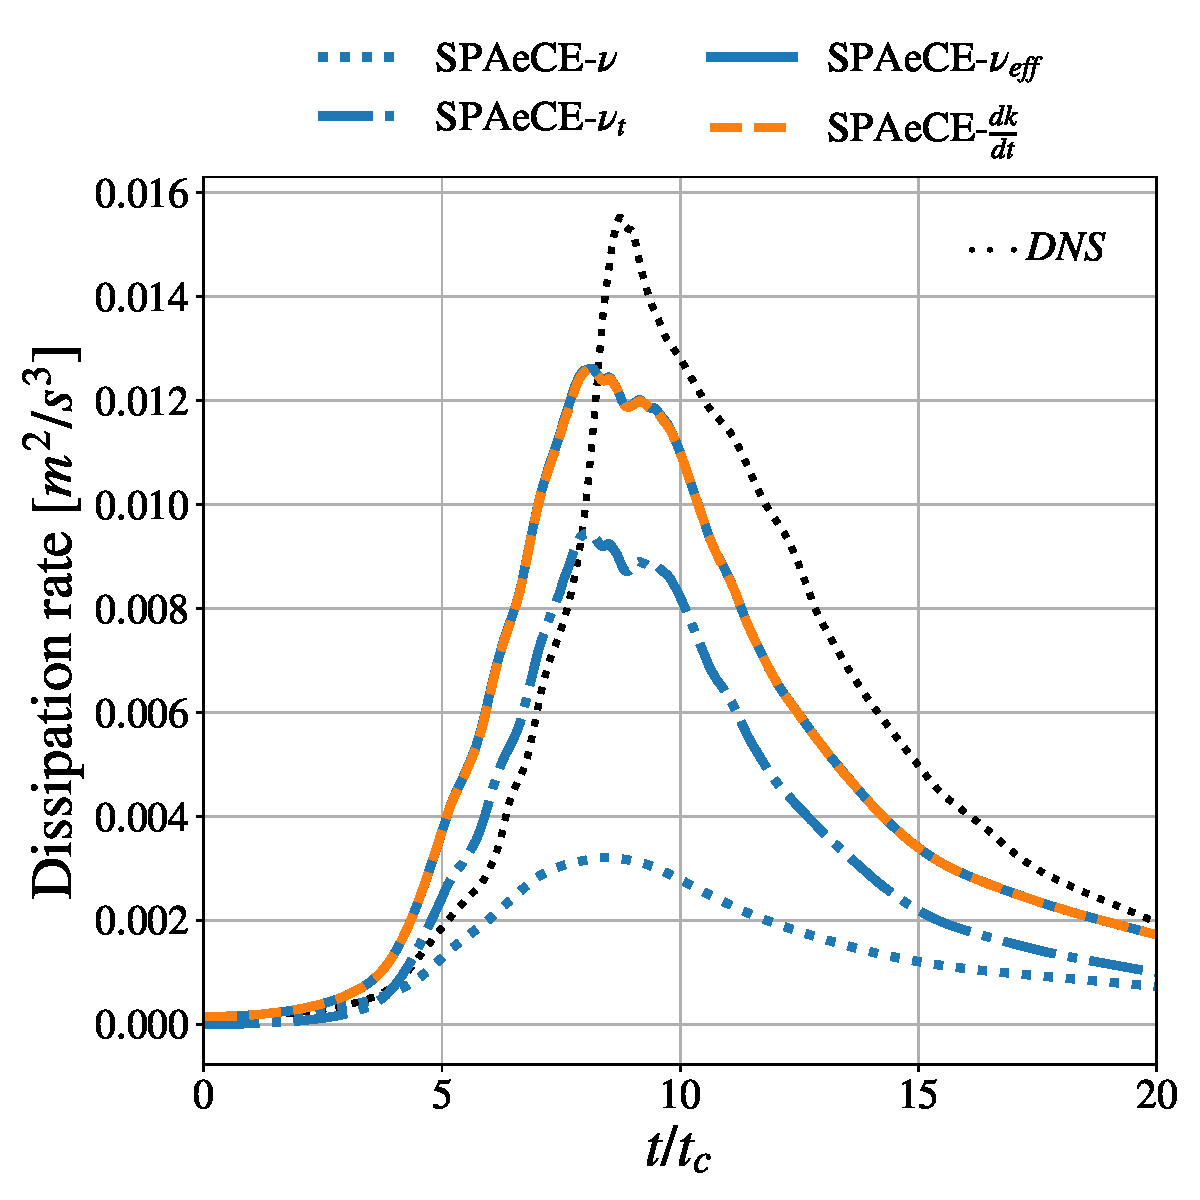
\includegraphics[width=\imgHalfWidth\columnwidth]{TGV3D/Re5000/spaece/65x65x65/3DTGV_Re5000_spaeceFoamCNTGV_dynKEqnHeinz_8x8_epsilon0.pdf}\label{fig:TGV3D-5k65-epsilon}} 
\caption{\spaeceA LES results of the 3D Taylor-Green vortex of $Re= 5 \times 10^3$ case with dynamic k equation turbulence model performed in a Cartesian cubic $65 \times 65 \times 65$ mesh} 
\label{fig:TGV3D-5k65}
\end{figure}

In Fig. \ref{fig:TGV3D-5k-3solver65}, KE decay rate and total dissipation rate from the \spaeceA, \spaeceARC and \piso algorithms are compared. Application of Rhie-Chow correction resulted in early dissipation in \spaeceARC and \piso algorithms compared to the \spaeceA algorithm (see Fig. \ref{fig:TGV3D-5k-3solver65-dkdt} at $t/t_c = 5$). Although, the differences in KE decay rate are small, the \piso algorithm has least total-dissipation rate ( i.e. most artificial dissipation) among the three algorithms. 

\begin{figure}[!h]
\centering
\subfloat[KE decay rate $ -\frac{dk}{dt}$]{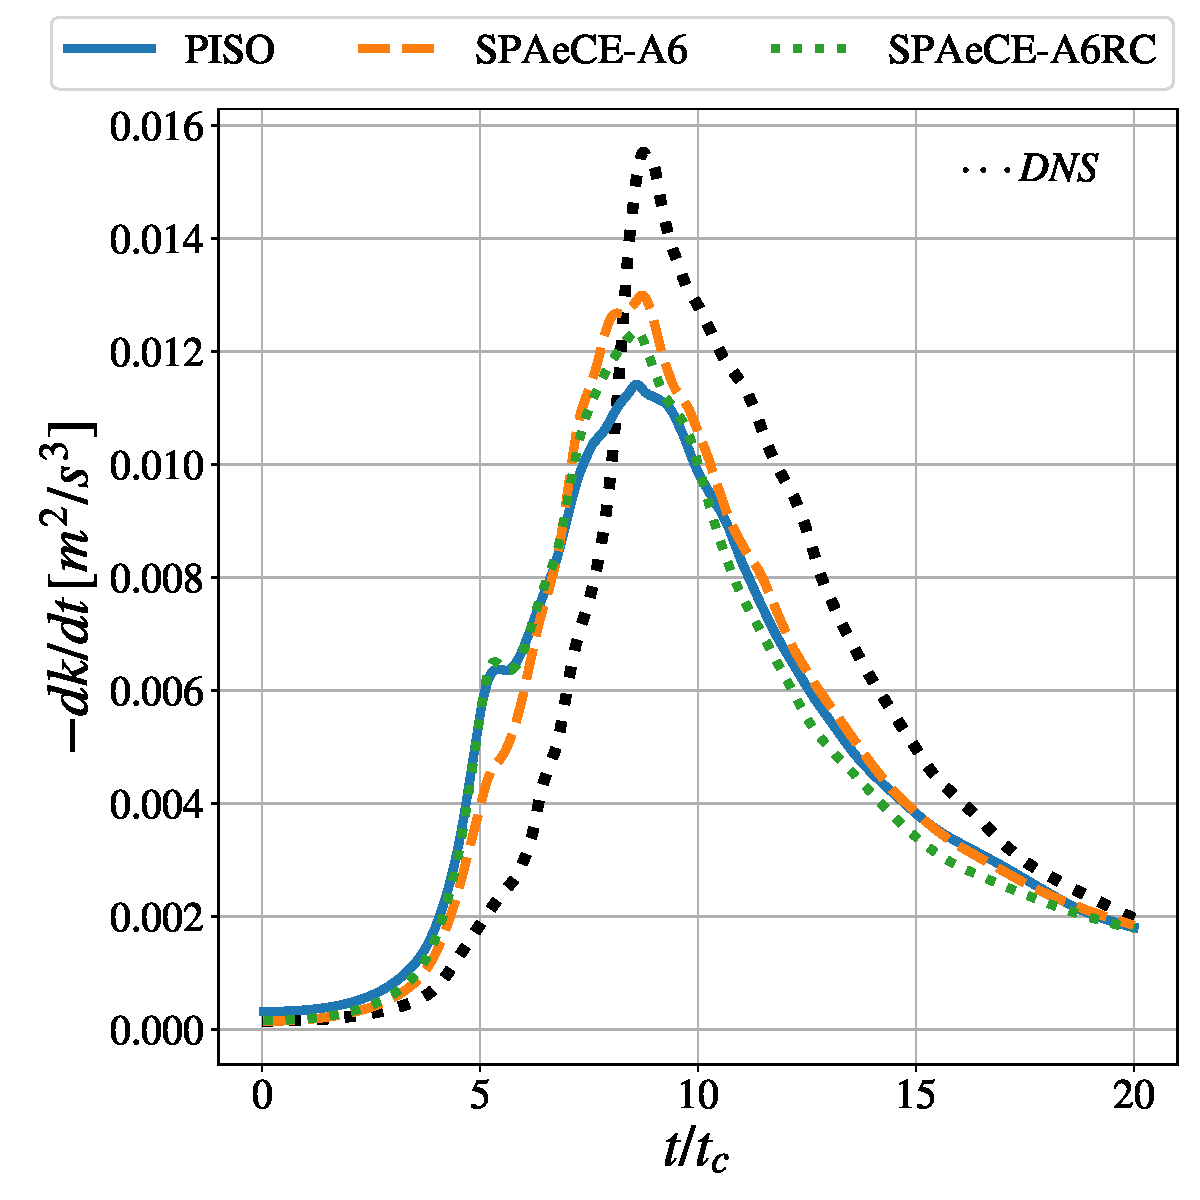
\includegraphics[width=\imgHalfWidth\columnwidth]{TGV3D/Re5000/pisoVsSpaeceA6VsA6RC/cube/65x65x65/3DTGV_Re5000_dynKEqnHeinz_8x8_dkdt.pdf}\label{fig:TGV3D-5k-3solver65-dkdt}}
\subfloat[Total dissipation rate $\nu_{eff}$]{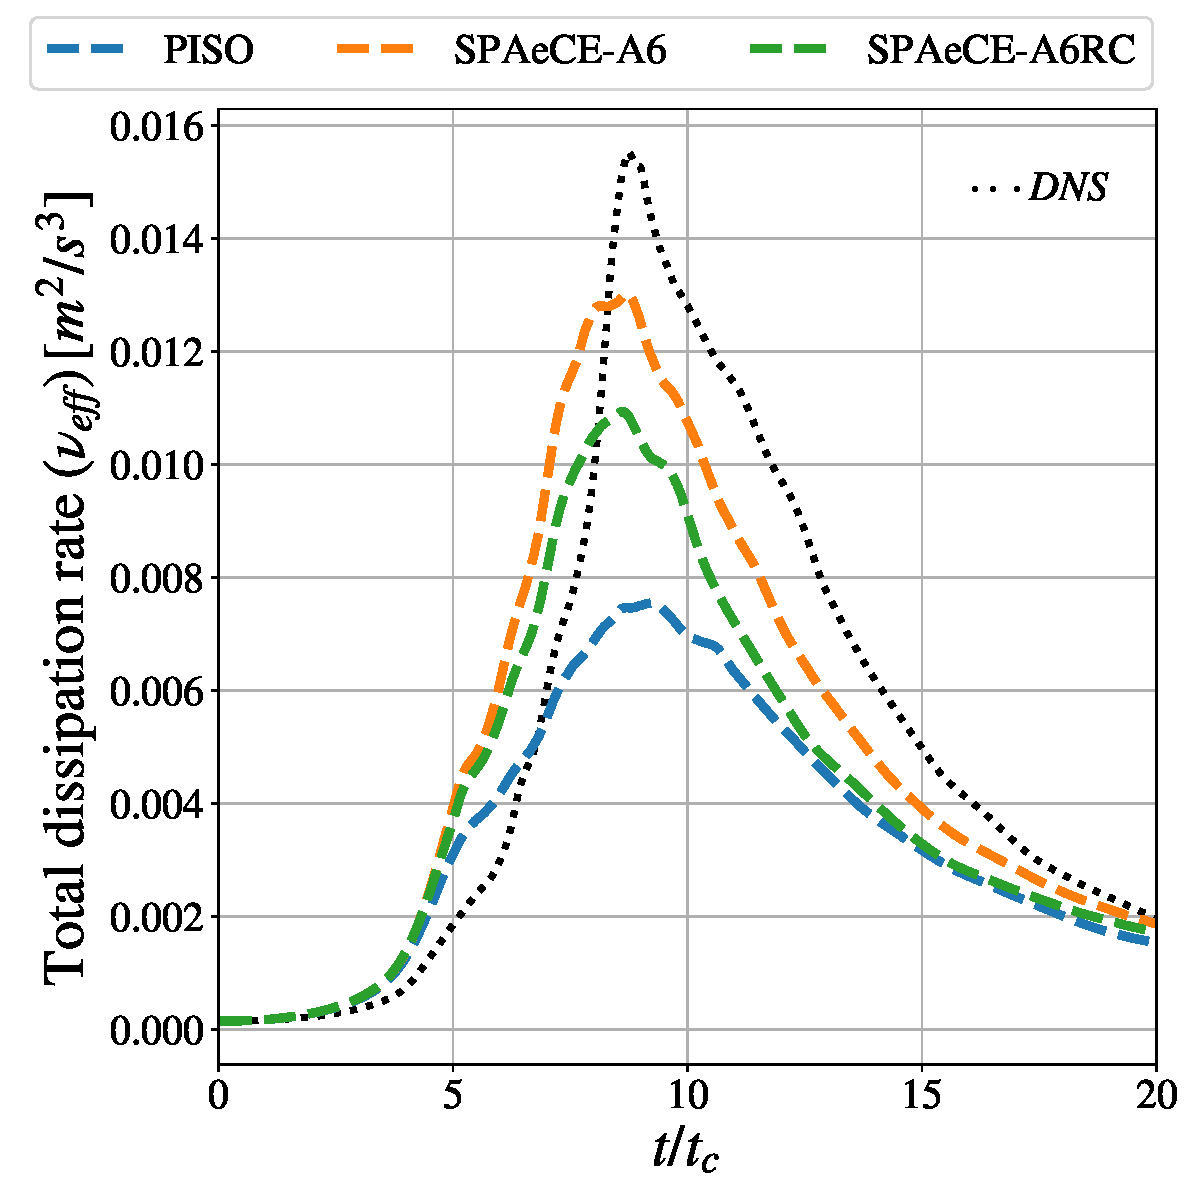
\includegraphics[width=\imgHalfWidth\columnwidth]{TGV3D/Re5000/pisoVsSpaeceA6VsA6RC/cube/65x65x65/3DTGV_Re5000_dynKEqnHeinz_8x8_nuEff.pdf}\label{fig:TGV3D-5k-3solver65-nuEff}} 
\caption{KE decay rate (left) and total dissipation rate (right) comparison for the 3D Taylor-Green vortex of $Re = 5\times10^3$ case among the \piso, \spaeceA and \spaeceARC algorithms performed in a Cartesian cubic $65 \times 65\times 65$ mesh} 
\label{fig:TGV3D-5k-3solver65}
\end{figure}


\begin{figure}[!h]
\centering
\subfloat[\spaeceARC algorithm]{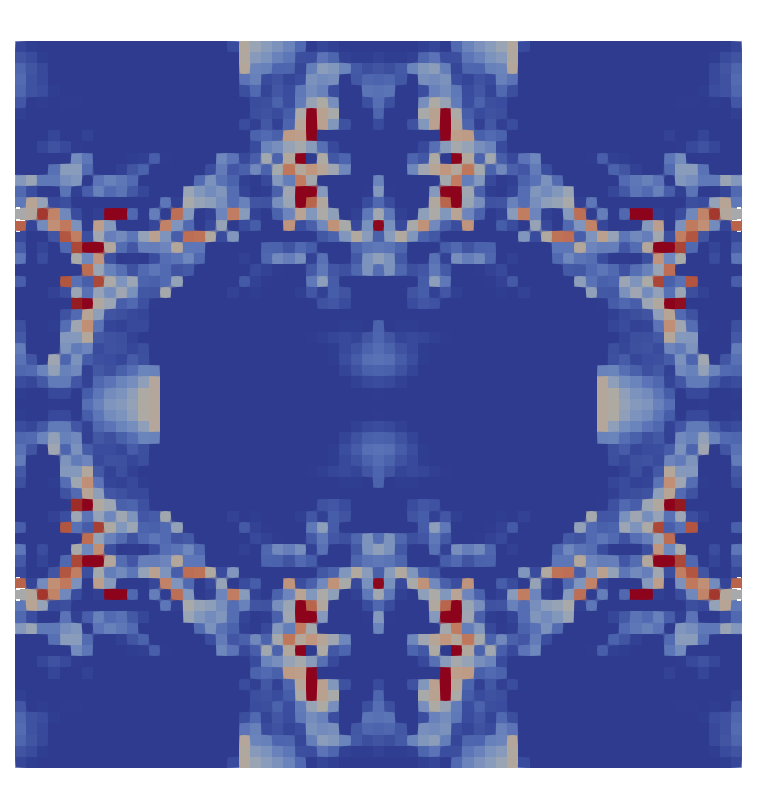
\includegraphics[width=\imgFortySeven\columnwidth]{TGV3D/Re5000/spaeceFoamCNTGV/A6RC/65cubed/spaeceA6RC_nut_time90.png}\label{fig:TGV3D-5kNut65-spaeceA6RC}}
\subfloat[\piso algorithm]{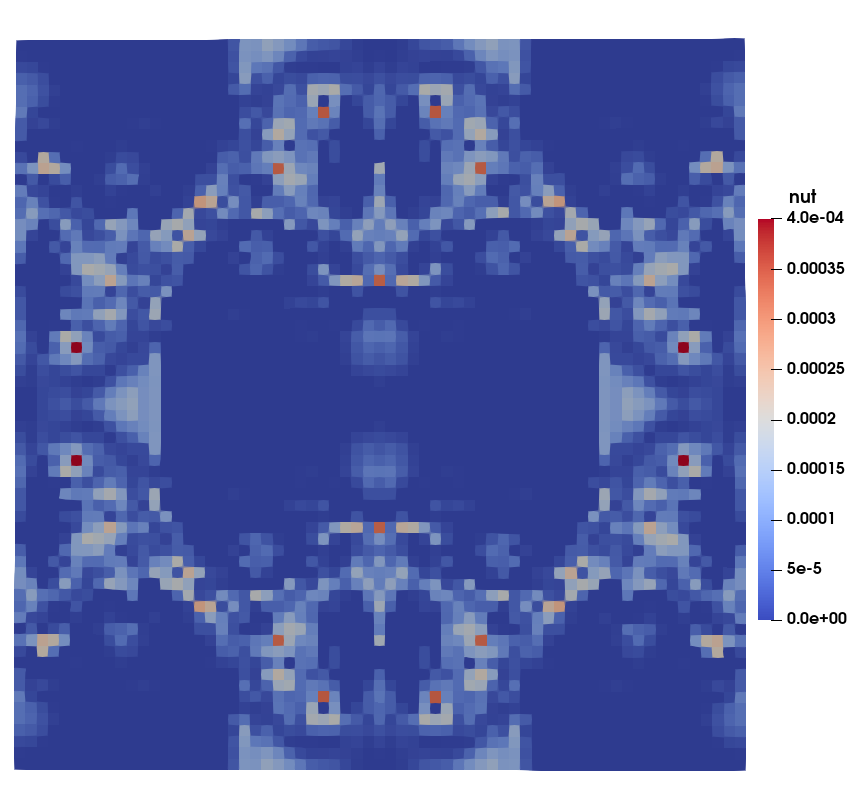
\includegraphics[width=\imgFiftyThree\columnwidth]{TGV3D/Re5000/pisoFoamMod/65cubed/piso_nut_time90.png}\label{fig:TGV3D-5kNut65-piso}} 
\caption{Eddy viscosity $\nu_t$ comparison for the 3D Taylor-Green vortex of $Re = 5\times10^3$ case between the \spaeceARC and \piso algorithms performed in a Cartesian cubic $65 \times 65\times 65$ mesh} 
\label{fig:TGV3D-5kNut65}
\end{figure}


When compared to the artificial dissipation free \spaeceA algorithm, the Rhie-Chow corrected \spaeceARC algorithm has moderate artificial dissipation present. However, it shows a significant improvement over the \piso algorithm. Fig. \ref{fig:TGV3D-5kNut65} compares the eddy viscosity $\nu_t$ in the $y =0$ cross-section at time $t/t_c = 9$, where the \spaeceARC algorithm shows substantially higher eddy viscosity $\nu_t$ values compared to the \piso algorithm.

%\clearpage
%\newpage

%\line(x-slope,y-slope){length}
%\line(1,0){300}

%\rule{length}{thickness}
%\rule{\paperwidth}{1pt}
%\rule{\textwidth}{1pt}

\subsubsection[Cartesian cubic 129x129x129 mesh:]{Influence of mesh refinement: Cartesian cubic $129 \times 129 \times 129$ mesh} 
\label{sec:TGV3D-Cart129}
Following the previous section, the 3D Taylor-Green vortex is simulated in refined Cartesian cubic $129 \times 129 \times 129$ mesh. Compared to the coarse mesh, LES on the refined mesh resolves more scales, thus have less SFS stress (Fig \ref{fig:TGV3D-5k129-epsilon}). The effect early aggressive dissipation by the dynamic SFS model is reduced albeit present! This signifies importance of accurate SFS scale model in DNS. Similar to the coarse mesh, the \spaeceARC algorithm has substantially less artificially dissipation (Fig \ref{fig:TGV3D-5k-3solver-129}) and higher eddy viscosity $\nu_t$ values (Fig. \ref{TGV3D-5kNut129}) compared to the \piso algorithm. 

\begin{figure}[!h]
\centering
\subfloat[KE decay (top) and decay rate (bottom)]{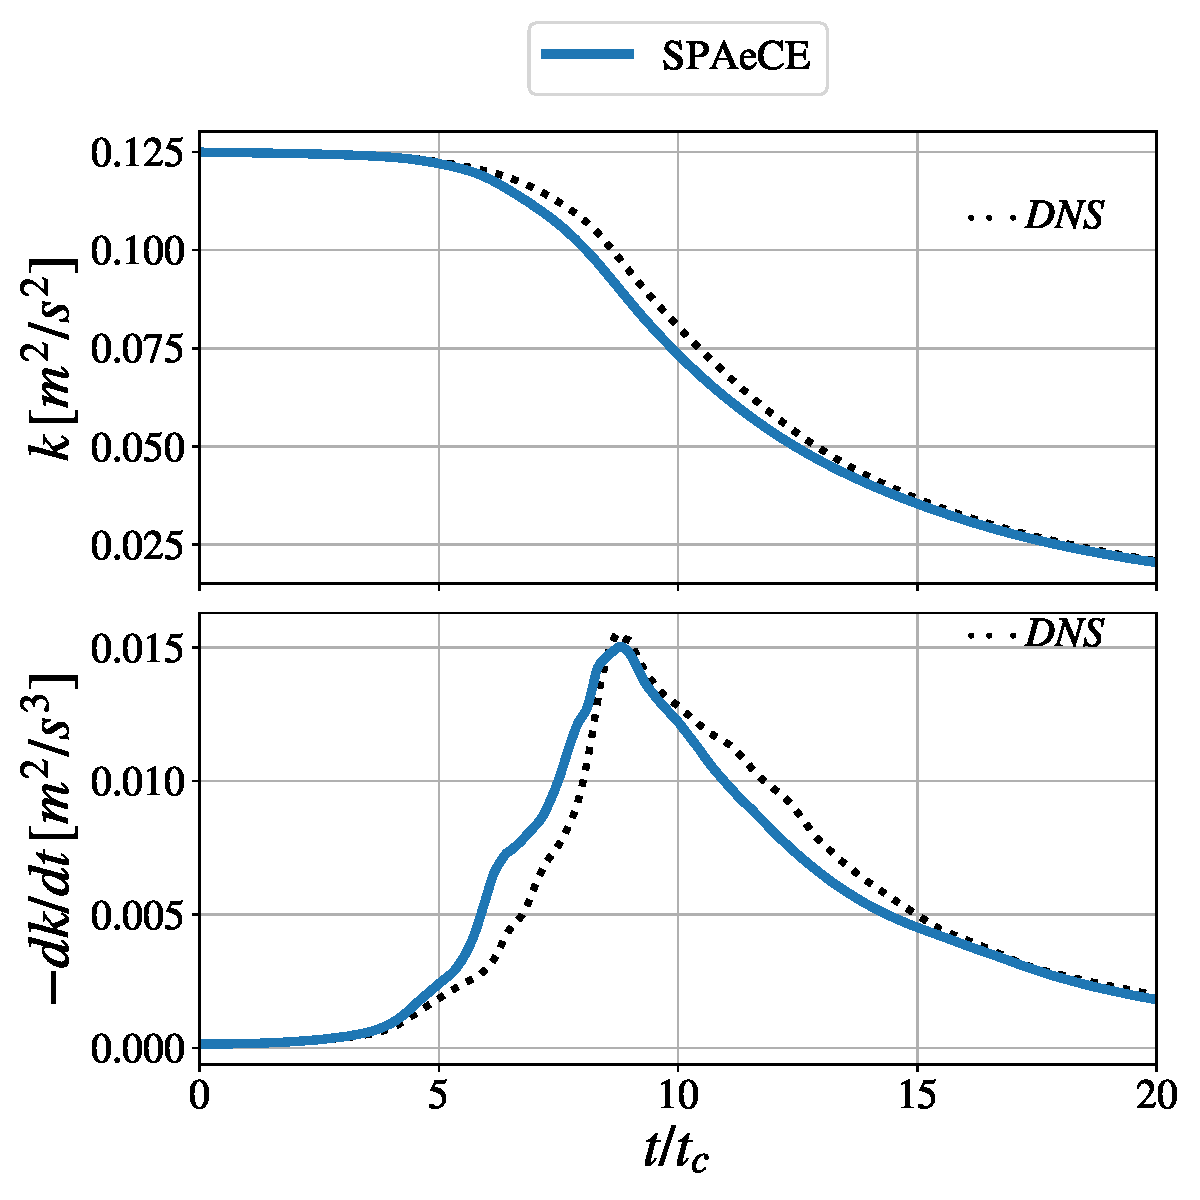
\includegraphics[width=\imgHalfWidth\columnwidth]{TGV3D/Re5000/spaece/129x129x129/3DTGV_Re5000_spaeceFoamCNTGV_dynKEqnHeinz_8x8_k_dkdt.pdf}\label{fig:TGV3D-5k129-KE}}
\subfloat[KE decay rate vs dissipation rate(s)]{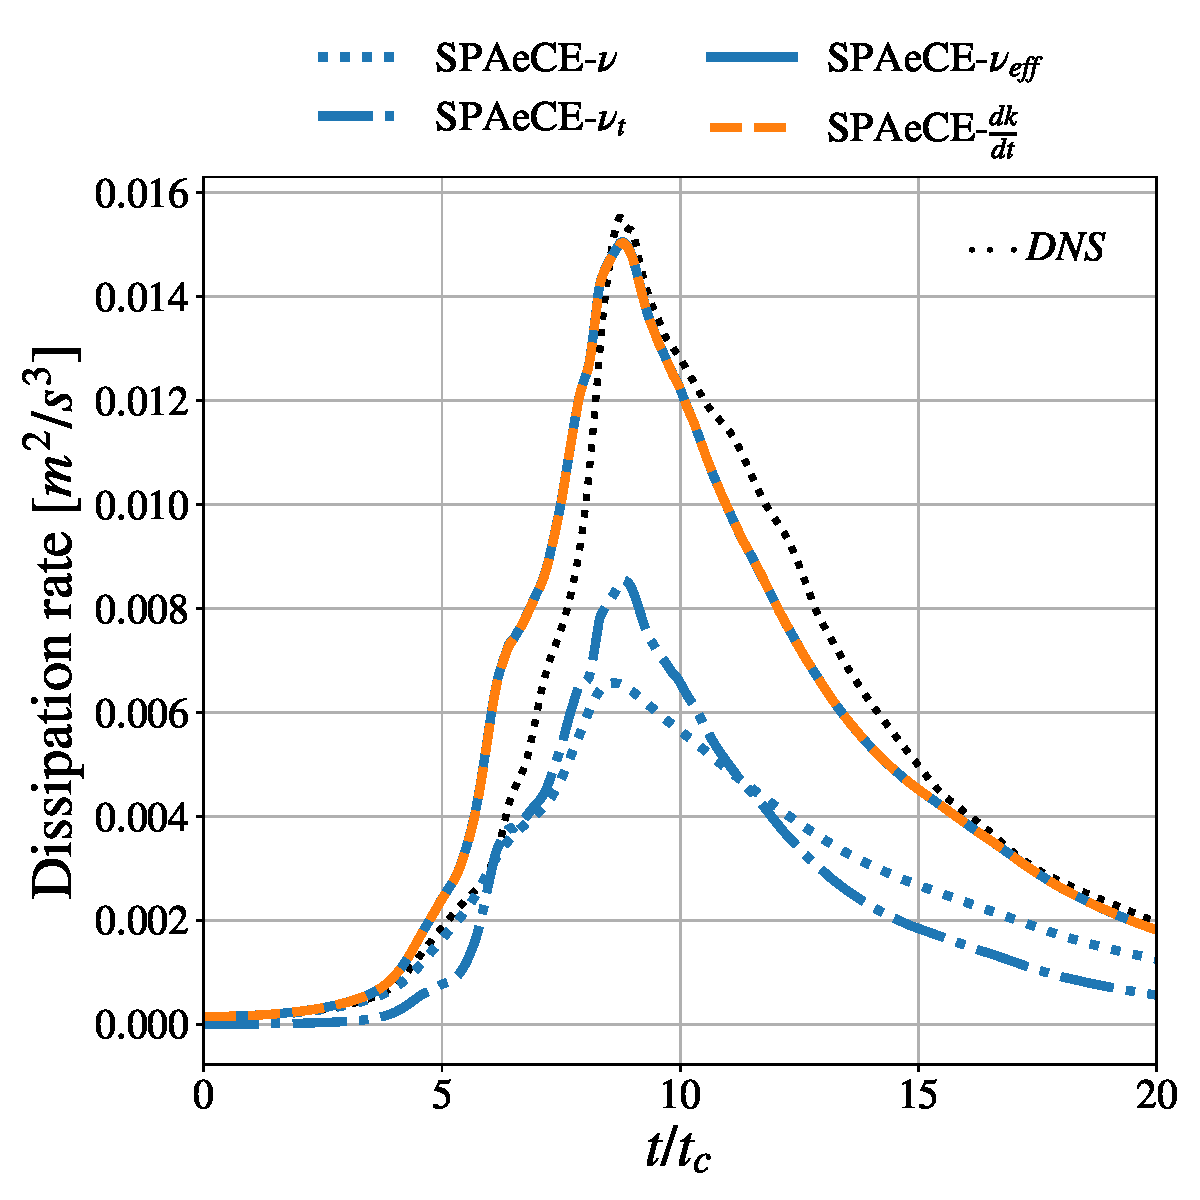
\includegraphics[width=\imgHalfWidth\columnwidth]{TGV3D/Re5000/spaece/129x129x129/3DTGV_Re5000_spaeceFoamCNTGV_dynKEqnHeinz_8x8_epsilon0.pdf}\label{fig:TGV3D-5k129-epsilon}} 
\caption{\spaeceA LES results of the 3D Taylor-Green vortex of $Re= 5 \times 10^3$ case with dynamic k equation turbulence model performed in a Cartesian cubic $129 \times 129 \times 129$ mesh} 
\label{fig:TGV3D-5k129}
\end{figure}



\begin{figure}[!h]
\centering
\subfloat[KE decay rate $ -\frac{dk}{dt}$]{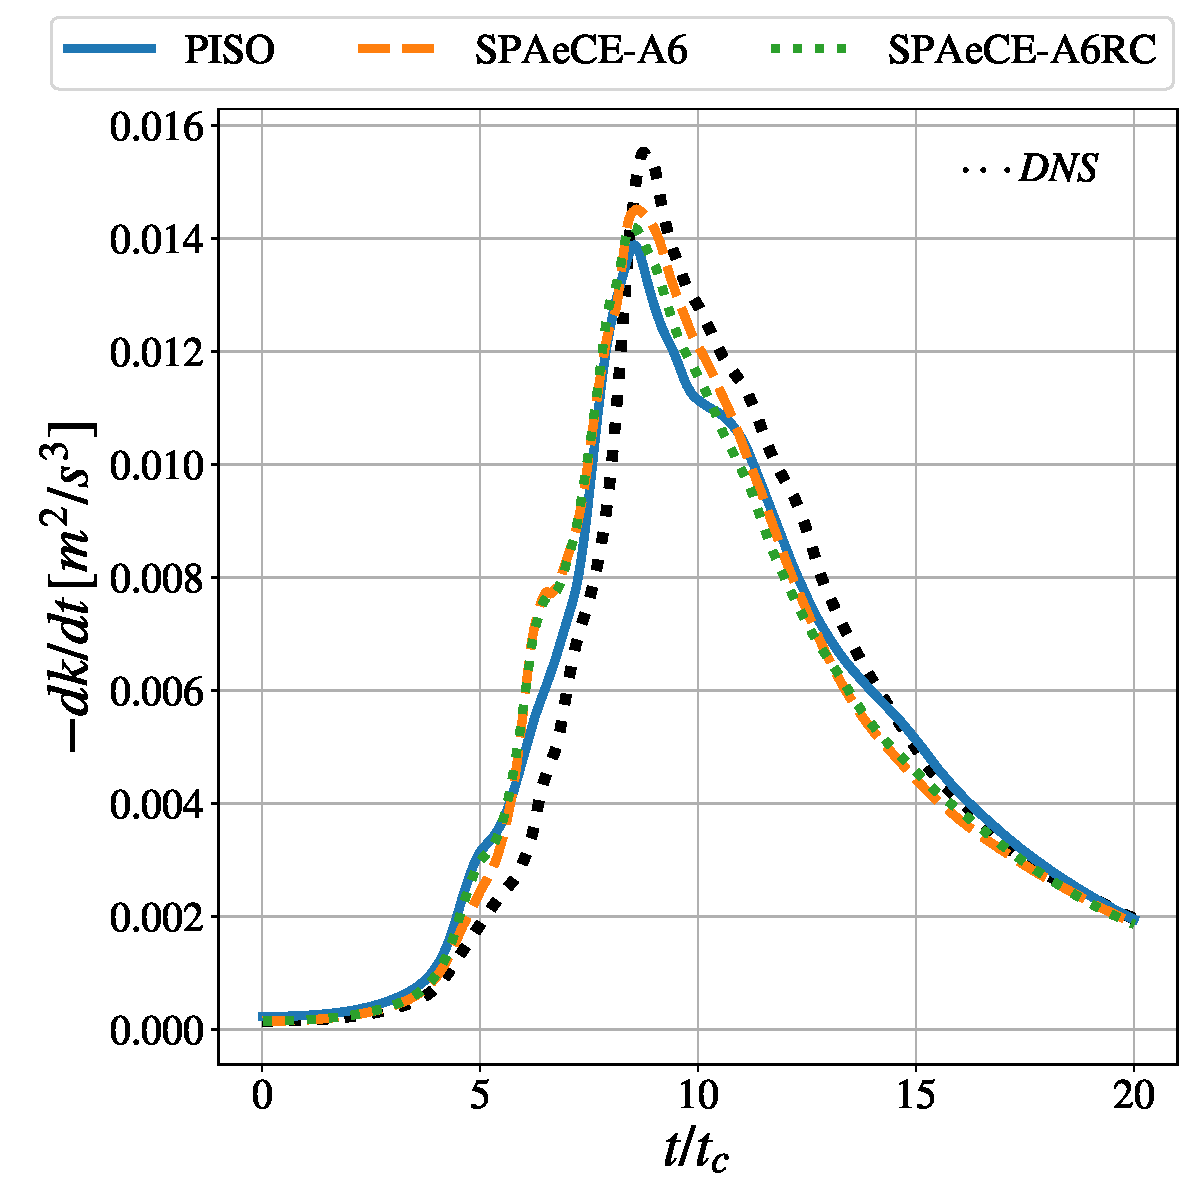
\includegraphics[width=\imgHalfWidth\columnwidth]{TGV3D/Re5000/pisoVsSpaeceA6VsA6RC/cube/129x129x129/3DTGV_Re5000_dynKEqnHeinz_8x8_dkdt.pdf}\label{fig:TGV3D-5k-3solver-129-dkdt}}
\subfloat[Total dissipation rate $\nu_{eff}$]{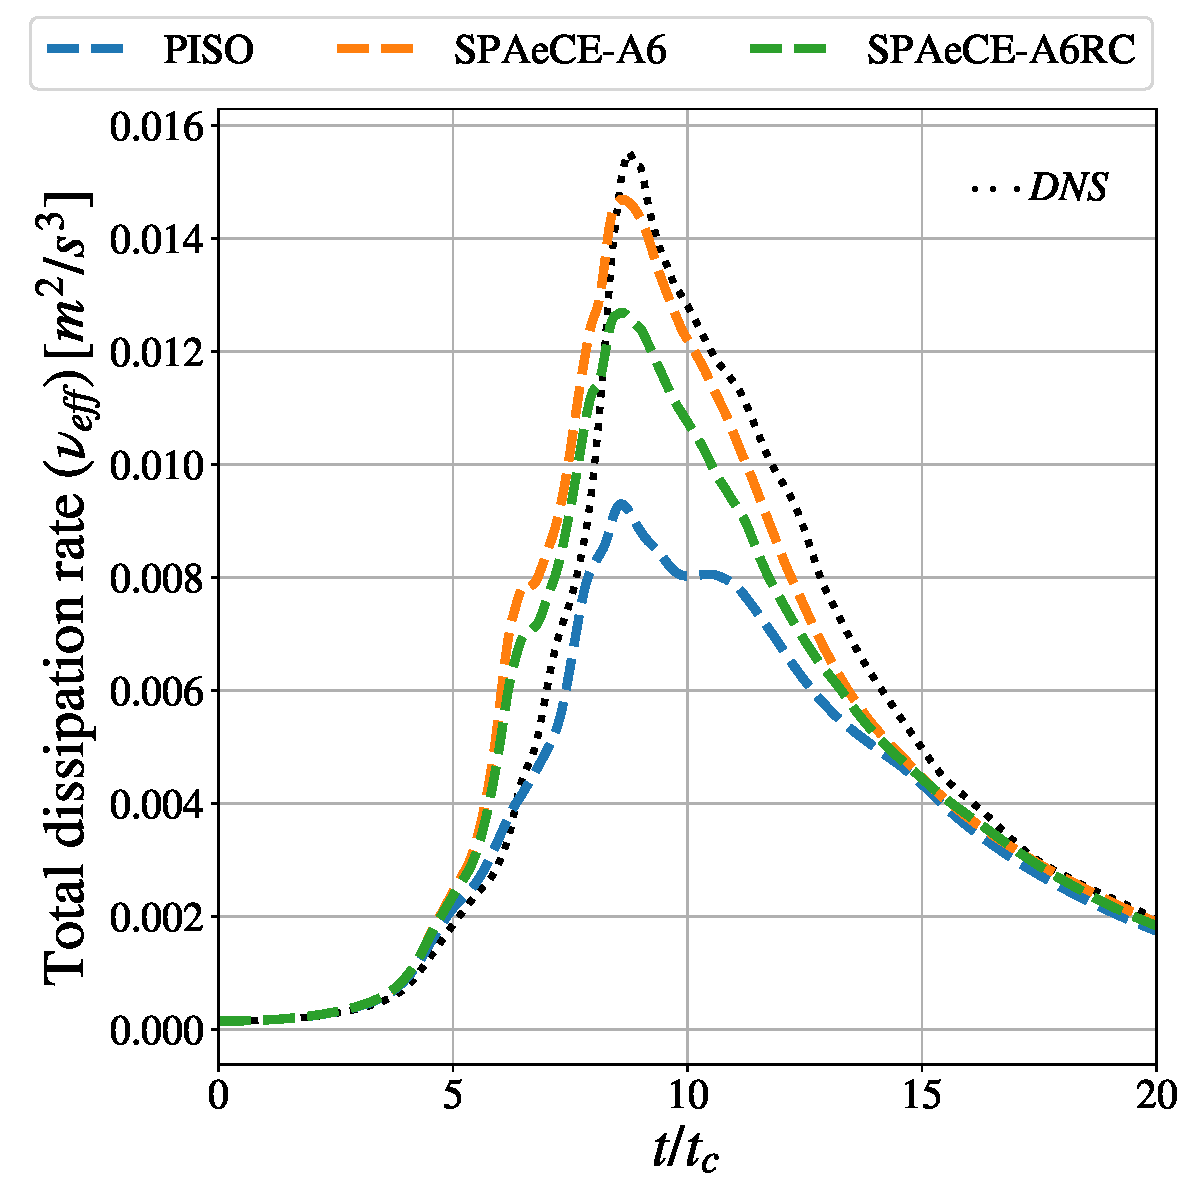
\includegraphics[width=\imgHalfWidth\columnwidth]{TGV3D/Re5000/pisoVsSpaeceA6VsA6RC/cube/129x129x129/3DTGV_Re5000_dynKEqnHeinz_8x8_nuEff.pdf}\label{fig:TGV3D-5k-3solver-129-nuEff}} 
\caption{KE decay rate (left) and total dissipation rate (right) comparison among the \piso, \spaeceA and \spaeceARC algorithms performed in a Cartesian cubic $129 \times 129 \times 129$ mesh} 
\label{fig:TGV3D-5k-3solver-129}
\end{figure}


\begin{figure}[!h]
\centering
\subfloat[\spaeceARC algorithm]{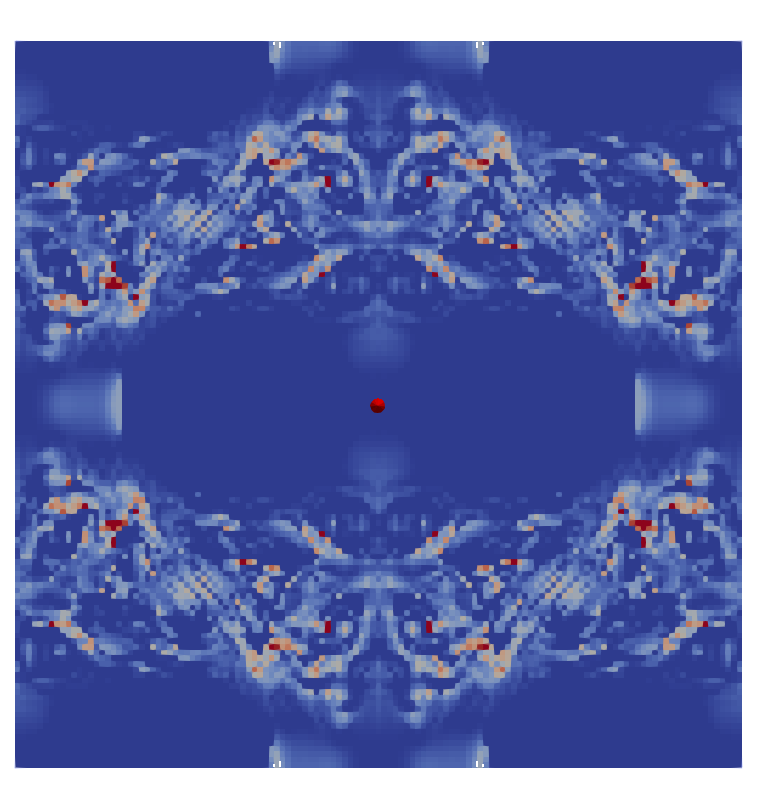
\includegraphics[width=\imgFortySeven\columnwidth]{TGV3D/Re5000/spaeceFoamCNTGV/A6RC/129cubed/spaeceA6RC_nut_time90}\label{fig:TGV3D-5kNut129-spaeceA6RC}}
\subfloat[\piso algorithm]{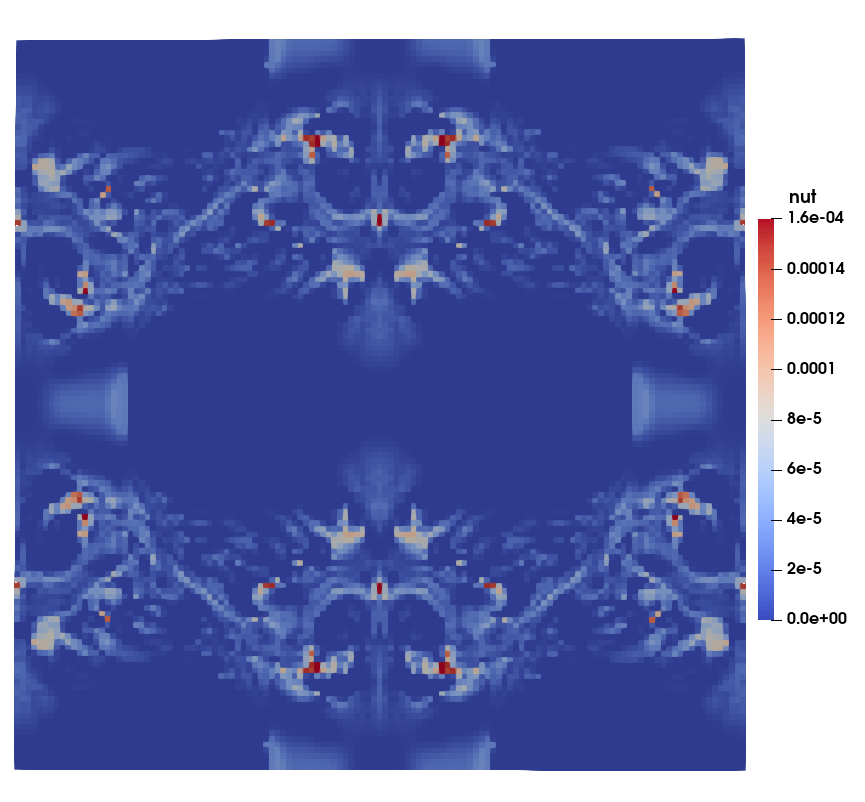
\includegraphics[width=\imgFiftyThree\columnwidth]{TGV3D/Re5000/pisoFoamMod/129cubed/piso_nut_time90}\label{fig:TGV3D-5kNut129-piso}} 
\caption{Eddy viscosity $\nu_t$ comparison for the 3D Taylor-Green vortex of $Re = 5\times10^3$ case between the \spaeceARC and \piso algorithms performed in a Cartesian cubic $129 \times 129 \times 129$ mesh} 
\label{fig:TGV3D-5kNut129}
\end{figure}





\clearpage
\subsubsection[Right-angle triangulated prismatic (65x65)x2x65 mesh]{Influence of non-orthogonality: Right-angle triangulated prismatic $(65 \times 65) \times 2 \times 65$ mesh}
\label{sec:TGV3D-prism}
Each control volume of the Cartesian cubic $65 \times 65 \times 65$ mesh is split diagonally in $z$ normal plane to convert the cube into two right-angle prism, resulting in a $(65 \times 65) \times 2 \times 65$ mesh. The prism has three orthogonal and two non-orthogonal faces. Similar to the Cartesian cubic meshes (Sec. \ref{sec:TGV3D-Cart65} and \ref{sec:TGV3D-Cart129}), the \spaeceA algorithm doesn't introduce and non-physical dissipation (Fig. \ref{fig:TGV3D-5kPrism-3solver65-dkdt}) and the \spaeceARC algorithm has higher total-dissipation rate compared to the \piso algorithm (Fig. \ref{fig:TGV3D-5kPrism-3solver65-nuEff}).     

\begin{figure}[!h]
\centering
\subfloat[KE decay rate $ -\frac{dk}{dt}$]{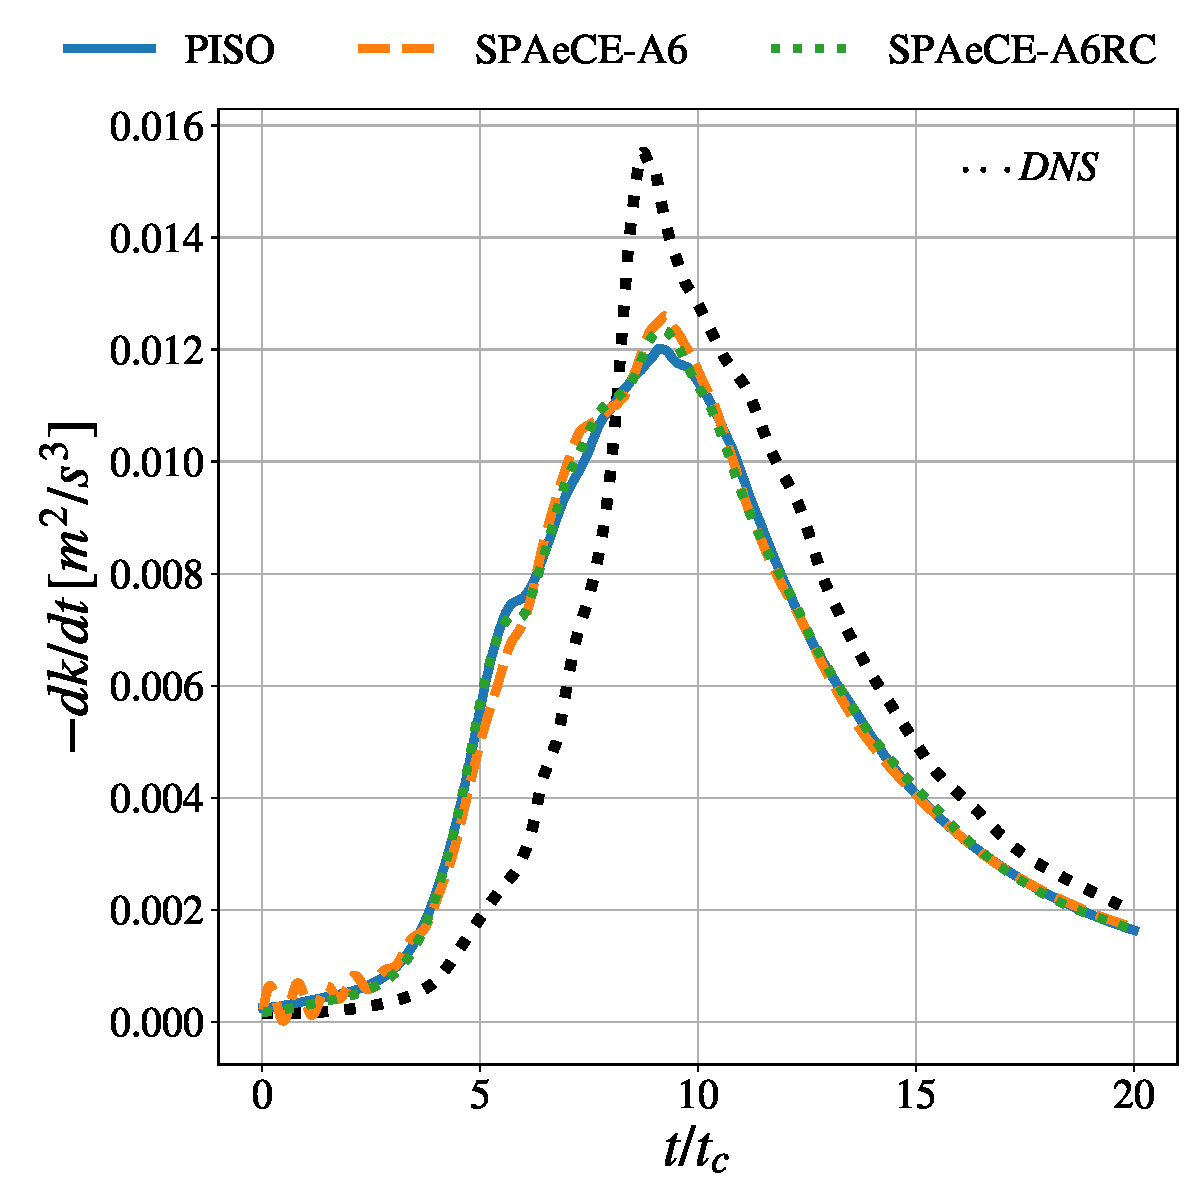
\includegraphics[width=\imgHalfWidth\columnwidth]{TGV3D/Re5000/pisoVsSpaeceA6VsA6RC/prism/65x65x65/3DTGV_unstructured_uniformRightAnglePrism_Re5000_dynKEqnHeinz_8x8_dkdt.pdf}\label{fig:TGV3D-5kPrism-3solver65-dkdt}}
\subfloat[Total dissipation rate $\nu_{eff}$]{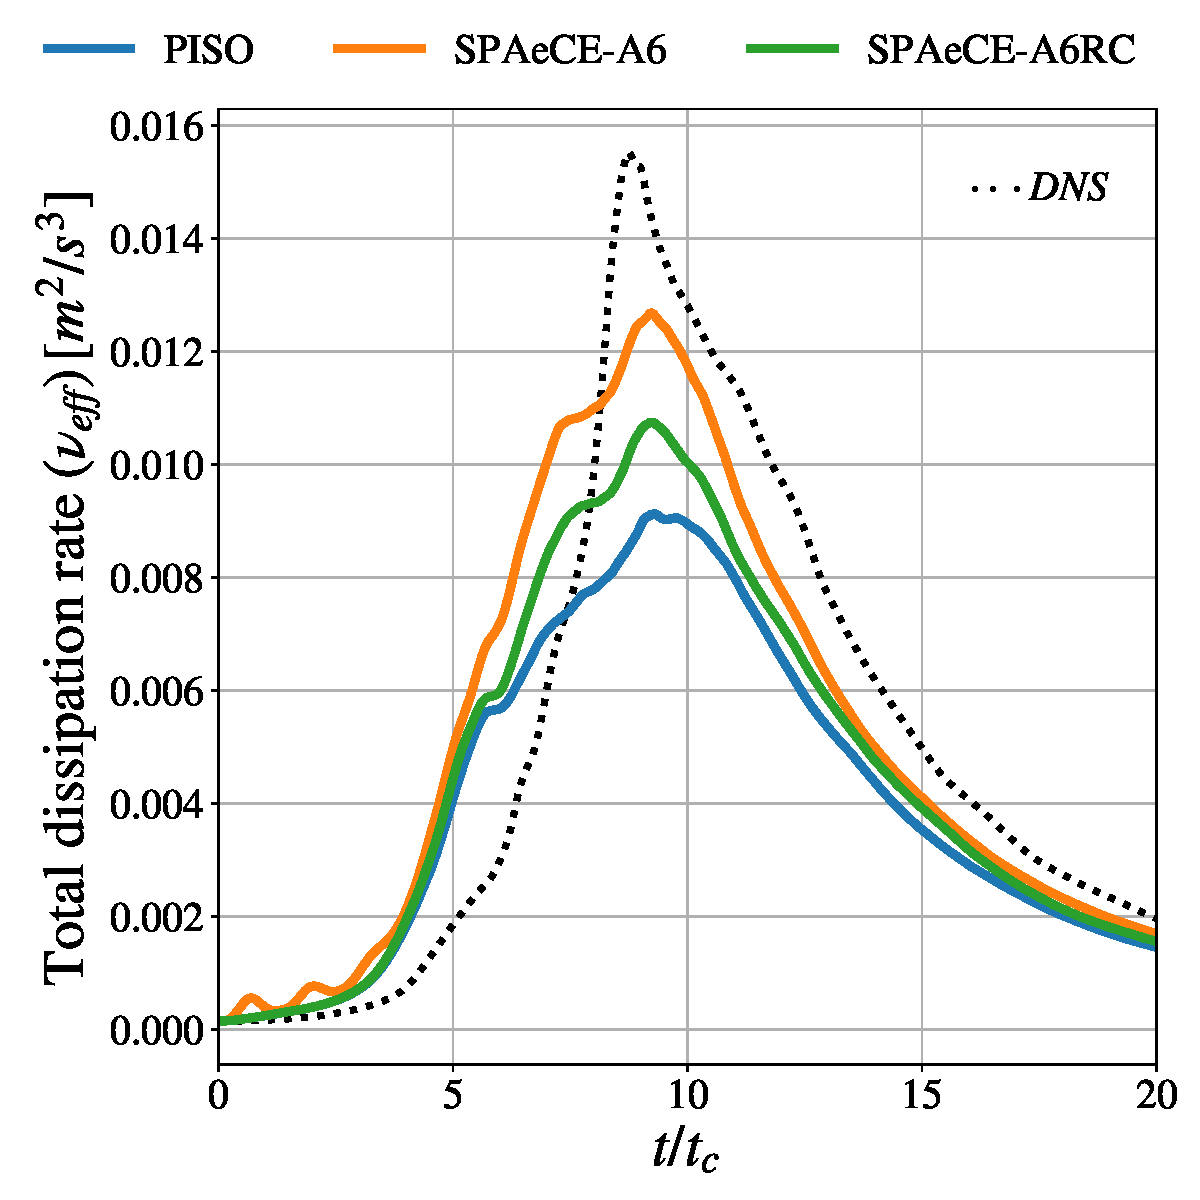
\includegraphics[width=\imgHalfWidth\columnwidth]{TGV3D/Re5000/pisoVsSpaeceA6VsA6RC/prism/65x65x65/3DTGV_unstructured_uniformRightAnglePrism_Re5000_dynKEqnHeinz_8x8_nuEff.pdf}\label{fig:TGV3D-5kPrism-3solver65-nuEff}} 
\caption{KE decay rate (left) and total dissipation rate (right) comparison for the 3D Taylor-Green vortex of $Re = 5\times10^3$ case among the \piso, \spaeceA and \spaeceARC algorithms performed in a right-angle triangulated prismatic $(65 \times 65) \times 2 \times 65$ mesh} 
\label{fig:TGV3D-5kPrism-3solver65}
\end{figure}

\subsubsection{Influence of non-uniform mesh}
\label{sec:TGV3D-nonUniform}

In Fig. \ref{fig:TGV3D-inv-hex}, we have shown the importance of using the mid-point interpolation scheme instead of a linear scheme for KE conservation in a non-uniform Cartesian hexagonal $65 \times 65 \times 65$ mesh. However, the mid-point interpolation in a non-uniform mesh provides less than 2nd order accuracy thus influence the overall results. Fig. \ref{fig:3DTGV-5k-CubeHex} compares the 3D Taylor-Green vortex of $Re = 5\times10^3$ results between the cubic and hexagonal mesh. Although both meshes are Cartesian and have the same cell count, the non-uniform hexagonal mesh is slightly more dissipative and less accurate compared to corresponding uniform, cubic mesh. Thus with mid-point interpolation, accuracy is traded off for KE conservation and stability.

\begin{figure}[!h]
\centering
\subfloat[KE decay (top) and decay rate (bottom)]{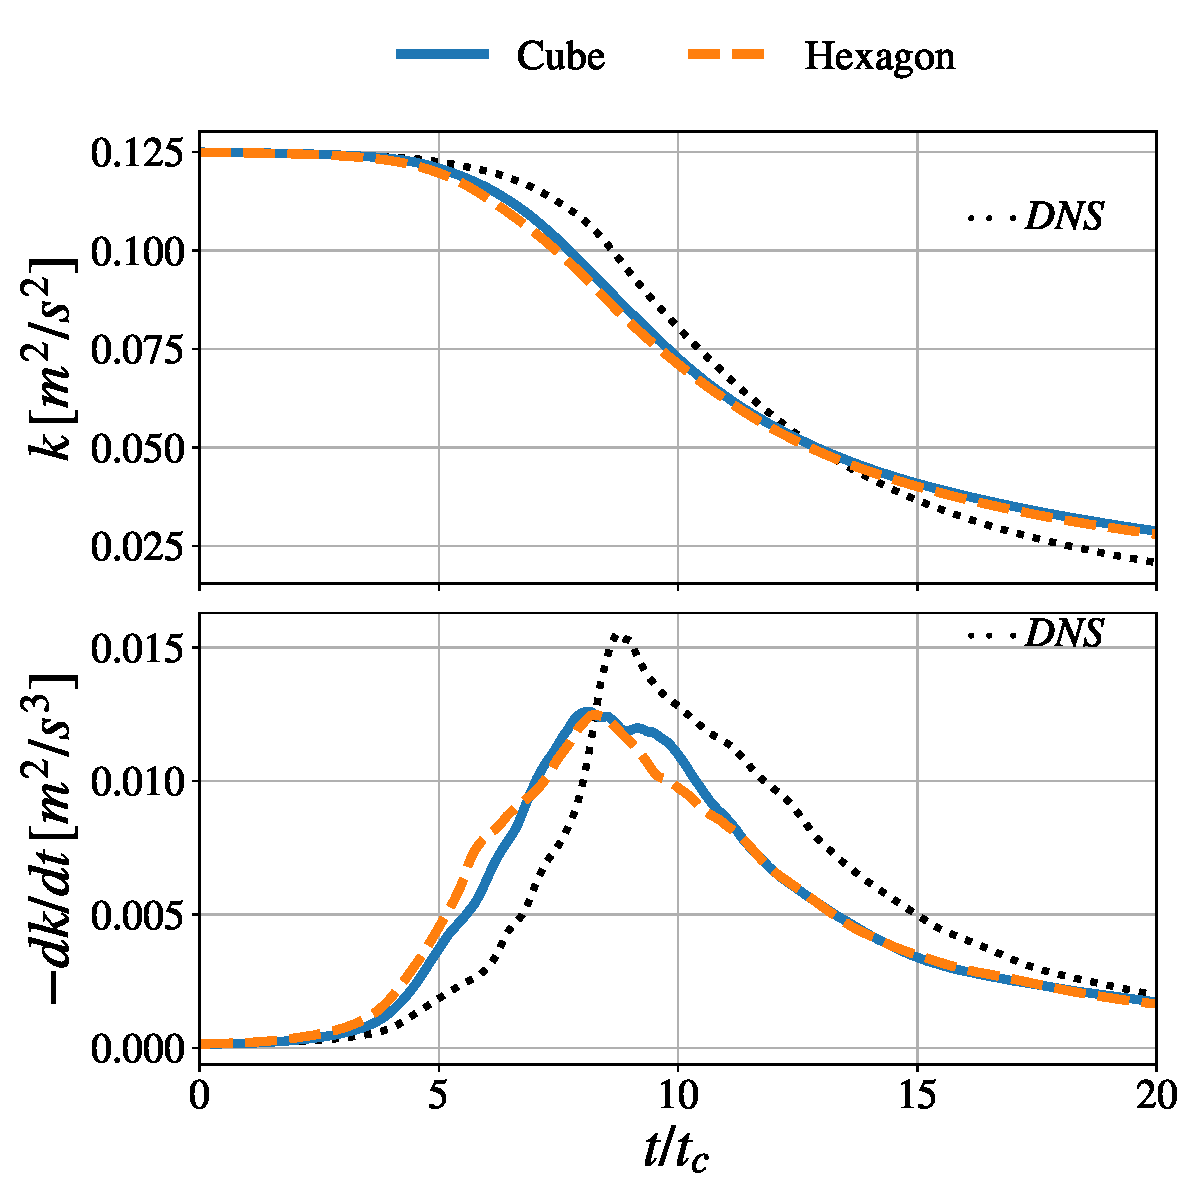
\includegraphics[width=\imgHalfWidth\columnwidth]{TGV3D/Re5000/cubeVsHex/65x65x65/3DTGV_Re5000_spaeceFoamCNTGV_dynKEqnHeinz_8x8_k_dkdt.pdf}\label{fig:label one}}
\subfloat[KE decay rate vs dissipation rate(s)]{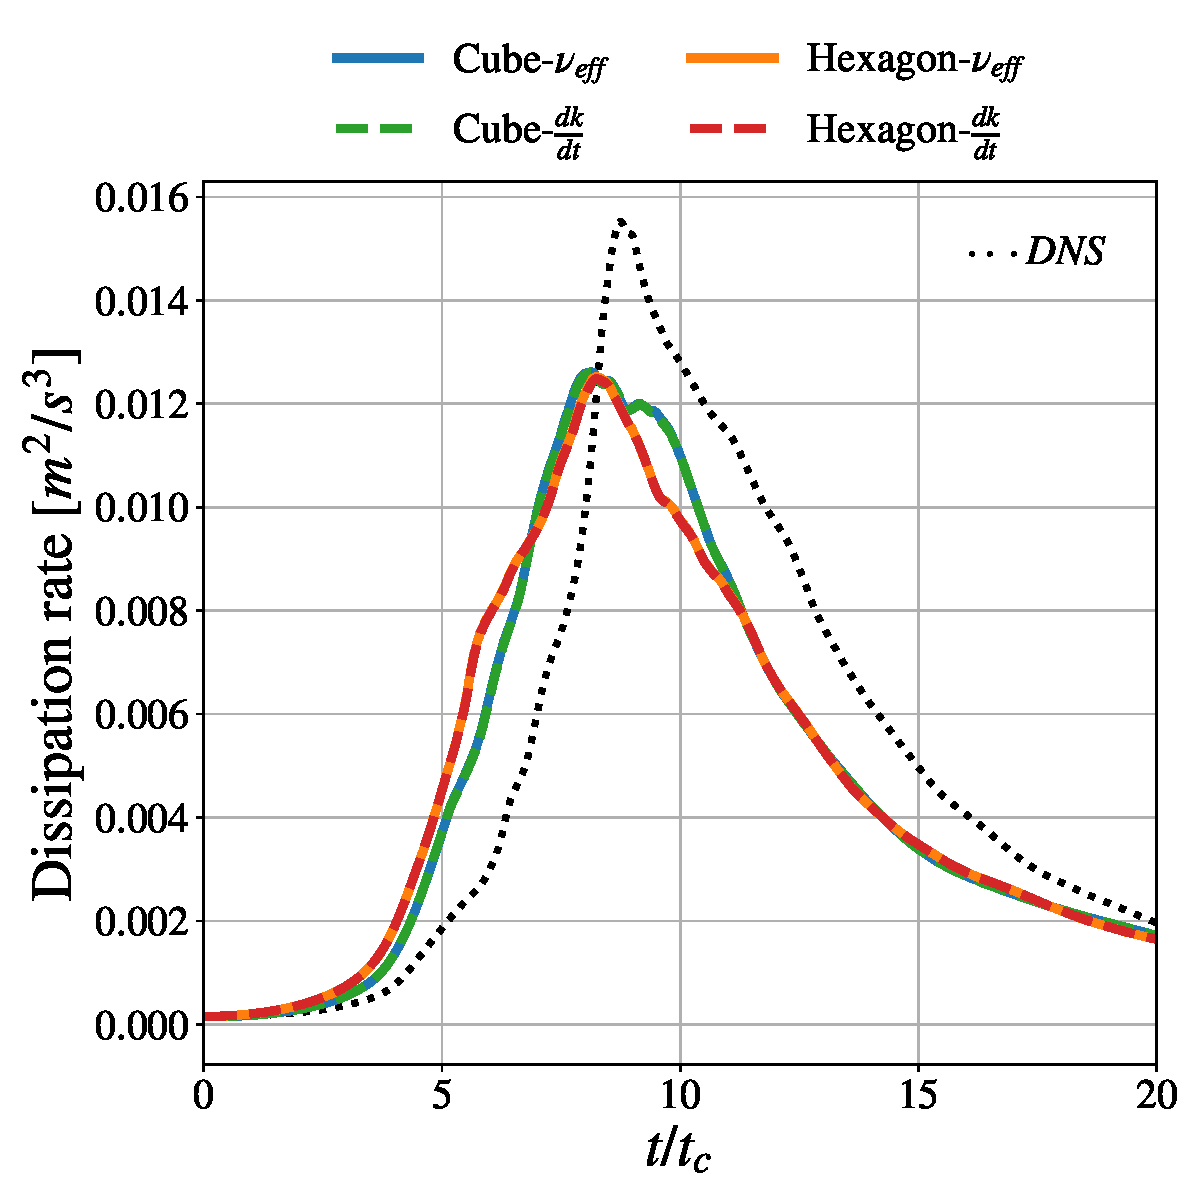
\includegraphics[width=\imgHalfWidth\columnwidth]{TGV3D/Re5000/cubeVsHex/65x65x65/3DTGV_Re5000_spaeceFoamCNTGV_dynKEqnHeinz_8x8_epsDkdt0.pdf}\label{fig:3DTGV-5k-CubeHex-dissp}} 
\caption{\spaeceA LES results of the 3D Taylor-Green vortex of $Re= 5 \times 10^3$ case with dynamic k equation turbulence model compared between a Cartesian uniform-cubic mesh and a Cartesian non-uniform hexagonal mesh (max. aspect ratio $5.3$) of $65 \times 65 \times 65$ cells} 
\label{fig:3DTGV-5k-CubeHex}
\end{figure}










\clearpage
\subsection[Fully developed channel flow at Re_tau 590]{Fully developed channel flow at $Re_\tau = 590$}
\label{sec:channel590}

Fully developed turbulent flow though a plane channel at Reynolds number based on friction velocity $Re_\tau = 590$ is investigated.
A 3D computational domain formed for channel dimension $(L \times W \times H): 2\pi \times \pi \times 2$. A Cartesian hexagonal $129 \times 129 \times 129$ mesh is used, which is symmetric at the channel boundary layer height $y=1$. The mesh resolution is uniform in the stream-wise and cross-stream direction, and in wall-normal direction, gradually stretched from next-to-wall resolution $y^+ \leqslant 0.5$ (cell center height of the wall adjacent control volumes). The normalized resolution in the stream-wise direction is $x^+ \leqslant 30$ and cross-stream direction is $z^+ \leqslant 15$. The maximum cell aspect ratio at near-wall cells is $\approx 32$ gradually decreased to $1$ at the boundary layer height.

Periodic boundary condition is applied in the stream-wise and cross-stream directions, and no-slip boundary velocity and zero-gradient pressure is applied at channel walls. A time-varying, uniform driving pressure gradient included as a source term in the momentum conservation equation to maintain mean flow rate across the channel constant. LES is performed for three different algorithms \piso, \spaece and \spaeceARC and the dynamic k equation model of Heinz et al. is utilized as the sub-filter-stress model. The regularization and LES filter are defined same as in the 3D ataylor-Green vortex case (Sec. \ref{sec:3DTGV}).

\begin{figure}[!h]
\centering
\subfloat[Mean streamwise velocity]{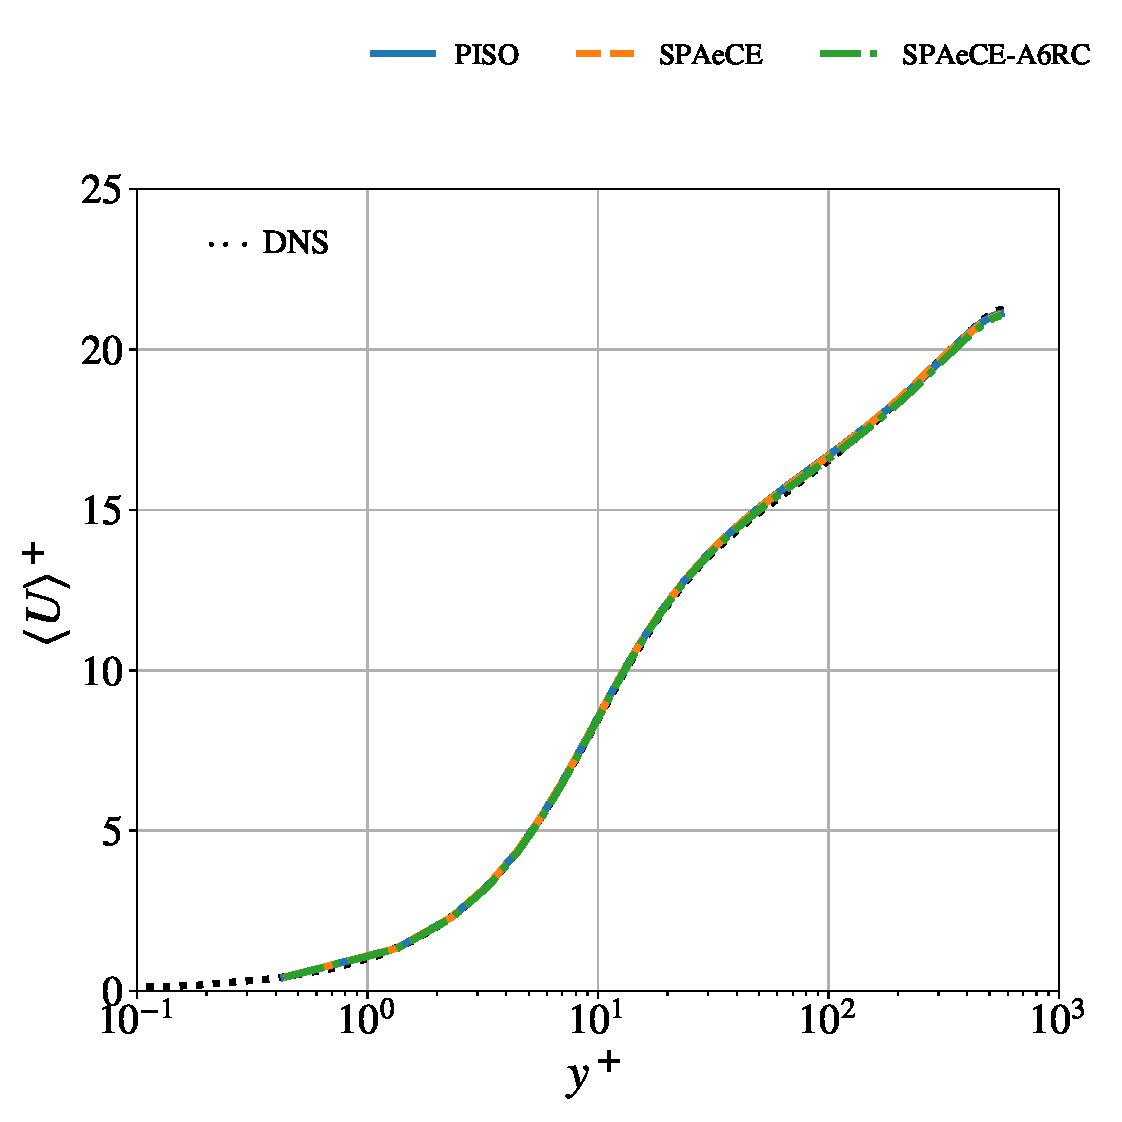
\includegraphics[width=\imgHalfWidth\columnwidth]{channel590/129x129x129/plots/PISOvsSPAeCEvsA6RC/ChannelFlowRe590_cyclic_dynKEqnHeinz_129x129x129-Uf-log.pdf}\label{fig:channel590-Cart129-MeanStreamwiseVelocity}}
\subfloat[Mean shear stress]{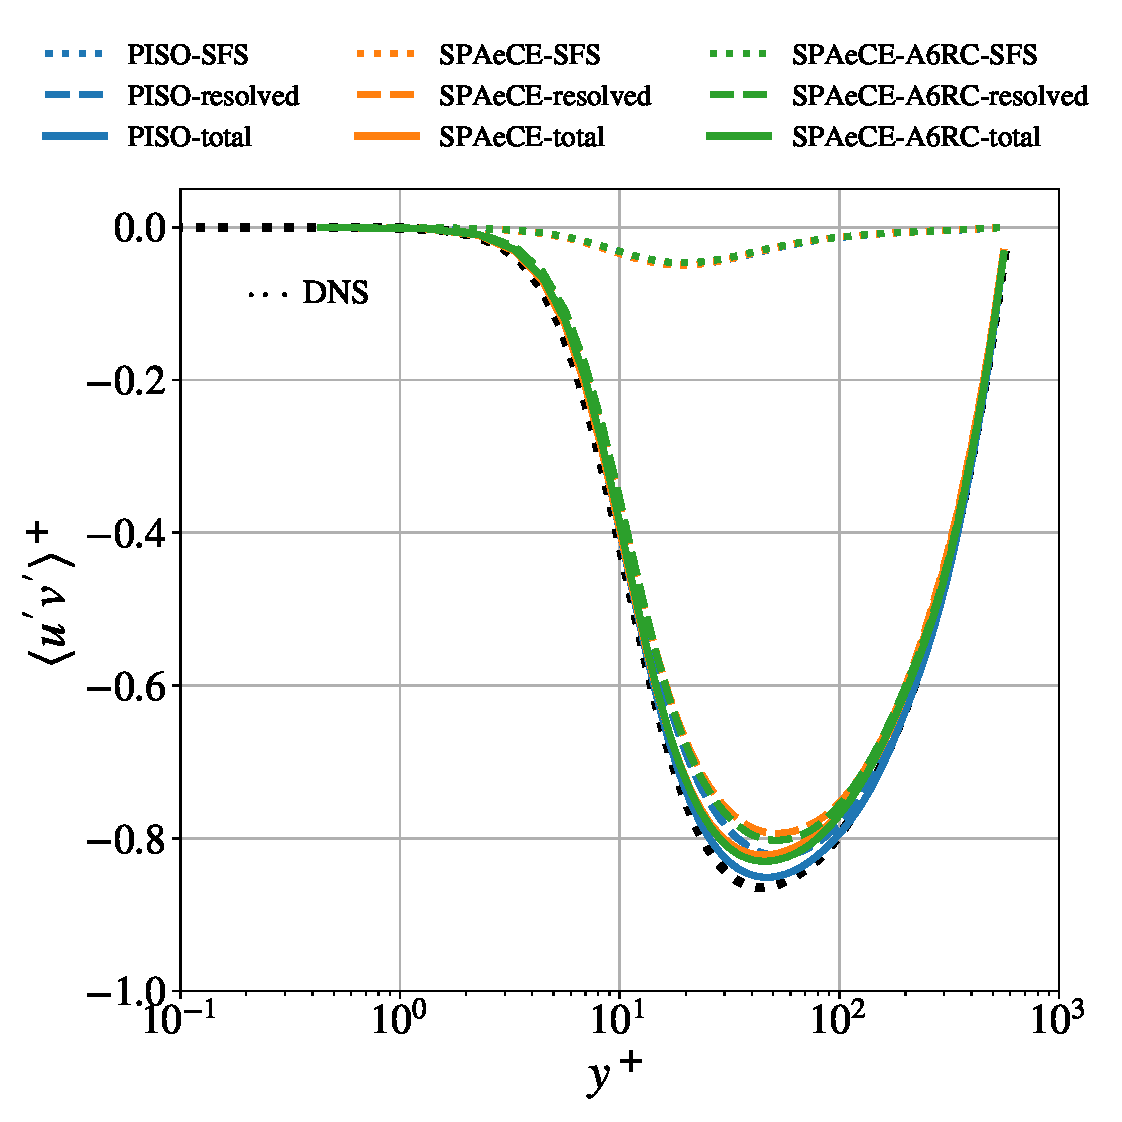
\includegraphics[width=\imgHalfWidth\columnwidth]{channel590/129x129x129/plots/PISOvsSPAeCEvsA6RC/ChannelFlowRe590_cyclic_dynKEqnHeinz_129x129x129-uv-log.pdf}\label{fig:channel590-Cart129-MeanShearStress}} 
\caption{Mean stream-wise velocity and shear stress comparison among the \piso, \spaece and \spaeceARC algorithms in a fully developed channel flow at $Re_\tau = 590$ simulated in a Cartesian hexagonal $129 \times 129 \times 129$ mesh} 
\label{fig:channel590-Cart129}
\end{figure}


The mean streamwise velocity and shear stress comparison is illustrated in Fig. \ref{fig:channel590-Cart129} and compared with DNS profiles derived by Moser et al. \cite{moser1999}. The flow is initialized from a 2D RANS simulation and random perturbation is introduced to facilitate transition to 3D flow. After initial transient time of $200s$, flow statistics is gathered for $300s$. The time-averaged fields are averaged in the homogeneous stream-wise and cross-stream directions. To leverage the symmetry of the fully developed flow, the symmetric profiles averaged again. 

All three algorithms produced an exact match with DNS mean stream-wise velocity profile. The well-refined mesh results in small sub-filter-scale (SFS) stress contribution in the viscous wall region $( y^+ < 50)$ and the resolved stress is overwhelmingly large signifying the simulation transition from LES at the near-wall region $( y^+ < 100)$ to DNS at the channel center $( y^+ > 100)$.

\begin{figure}[!h]
\centering
\subfloat[$y^{+} = 5$]{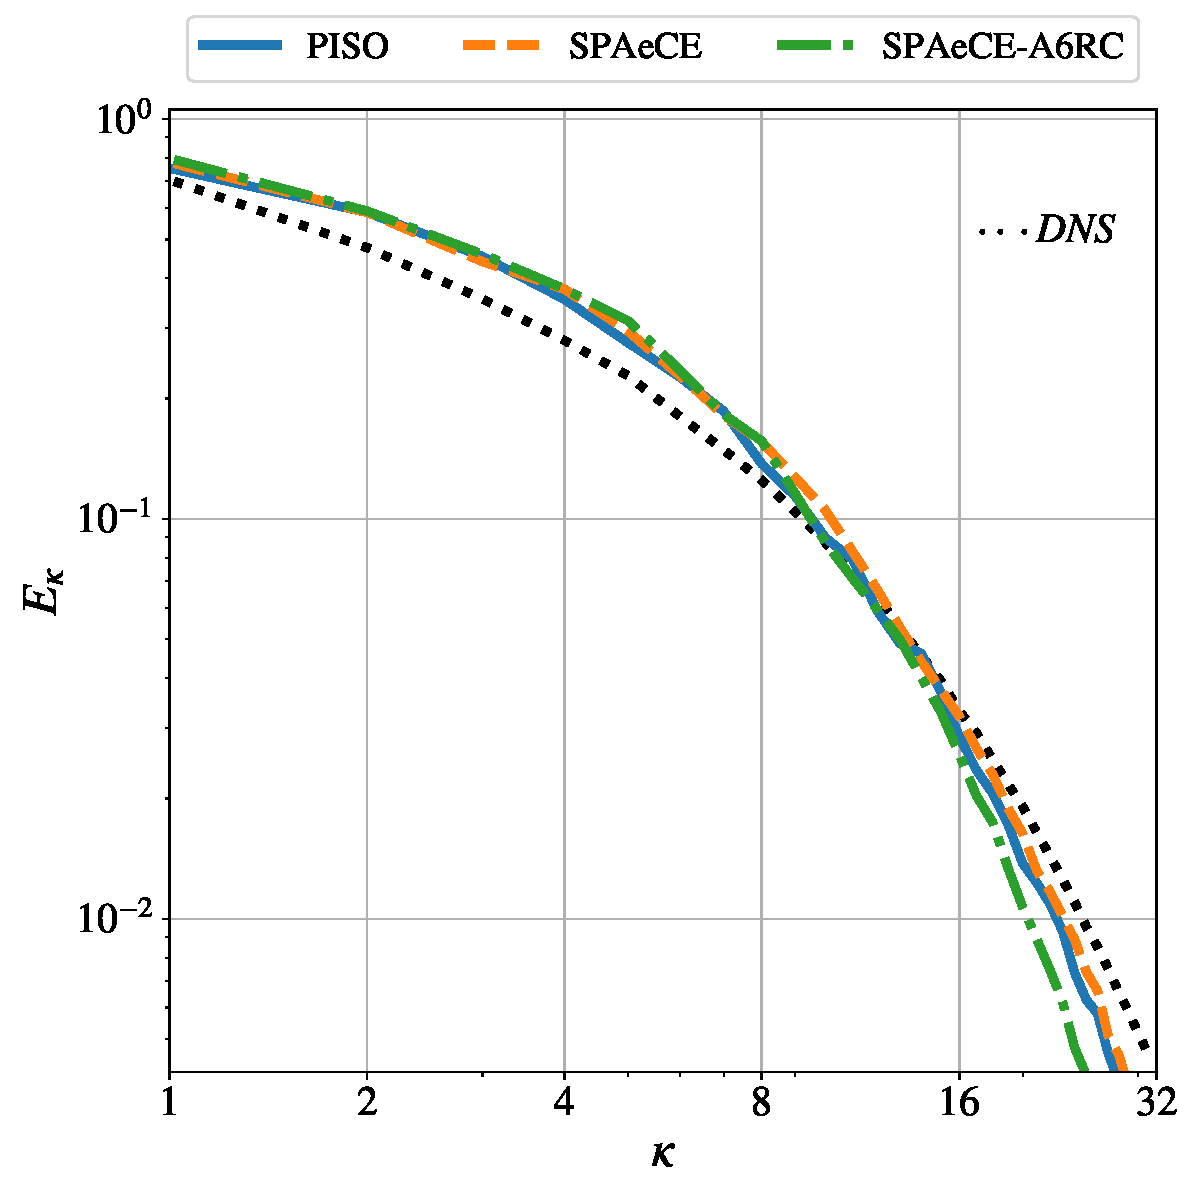
\includegraphics[width=\imgHalfWidth\columnwidth]{channel590/129x129x129/plots/specturmX/specturmX_Y5.pdf}\label{fig:channel590-Cart129-Spec5}}
\subfloat[$y^{+} = 587$]{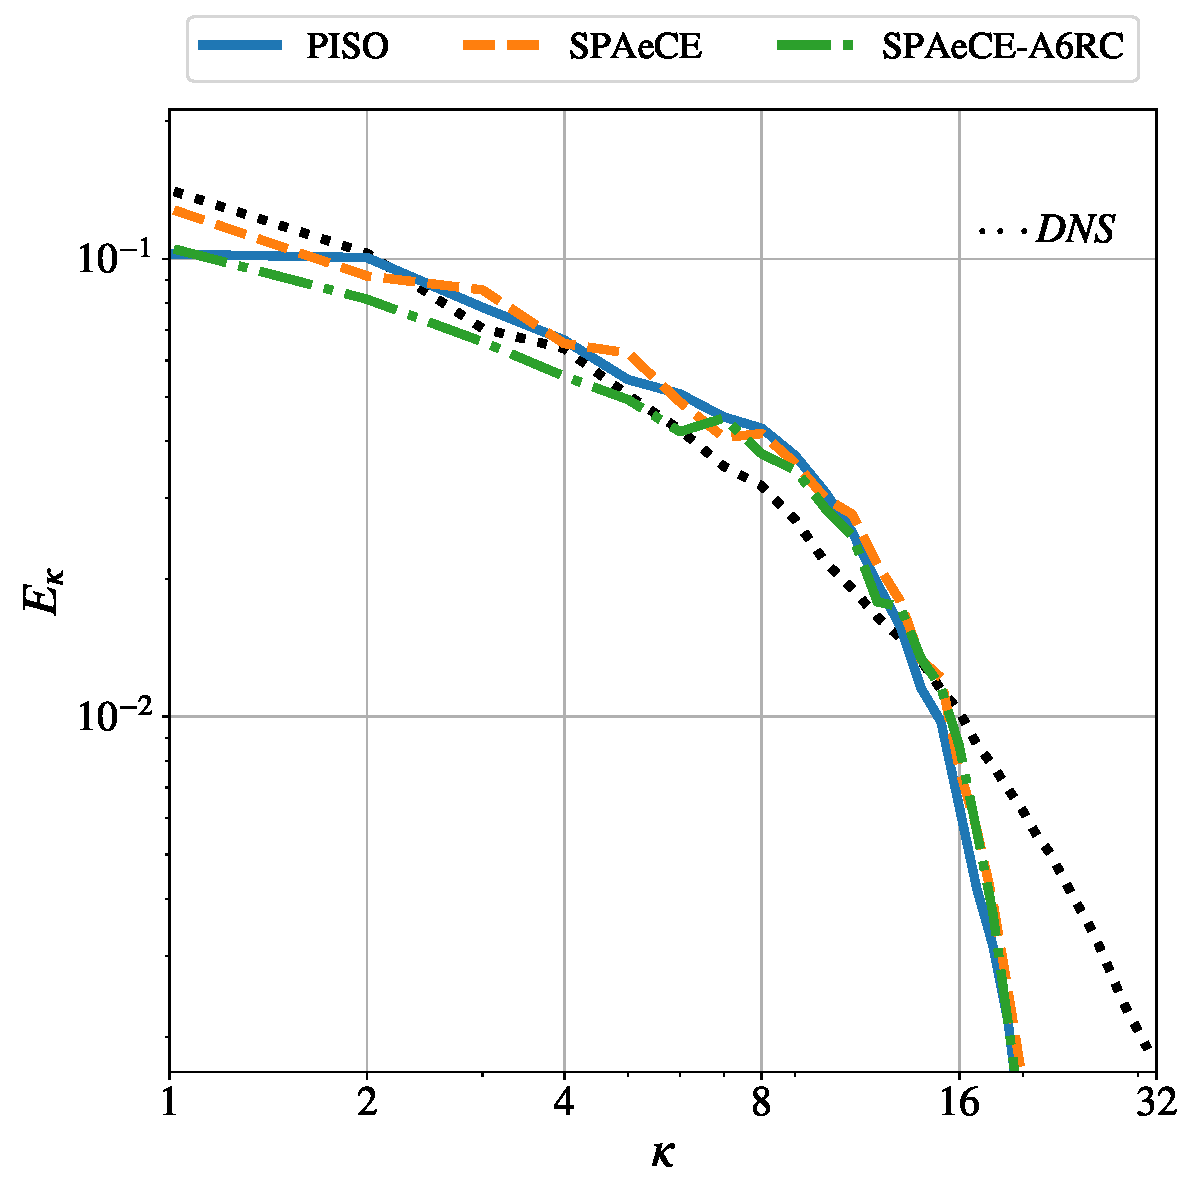
\includegraphics[width=\imgHalfWidth\columnwidth]{channel590/129x129x129/plots/specturmX/specturmX_Y587.pdf}\label{fig:channel590-Cart129-Spec587}} 
\caption{KE spectrum comparison in stream-wise direction at wall-normal heights $y^+ = 5, 587$ compared among the \piso, \spaece and \spaeceARC algorithms in a fully developed channel flow at $Re_\tau = 590$ simulated in a Cartesian hexagonal $129 \times 129 \times 129$ mesh} 
\label{fig:channel590-Cart129-Spec}
\end{figure}

KE spectrum in stream-wise direction at two wall-normal heights $y^+ = 5, \, 587$ are compared in Fig. \ref{fig:channel590-Cart129-Spec}. All three algorithms are in good agreements wit the DNS profile. KE is over predicted in low wave numbers and under-predicted in higher wave numbers. 


\subsubsection{Fully developed channel flow: wall-modeled}


\newpage
\textbf{To do list}
\begin{enumerate}
\item Once the regularization approach is finalized, compare performance among \piso, \spaece and \spaeceARC algorithms.

\item Investigate if there is any benefit of \textit{consistent} approach in Poisson pressure correction (lots of testing and validation).

\item Fully developed channel flow in unstructured grid: shall I make a hybrid grid with Cartesian cell near wall and Delauney triangulation at he core? Or a lower Reynolds number case while limiting $x^+ < 5$ to control non orthogonality?

\item Complete the wall modeled case. Review how the results vary for unstructured, non-orthogonal mesh.

   

\end{enumerate}
\chapter{Bolund Hill}

\section{abstract}
The recent proliferation of wind energy led in an increased penetration of wind farms in complex terrains. Unlike simple terrains, near surface wind experiences high variation in velocity and enhancement of turbulence in the complex terrains. Local measurement in sparse locations is inadequate to assess such diverse wind profile and application of numerical models has the potential to deliver detailed insight. In this work, the Bolund hill experiment, a rigorous complex terrain field campaign, is used to validate a Large Eddy Simulation (LES) model. The LES model applied is available in the SOWFA solver library developed based on the open-source solver OpenFOAM. A series of precursor LES has been performed to bridge the gap between atmospheric macro scale with terrain induced micro scale and used as a source of turbulent inflow for the Bolund hill LES. The influence of turbulent inflow is compared with a steady inflow LES. The sequential precursor LES found consistent in terms of mean velocity and turbulence stresses. Although, minor differences found for mean wind speed, the TKE of the steady inflow Bolund hill LES is always under-estimated. The precursor inflow fed Bolund hill  LES performed well in areas of nearly flat terrain and have a few scope of improvements in the difficult flow regions such as steep slope and ridges. Due to computational resource limitation, only two hill LES with different turbulent inflow for ten minutes each has been performed, which is statistically inadequate compared to enormous data compiled in the experimental campaign. This study identified the importance of turbulent inflow for complex terrain LES  and established a feasible and optimal approach to generate turbulent inflow through sequential precursor LES. Bolund hill LES resulted in some encouraging results and we identified the areas which need a more careful investigation to improve the overall prediction.


\section{Introduction}
\label{sec:1}

In recent years, the proliferation of wind energy led to the erection of wind farms in complex terrains to take benefit from better wind resources. Complex terrain substantially affects wind velocity and turbulence characteristics particularly in the near-surface region and around bluff bodies. Speed up of mean wind is often found with significant enhancement in turbulence. Hence, good knowledge of wind flow over complex terrains is essential to evaluate wind energy potential, assess structural loads, determine wind turbine design and sitting, and ultimately derive wind farm economics. Measurement from meteorological towers in sparse locations is essential, but not sufficient to reflect the intricate wind profile in complex terrains. Numerical models have the potential to offer insight with high fidelity information in this regard.

Wind flow in complex terrains exhibits diverse phenomenon ranging from flow stagnation, rapid acceleration-deceleration, recirculation-reattachment, vortex shedding, etc. Such micro-scale events occur at higher frequencies (as well as at smaller spatial scales) compared to meteorologic synoptic scale events. To resolve these flow features, the numerical models have to operate in a time accurate manner along with grid resolution in the order of length-scale of these 

Turbulence models like Reynolds Averaged Navier-Stokes (RANS) models are very economical to operate, however, only provide statistically averaged solution. Besides, they are known to be inaccurate in the flow separation-recirculation zones. The Large Eddy Simulation (LES) models provide a viable alternative, which provides an accurate prediction with the trade-off of higher computational cost. LES models only resolve relatively large-scale events and mathematically model the smaller scales, thus can be set to capture flow structures evolving around the complex terrains. Prior to the application with confidence, irrespective of category, any turbulence model need to be validated against experimental measurements.

Over the past three decades, following wind farm sitting in simple terrains, various atmospheric boundary layer flow experiments were performed on terrains with gentle slopes. The main focus of these studies was to derive mean wind profile and turbulence intensity, whereas insight into terrain and flow turbulence interaction was limited. This was partly due to most of the available numerical models was either linear or RANS type model, which do not produce information regarding turbulence structures. 

With growing penetration of wind farms in complex terrains, accurate and high-fidelity information of complex wind flow became important. In recent years, due to the abundance of inexpensive computational resources, application of LES models become feasible. LES models can reproduce spatio-temporally varying turbulent flow, thus higher order and spectral analysis can be performed which is important to understand the effect of turbulence on wind turbine structures. Despite encouraging potentials, performing LES is challenging, because of difficulties in sub-grid-scale model applied (to account for small turbulent scales), specifying appropriate boundary condition particularly the inflow condition, treatment of rough terrain surface, etc. The ``Bolund Experiment''\cite{Berg2011} is a benchmark case for atmospheric boundary layer flow over complex terrain and considered as the validation test case in this study. A LES model from the open-source SOWFA \cite{Churchfield2012, Churchfield2013} solver library is used to reproduce the experimental campaign over the Bolund hill. The experiment description, review of the previous validation studies and details of the current LES model validation are elaborated in the subsequent sections.


\section{The Bolund Hill experiment}
\label{sec:2}

\subsection{Topology}
\label{subsec:2.1}

The experimental campaign is performed on an isolated hill in Bolund Peninsula, located north of Riso campus of DTU in Roskilde Fjord, Denmark during three winter months of 2007-2008\cite{BolundProjectWeb}. The Bolund hill is a naturally formed island of an approximate dimension of $150 m$ length in the west-east direction, $100 m$ width in the south-north direction, and $11 m$ in height. The hill is mostly flat and surrounded by a narrow beach. On the west side, it has an almost vertical escarpment with some overhanging portion. The other sides have a moderate slope with rounded crest. Being located in a bay, the hill is ringed by water in all except east direction where a narrow isthmus connects the hill with the mainland. The figure \ref{fig:contour} depicts a contour map of the Bolund hill terrain and measurement mast locations.

%
\begin{figure}
    \centering
    \includegraphics[width=0.75\textwidth]{./contour-wMast.png}
    \caption{Countour map of the Bolund hill in 0.25m interval. The masts (marked in red dots) are located along two transects A and B. The mast M3 denotes the center point of the hill [image reproduced from Bechmann et al. \cite{Bechmann2011}] \label{fig:contour}}
\end{figure}
%

The Bolund hill center is defined arbitrarily on top of the hill to serve as the local reference, which is also the position of mast M3. The measurement mast M0 is placed approximately 181 m west, 100 m south of hill center out at sea (on a floating platform). On the Bolund hill, measurement masts are placed along two lines to capture flow from two predominant wind directions. Four masts (M1, M2, M3, M4) are aligned with Line A with an angular orientation of $239^o$ and four more masts (M3, M6, M7, M8) forms the Line B of $270^0$ angle. The mast M5 is placed in the due south on the beach and mast M9 is placed approximately $327 m$ east and $39 m$ south on a small beach, which is south of the isthmus.

For ease of simulation, only the westerly wind ($270^0$) is considered for the validation study. The mast M0 is assumed to be placed in sufficient upstream distance to measure the incoming wind profile. The mast M9 will serve to examine downstream wind affected by the bluff shape of the hill. On each mast, multiple anemometers (cup/sonic) are placed at different heights to record the wind profile. Two temperature probes at different height were placed on each mast M0 and M9 to determine the atmospheric stability condition. In the experiment, data sets are collected at $20 Hz$ sampling rate in $10$ minute blocks for all probes. For the current study, data sets with average wind speed exceeding $5 m/s$ and $|1/L_{MO}| < 0.004 m^{-1}$ have been selected for validation, where $L_{MO}$ is the Monin-Obukhov length (eq. \eqref{eq:MO}). 

The westerly wind experiences an approximately $7\, km$ fetch over the calm bay which is characterized by a small roughness height of 0.0006 m \cite{Berg2011}. Such near-perfect incoming flow condition provides a well-defined quantitative description of incoming flow and it is crucial for boundary condition implementation in the numerical models. Except for the sandy beach and near-vertical escarpment, the Bolund hill is mostly covered with grass and characterized by a uniform roughness length of 0.015 m \cite{Berg2011}. In the field experimental campaign, a maximum 30 \% speedup is found associated with 300 \% enhancement of turbulence intensity \cite{Berg2011}. It implies that the best site for the erection of wind turbines to maximize energy harness have to bear a penalty of increased structural fatigue loads. For the westerly wind, the Bolund hill also features a transient recirculation zone at the escarpment edge and downstream flow deceleration in the eastern slope.

%
%
%
\subsection{Scale effects}
\label{subsec:2.2}
%
The physical shape of the Bolund hill represents a scaled down form of a typical wind turbine site in complex terrain. Hence, computational resources required for Bolund hill simulation will be much smaller than a realistic complex terrain e.g. a mesa hill. However, the scale effects shall be accounted before inferring any decision made from Bolund hill simulation. Berg et al. \cite{Berg2011} suggested a typical mesa hill of $10-30$ times in all dimensions and aerodynamic surface roughness length.

According to S. Pope \cite{pope2000tf}, Reynolds number similarity implies Reynolds number independent flow solutions and is essential for turbulence models such as LES. In the present study, Reynolds number is defined based on the hill height $h$ and the free-stream velocity $U$. For Bolund hill with $U \approx 10 m/s$, $Re_{Bolund} \approx 10^7$ and for the same characteristic velocity over the mesa hill, $Re_{mesa} \approx 10^8$. Lim et al. \cite{Lim2009} conducted a series of wind tunnel experiments of flow over bluff bodies in a turbulent boundary layer with concentrated vortex motion and studied flow Reynolds number up to $10^6$. Even at such high Reynolds numbers variation observed in surface pressure and near surface speed with the change of Reynolds number. Although the Bolund and mesa hill Reynolds numbers are even higher of a different flow type, the Reynolds number dependence cannot be ruled out completely.

Influence of atmospheric stability and boundary layer height $z_i$ is also important when scaling up Bolund to the mesa hill. The Monin-Obukhov length determines the height of significant surface influence within the boundary layer and defined as
%
\begin{equation}
\label{eq:MO}
 L_{MO} = - \frac{u_{*}^3}{\kappa (g/ \theta) \overline{w^\prime \theta^\prime}},
\end{equation}
%
where the friction velocity is defined by $u_* = \left[ \overline{u^\prime w^\prime} + \overline{v^\prime w^\prime}\right]^{1/2}$. Here, $u\, v \, w$ are the averaged axial, lateral and vertical components of the wind velocity vector respectively, $\theta$ is the potential temperature and the primed quantities are fluctuations around these values. The $\overline{...}$ represents the ensemble average operator. $\kappa=0.4 $ denotes the von-Karman constant and $g$ is the gravitational acceleration constant.

For Bolund experiment, the hill height is much smaller than the temperature inversion height (boundary layer depth) $z_i$ and the Monin-Obukhov length $L_{MO}$. Therefore flow perturbations induced by the bluff hill expected to dominate over perturbations caused due to atmospheric instability \cite{Berg2011}. So irrespective of atmospheric stability condition, the atmosphere can be approximated as neutral. However, such assumption may not be applicable for the mesa hill. In a neutral atmosphere with high wind speed or in an unstable atmosphere where boundary layer height $z_i$ is very high, stability effects can be neglected. In the case of the stable atmosphere, where the boundary layer depth $z_i$ is usually low (comparable to mesa hill height), strong effects of stratification are expected and generalization from Bolund to mesa hill fails \cite{Berg2011}. In the current study, experimental measurements recorded only in a neutral atmosphere are used for LES model validation.

The influence of Coriolis force shall be accounted as well. For vertical direction, the Ekman depth has an approximate size of atmospheric boundary layer height. Thus, change of wind direction with height may influence the mesa hill flow at least in a stably stratified atmosphere. The height of Bolund hill is much smaller than the Ekman depth and hence Coriolis effect in the vertical direction can be neglected. To estimate influence in horizontal direction, the Rosby number ($Ro = U/fL$, where $f \approx 10^{-4} s^{-1}$ for mid-latitudes has been taken into account. For Bolund hill, $Ro \approx 660 >> 1$ and Coriolis effect on the wind can be overlooked. On the other hand, for mesa hill, $Ro \approx 60 > 1$ and Coriolis effect may become significant. Therefore, numerical simulation of Bolund hill can be performed for the neutral atmospheric boundary layer without accounting for the Coriolis force effect. 


\section{Previous validation studies}
\label{sec:3}

To date, a number of RANS and LES simulations have been performed for the Bolund Experiment. During 2009, a blind comparison workshop was organized to compare 88 different validation studies performed with physical models as well as various types of linear and CFD simulation models \cite{Bechmann2011}. A few more  studies have also been published since then.

In terns of mean velocity speedup, the RANS models produced a $10-20\%$ error on average (Berg et al. 2 eq. $15.1\%$ \cite{Berg2011}, Berg et al. 1 eq. $17.2\%$ \cite{Berg2011}, Prosthaopoulos et al. $10.3\%$ \cite{Prospathopoulos2012}). For the turbulent kinetic energy (TKE), the error is about $50 \%$ (Berg et al. 2 eq. $47\%$ \cite{Berg2011}, Berg et al. 1 eq. $45\%$ \cite{Berg2011}. Prospathopoulos et al. concluded that RANS models can not reveal the small-scale intermittent behavior such as flow recirculation over the edge of escarpment-top \cite{Prospathopoulos2012}.

On the other hand, some LES models demonstrated slight improvement over the RANS models. Deviation of the mean velocity is found in the range of $10-20\%$ (Conan et al. $11\%$ \cite{Conan2015}, Diebold et al. $12.1\%$ \cite{Diebold2013}, Bechmann et al. $17.3\%$ \cite{Bechmann2011}) and for TKE in $20-50\%$ (Conan et al. $20\%$ \cite{Conan2015}, Bechmann et al. $48\%$ \cite{Bechmann2011}). 
Significant deviations were mainly observed in the near-surface regions and the prediction got better at higher elevations.
 
Prescribing the appropriate turbulent inflow is crucial and challenging for atmospheric boundary layer simulation. In the case of RANS models, average velocity and turbulence parameters (e.g. TKE) are prescribed for the inlet boundary condition. However, LES models require realistic spatio-temporally varying turbulent inflow. Precursor simulations and boundary layer recirculation (also called recycling method) \cite{Conan2015,Vuorinen2015} are commonly used methods to generate turbulent inflow for LES simulations.

In terms of mesh generation, two approaches are being mostly used. The terrain following meshing approach uses cells that follow the terrain surface and extrude in the vertical direction. From a meshing perspective, preparation of a terrain-following mesh over complex topography is challenging but provides the option to resolve the near-surface boundary layer and was applied in simulations performed by Conan et al.\cite{Conan2015} and Bechmann et al.\cite{Bechmann2011}). The other approach is the Immersed Boundary Method (IBM), which superimposes the terrain surface into a Cartesian grid and solves for the computational cells above the terrain only (e.g. Jafari et al. \cite{Jafari2012}, Diebold et al.\cite{Diebold2013}). Mesh generation in IBM is fast and usually require fewer grid cells. However, its' capacity to resolve the near-surface boundary layer is somewhat limited. 

Since the terrain surface is rough, the flow boundary layer can't be resolved down to the surface. In practice, wall models are used to prescribe shear stress at the surface to reproduce the logarithmic law of wall region of the mean boundary layer velocity profile. The accuracy of the wall model is important particularly in regions of abrupt surface roughness change (here calm sea and grass covered hill)) and flow separation-recirculation. In the case of complex terrain, local flow variation is present in smaller spatial and temporal scale compared to typical simple terrain simulations and so a finer mesh resolution is recommended (Berg et al. \cite{Berg2011}).

\section{LES model description}
\label{sec:4}

In this work, the Simulator for On/Offshore Wind Farm Applications (SOWFA) which is an OpenFOAM \cite{weller1998OpenFOAM} based solver library developed at the U.S. Department of Energy’s National Renewable Energy Laboratory (NREL)\cite{Churchfield2012, Churchfield2013} is used for the Bolund hill simulation. SOWFA is based on the incompressible Navier-Stokes equations for atmospheric/wind farm large-eddy simulation (LES) that incorporates the Boussinesq approximation for buoyancy and adopts a PIMPLE (PISO/SIMPLE) algorithm for the pressure-velocity coupling. 

The governing equations for mass conservation is
%
\begin{equation}
\label{continuty}
\ddx{\Ua{i}}{i} = 0,
\end{equation}
%
and the momentum conservation equation is
%
\begin{equation}
\label{momentum}
\ddt{\Ua{i}} + \ddx{\Ua{i} \, \Ua{j}}{j} = - \frac{1}{\rho_0} \ddx{\av{p}}{i} + \rho_b g_i - \ddx{\tau_{ij}}{j} -2 \epsilon_{i3k} \Omega \Ua{k},
\end{equation}
%
where viscous fluxes are neglected due to the hign Reynolds numers of ABL flow. The energy conservation equation can be expressed as the potential temperature transport equation and expressed as
%
\begin{equation}
\label{potTemp}
\ddt{\av{\theta}} + \ddx{\Ua{j} \, \av{\theta}}{j} = - \ddx{\tau_{\theta i}}{i}.
\end{equation}
%

In the governing equations above, the overline $\av{...}$ denotes the LES filtering operator and $\Ua{i}$ is the component of the resolve velocity vector in the $x_i$ coordinate direction. The modified pressure is considered as the deviation from the hydrostatic pressure $p = p - \rho_{0}gh$ where $\rho_{0}=1$ is a reference density which is constant in the flow. The Boussinesq approximation considers density as a variable only in the gravitational term. Here, $\rho_b$ is a scalar that dictates the sign and strength of the buoyancy force and computed by 
%
\begin{equation}
\label{rhoB}
\rho_b = 1 - \beta \left(\av{\theta} - \theta_0 \right) = 1 - \left( \frac{\av{\theta} - \theta_0}{\theta_0} \right),
\end{equation}
%
where $\beta$ is the thermal expansion coefficient, $\av{\theta}$ is the resolved scale potential temperature and $\theta_0$ is a reference temperature. The term $2 \epsilon_{i3k} \Omega \Ua{k}$ accounts for Coriolis effect where $\epsilon_{i3k}$ denotes the alternating unit tensor, $\Omega$ is the planetary rotation rate vector at the point of interest on the planet (a latitude dependent quantity) and $g_i$ is the gravitational constant vector.

In LES, the sub-grid-scale (SGS) stress $\tau_{ij}$ and SGS temperature flux $\tau_{\theta i}$ quantities are modeled. The SGS values are usually multiple order of magnitude larger than molecular viscosity/diffusivity and ignored in this LES model. The majority of turbulence models rely upon the linear eddy-viscosity (Boussinesq) assumption that relates the SGS stress to the resolved-scale strain by
%
\begin{equation}
\label{sgsStress}
\tau_{ij}^D = -2 \nu_t \av{S}_{ij},
\end{equation}
%
where $\nu_t$ is the turbulence/eddy viscosity, $\tau_{ij}^D$ is the deviatoric part of the SGS stress and $\av{S}_{ij} = \half \left( \ddx{\Ua{i}}{j} + \ddx{\Ua{j}}{i} \right)$ is the resolved scale strain. Similarly, the SGS temperature flux can be expressed as
%
\begin{equation}
\label{sgsTempFlux}
\tau_{\theta i} = -\frac{\nu_t}{Pr_t} \ddx{\av{\theta}}{i},
\end{equation}
%
where $Pr_t$ is the turbulent Prandtl number. Following the equations \eqref{sgsStress} and \eqref{sgsTempFlux}, the $Pr_t$ is a flow specific parameter which must be prescribed and the eddy viscosity $\nu_t$ have to be defined. Smagornisky \cite{smagorinsky1963LES} devised one of the earliest model for $\nu_t$:
%
\begin{equation}
\label{Smagornisky}
\nu_t = \left(C_s \av{\Delta} \right)^2 \av{S}, \quad \av{S} = \left(2 \av{S}_{ij} \, \av{S}_{ij} \right)^\half,
\end{equation}
% 
where $C_S$ is a model constant, $\av{\Delta}$ is the characteristic LES filter length tied to mesh resolution. Here we adopt the Lagrangian averaged scale invariant dynamic Smagornisky model of Meneveau et al.\cite{MeneveauLagDynSGS1996}. The model constant is calculated as in the conventional dynamic Smagorinsky model
%
\begin{equation}
\label{CsModelAvg}
C_s^2 = \frac{\avT{ M_{ij} L_{ij}}} {\avT{M_{kl} M_{kl}}},
\end{equation}
%
but the averaging is performed along flow streamlines and the averaged quantities are called $\mathcal{I}_{LM} = \avT{ M_{ij} L_{ij}}$ and $\mathcal{I}_{MM} = \avT{ M_{kl} M_{kl}}$. The averaging is achieved by solving transport equations
%
\begin{equation}
\label{ILM}
\ddt{\mathcal{I}_{LM}} + \av{U}_j \ddx{\mathcal{I}_{LM}}{j} = \frac{M_{ij}L_{ij} - \mathcal{I}{LM}} {\theta^* \av{\Delta} \left(\mathcal{I}_{LM} \mathcal{I}_{MM} \right)^{-1/8} },
\end{equation}
%
and 
%
\begin{equation}
\label{IMM}
\ddt{\mathcal{I}_{MM}} + \av{U}_j \ddx{\mathcal{I}_{MM}}{j} = \frac{M_{ij}M_{ij} - \mathcal{I}{MM}} {\theta^* \av{\Delta} \left(\mathcal{I}_{LM} \mathcal{I}_{MM} \right)^{-1/8} },
\end{equation}
%
where $\theta^* = 1.5$ is a model constant. The Smagorinsky constant $C_S$ values are bounded between $0.07-0.14$ in this study.


Because of the rough terrain surface, LES models can't resolve the viscous sub-layer, instead, wall models are used to prescribe shear-stresses where the computational node (cell-center or vertices) next the surface is placed in the logarithmic region of the boundary layer. The Schumann-Grotzbach model \cite{Schumann1975,Grotzbach1977} is used to specify surface-normal shear stresses and all other components are set to zero. The SGS stress at the wall is expressed as
%
\begin{equation}
\label{SchumannGrotzbach}
\tau^{wall}_{ij} =\left\{ \begin{array}{ll}
 -u^2_* \frac{\av{U_i}(z_1)}{\vert \avT{\av{U_i}(z_1)} \vert},& \mbox{i= 1,2; j=3,} \\
 0, & \mbox{otherwise.}\end{array} \right.
\end{equation}
%
where it is assumed that $i=1,2$ refers to the surface parallel coordinates and $j=3$ refers to the wall normal coordinate.


\section{LES simulation results}
\label{sec:5}

\subsection{Generation of turbulent inflow data}
\label{subsec:5.1}

Flow behavior in a time-resolved simulation such as LES is influenced by boundary conditions, particularly by the inflow condition. Flow turbulence can be described in terms of pseudo-random coherent motions of a wide range of spatial and temporal scales superimposed on some “mean flow” \cite{Tabor2010LesInflow}. In the case of atmospheric boundary layer flow, larger flow scales are determined by meteorologic synoptic events or the terrain geometry (e.g. surface features) and the smallest scales are determined by fluid viscosity. Since LES resolves the relatively large-scale fluid motions only, simulation inflow must bear relevant flow scales in a coherent manner. The precursor simulation method is a well-known approach, where a separate LES of an equilibrium turbulent flow is performed to generate a library of turbulent flow data which can be introduced as inflow to another LES. Precursor data library can preserve turbulence scales with proper spatial and temporal correlation, and correct turbulence kinetic energy spectrum.

In the current study, westerly wind ($270^0$) in a neutral atmospheric boundary layer is investigated. A precursor simulation of dimension $L\times W\times H = 3000 m \times 3000 m \times 1000 m$ with a flat terrain of recommended calm sea surface roughness of $z_{0} =0.0006 m$ is performed. The domain is aligned in $+x$ as the east, $+y$ as the north and $+z$ as the vertical direction. Coriolis forces have been neglected as discussed in section \ref{subsec:2.2}. In the horizontal plane, a uniform grid resolution of $\Delta x = \Delta y = 10 m$ is applied. In the vertical direction, near surface resolution is kept $\Delta z_{terrain} = 5 m$ which gradually grows up to $\Delta z_{max}= 15 m$ at the top-most edge. The whole precursor Cartesian grid consists of $300 \times 300 \times 100 = 9 \times 10^6$ hexahedral cells. The east-west and north-south boundary pairs are considered as periodic for all variables. The Schumann-Grotzbach model \cite{Schumann1975,Grotzbach1977} for wall shear stress is applied to the surface and the required velocities at the first cell centers are averaged horizontally to estimate the ensemble averaged velocity. Due the use of a stress BC at the surface, specifying a surface velocity is not strictly necessary but the test filtering method used in the dynamic model relies o surface velocity values. Following the SOWFA standard, the velocity at the surface is obtained by linear extrapolation from the 1st and 2nd cell-center values. Flux-based boundary conditions are applied for velocity $\mathbf{U}$ and modified pressure $p_{rgh}$ in the top boundary which allows for inflow and outflow across the boundary. All other variables are declared as ``zero'' gradient Neumann condition at the top boundary.

The velocity field is initialized with some periodic perturbations superimposed on a mean velocity profile prescribed based on the logarithmic law of the wall. A constant potential temperature of $288K$ is prescribed throughout the domain. The \textit{ABLSolver} from the SOWFA \cite{Churchfield2012, Churchfield2013} library is used to execute the simulation for $17,000 s$ to achieve flow equilibrium and then velocity field is recorded as sample-planes in the east boundary for $2,000 s$ to build the turbulent inflow library. In these planes, vertex values of the instantaneous velocity are stored which are obtained by a linear interpolation from the face centers and the BC. 
%
\begin{figure}[htb]
\centering   %%% not \center
	\subfloat[Instantaneous streamwise velocity $U_x$]{\label{fig:CP-Domain}\includegraphics[width=0.55\textwidth]{CoarsePre/precursorVelocity_2.png}}
	\quad
	\subfloat[$U_x$ at $Z_{agl} = 500 m$ plane]{\label{fig:CP-Slice}\includegraphics[width=0.35\textwidth]{CoarsePre/Ux_500m_17000s_newcolorscale.png}}
\caption{Precursor simulation over a flat-homogeneous terrain of surface roughness $z_{0} =0.0006 m$.}
\label{fig:CP}
\end{figure}
%

Figure \ref{fig:CP-Domain} illustrates the instantaneous streamwise velocity $U_x$ field of the precursor domain where complex-correlated turbulent flow structures are evident and the figure \ref{fig:CP-Slice} depicts the instantaneous streamwise velocity in a plane $500m$ above the ground ($Z_{agl} = 500 m$). Here, the presence of very long (almost as long as the domain) alternating high and low-velocity streaks are observed. One possible reason for such features could be that the precursor domain is not long enough to allow decorrelation of these very long structures which are cycled back to the domain due to the periodic boundary condition in the streamwise direction.

Fang et al. \cite{Fang2015} conducted a neutral ABL simulation of dimension $L\times W\times H \approx 100,000 m \times 12,500 m \times 1000 m$. The authors observed that the majority of the flow streaks are larger than $5,000m$ (which is larger than present domain extension). They also discovered the presence of very large-scales motions (VLSMs) as long as $20,000 m$ in streamwise and $500 m$ in cross-stream direction. The contribution of structures larger than $10,000 m$ to the resolved kinetic energy and shear stress are found to be up to $27$ and $31\%$ respectively, which is significant. Hence, use of a precursor domain of such large size in the present study seems necessary but infeasible due to enormous computational cost involved. 

The vertical grid resolution of the precursor domain is in the range of $5-15 m$, which also indicates the lower limit of the turbulence structures resolved by the precursor simulation. Since the Bolund hill is about $11m$ high, relatively finer turbulence structures are necessary to observe flow turbulence and hill geometry interaction. Hence, a second precursor simulation with finer resolution is performed using the inflow library from the preceding ``coarse'' precursor and is termed ``fine'' precursor hereafter.

The fine precursor domain has a dimension of $L\times W\times H = 500 m \times 500 m \times 200 m$ with horizontal resolution of $\Delta x = \Delta y = 2m$ and a vertical resolution ranging from $\Delta z_{terrain} \approx 1 m$ (at the surface) to $\Delta z_{max} \approx 4 m$ (at the top). The Cartesian mesh consists of $250 \times 250 \times 100 = 6.25 \times 10^6$ hexahedral cells which are overall about $5$ times smaller in each dimension than the coarse precursor cells. The domain alignment and surface roughness remained unchanged. The flow field variables are initialized from the coarse precursor fields and time-varying turbulent inflow velocity from the coarse precursor is prescribed on the inflow (west) boundary. The recorded instantaneous velocity at the vertices of the coarse precursor is linearly interpolated in space to the fine precursor inlet face centers. Linear interpolation is also used for time as the fine precursor uses a much smaller time step than the coarse precursor. 

The velocity boundary condition at the outflow (east) boundary is specified as ``zero'' gradient Neumann condition and the modified pressure $p_{rgh}$ is prescribed as fixed value ``zero'' Dirichlet condition. A filtered flux-based boundary condition for $\mathbf{U}$ and ``zero'' gradient condition for $p_{rgh}$ is applied in the north, south and top boundaries. Boundary conditions for the surface are kept same as in the coarse precursor. 

The fine precursor contains several cells within one coarse precursor cell (cell center located at $Z_1^{coarse}$). When the inflow data from the coarse precursor is interpolated to the fine precursor inlet face centers, the surface velocity of the coarse precursor would be the lowest value for the linear interpolation and the upper value would correspond to the value obtained from the top face center of the first coarse precursor cell. However, the surface velocity in the coarse precursor is obtained by a linear extrapolation from the 1st and 2nd cell-center values in the surface normal direction and thus does not follow a logarithmic law. Hence, simple linear interpolation of the coarse precursor inflow data will lead to a large error. To avoid this issue, a modified interpolation process is introduced and portrayed in the figure \ref{fig:PreInterp}. 
%
\begin{figure}[htb]
\centering   %%% not \center
	\includegraphics[width=0.5\textwidth]{CPvsFP/PrecursorVelInterpolation.png}
\caption{Modified linear interpolation for coarse to fine precursor projection in the near-surface region}
\label{fig:PreInterp}
\end{figure}
%

In figure \ref{fig:PreInterp}, the ground level $Z_{abl}=0$ is marked by a hatched line and log-law of wall is marked by the solid blue line. Here, the red dashed line depicts the velocity profile approximated by the coarse precursor. If this profile is passed on to the fine precursor, all interpolated values between the surface and $Z_1^{coarse}$ will be significantly larger (e.g. red square marker) than the expected logarithmic profile following values. Hence, the surface velocity of the coarse-precursor inflow library has to be modified (magenta square marker) such that the linear interpolation will provide the correct log-law value (green square) when time averaged. In the presence of multiple cell-centers, all values will follow the modified interpolation path (dashed magenta line) which ensures less error than the primitive interpolation path (red dashed line). Thus, a better near-surface velocity profile is obtained for the inlet boundary of the fine precursor. 

In the fine precursor LES the same \textit{ABLSolver} solver is used and the simulation is first run for $200 s$ to allow for flow evolution. Then, the velocity field is recorded for $1800 s$ on the east boundary to build the second inflow library which will be modified (following the interpolation depicted in fig. \ref{fig:PreInterp}) and fed into the Bolund hill simulation later. Figure \ref{fig:FP} illustrates a comparison between the coarse (left) and fine precursor (right) results of the instantaneous streamwise velocity in a $Z_{agl} = 10 m$ plane at the same time as if they are simulated together. The coarse precursor (fig. \ref{fig:CP-Ux}) represent a plane of the same dimension of fine precursor from the $2500 m$ to west boundary ($3000 m$). The larger scale flow structures in the coarse precursor quickly introduce smaller scale structures along the downstream in the fine precursor (fig. \ref{fig:FP-Ux}). 


%\textcolor{red}{it was not clear to me how the two pictures connect together?}
 
%
\begin{figure}[htb]
\centering   %%% not \center
	\subfloat[Coarse Precursor]{\label{fig:CP-Ux}\includegraphics[width=0.46\textwidth]{CoarsePre/finePrePlaneslice_rightside_Ux_z=10m.png}}
	\quad
	\subfloat[Fine Precursor]{\label{fig:FP-Ux}\includegraphics[width=0.45\textwidth]{FinePre/z=10m_UxSlice_17400.png}}
\caption{Instantaneous streamwise velocity in the coarse and fine precursor simulation at $Z_{agl} = 10 m$ plane.}
\label{fig:FP}
\end{figure}
% 
 
%\textcolor{red}{this statement is completley wrong. Think about it and reformulate. Consider specifying what should be expected first e.g. how the modeled and resolved contributions should change and how their sum should remain constant}


For any turbulent flow, a LES model shall yield the same ensemble-averaged resolved velocity profile for different grid resolution. As the grid gets finer in a LES, more turbulence scales get resolved and proportionally less sub-grid-scales (SGS) have to be accounted though the SGS stress model. Nevertheless, the total turbulence stress (resolved + SGS) profile for different simulation irrespective of grid resolution (i.e. filter size) shall remain consistent. The figure \ref{fig:PreComp} depicts the mean streamwise resolved velocity $\avT{\av{U}_x}$, streamwise normal stress $\SGSstress{u}{u}$ and shear stress $\SGSstress{u}{w}$ from both coarse precursor and fine precursor east-outlet boundary. Since the fine precursor domain width is much smaller than the coarse precursor, the velocity and stress fields corresponding to the fine precursor inlet dimension is considered only for comparison. The mean velocity profile $\avT{\av{U}_x}$ in figure \ref{fig:PreComp-U} obtained with the two levels of precursor simulation agree very well with each other and also agree well with the logarithmic law of the wall. 

%\textcolor{red}{This paragraph also needs improvement! You kept using ``terrain region'' or ``terrain surface'' this does not make sense in a flat precursor. Just call it the surface.}

In terms of the streamwise normal stress $\SGSstress{u}{u}$ (fig: \ref{fig:PreComp-uu}), the fine precursor SGS stress is smaller and resolved stress is larger compared to coarse precursor since more turbulent scales are resolved in the fine precursor. The total turbulence stress (resolved + SGS) matches well for both precursor simulations. A similar trend is also observed for the shear stress $\SGSstress{u}{w}$, except it is under-predicted at the near terrain region ($Z_{agl} \approx 10 m$) of the coarse precursor. Overall, the LES is consistent across both precursor simulations and the fine precursor contains desired smaller turbulent scales relevant to the Bolund hill height. Using such a sequential grid refining series of precursor simulations bridge the scale gap between atmospheric macro scales with near surface micro scales. It also requires much less computational resources than running only one large ABL precursor simulation with very fine resolution.

%
\begin{figure}[htb]
\centering   %%% not \center
	\subfloat[Streamwise mean resolved vel.$\avT{\av{U}_x}$]{\label{fig:PreComp-U}\includegraphics[width=0.32\textwidth]{CPvsFP/MeanVelocity.png}}
	%\quad
	\subfloat[Streamwise normal stress $\SGSstress{u}{u}$]{\label{fig:PreComp-uu}\includegraphics[width=0.32\textwidth]{CPvsFP/Stress-uu.png}}
	%\quad
	\subfloat[Vertical velocity $\SGSstress{u}{w}$]{\label{fig:PreComp-uw}\includegraphics[width=0.32\textwidth]{CPvsFP/Stress-uw2.png}}
\caption{Mean velocity and stress comparison between coarse and fine precursor LES.}
\label{fig:PreComp}
\end{figure}
%

\subsection{Bolund Hill Simulation}
\label{subsec:5.2}
%
The computational domain considered for the Bolund hill simulation extends from $-300m$ upstream (west) to $400 m$ downstream (east) of the hill (i.e. $700m$ long in the wind-wise direction). In the crosswind direction, the domain extends from $-210m$ south to $190m$ north giving a total width of $400m$. These dimensions place the M0 and M9 masts sufficiently far from the domain boundaries. Both cross-wind boundaries are far enough from the hill to allow for streamline bending and flow evolution around the hill. The domain height is $120m$, which is about $11$ times of the maximum hill height and assumed to adequately represent the atmospheric boundary layer relevant to Bolund hill scale. The domain is aligned with the precursor domains, where the westerly wind is perpendicular to the west (inlet) boundary.
 
%
\begin{figure}[htb]
\centering   %%% not \center
	\subfloat[Terrain surface mesh]{\label{fig:surfMesh}\includegraphics[width=0.45\textwidth]{terrainMesh_wallSpacing7.png}}
	\quad
	\subfloat[Slice of volume mesh at $y=0 m$ plane]{\label{fig:volMesh}\includegraphics[width=0.45\textwidth]{maxAngle4.png}}
\caption{Mesh for Bolund hill simulation.}
\label{fig:HillMesh}
\end{figure}
%

An anisotropic hexahedral block-structured grid is prepared with the finest resolution of $\Delta x \approx 0.30 m$ and $\Delta y \approx 0.40m$ applied at the vertical escarpment. Over the rest of the hill surface, the horizontal grid spacing varies from $0.50 m \leq \Delta x, \, \Delta y \leq 0.75 m$ somewhat depending on the local terrain details. Beyond the hill, the grid is smoothly stretched to $\Delta x_{max}, \, \Delta y_{max} \approx 4 m$ at the domain boundaries. The near-terrain vertical grid resolution is set to $\Delta z_{terrain} \approx 0.15 m$ and smoothly stretched to $\Delta z_{max} \approx 5 m$ at the top boundary. Pointwise \cite{Pointwise}, a commercial software program, is used to prepare the terrain following multi-block structured mesh resulting in approximately $28 \times 10^6$ hexahedral cells. The figure \ref{fig:HillMesh} illustrates the structured surface mesh (fig. \ref{fig:surfMesh}) and a slice though the volume mesh at $y=0 m$ plane (fig. \ref{fig:volMesh}). Resolving the curvature at the vertical escarpment was challenging and a few moderately non-orthogonal cells are inevitably formed (marked by green color in fig. \ref{fig:volMesh}). The maximum non-orthogonality is around $138^o$ and the average is $5.7^o$. 

The Bolund hill surface roughness is prescribed as $z_{0,Bolund} = 0.015 m$, which is $25$ times higher than the calm bay water roughness of $z_{0,bay} = 0.0006 m$. Thus, the wind experiences a sharp transition of surface roughness (as well as shear stress) coupled with the complex geometric features (such as escarpment, steep slope, etc.) while blowing over the Bolund hill. In the east-outlet boundary a ``zero'' gradient Neumann condition for velocity and a fixed value ``zero'' Dirichilet condition for the modified pressure $p_{rgh}$ is prescribed. Slip-wall conditions for the velocity and ``zero'' gradient for all other variables are prescribed on the south, north and top boundaries. In the terrain surface, the Schumann-Grotzbach model is applied for wall shear stress and since the terrain is inhomogeneous a time average of the cell center velocity is used instead of the planar average used in the flat precursor simulations. 

%
\begin{figure}[htb]
\centering   %%% not \center
	\includegraphics[width=0.65\textwidth]{Bolund/Ux_t17350_2.png}
\caption{Instantaneous streamwise velocity at the lower, west and north boundaries for the precursor inflow LES}
\label{fig:Bolund}
\end{figure}
%

To investigate the effect of inflow turbulence over the Bolund hill, two types of simulations are performed: i) steady inflow and ii) precursor inflow (turbulent). For the first case, a steady inflow velocity following the log-law of the wall is prescribed at the west-inlet boundary. In the second case, the spatio-temporally varying inflow velocity data generated in the fine precursor simulation is linearly interpolated to the west-inlet boundary during the simulation run-time. The surface velocities are modified following the procedure illustrated in figure \ref{fig:PreInterp} such that error from linear interpolation is minimized in the near surface region. All other variables are treated as ``zero'' gradient in the terrain boundary. The figure \ref{fig:Bolund} illustrates the instantaneous streamwise velocity field in the terrain, west and north boundaries for the precursor inflow simulation.

The \textit{ABLTerrainSolver} from the SOWFA library is used to execute the simulations. For the neutral atmospheric stability, a uniform potential temperature of $288 K$ is prescribed throughout the domain. To maintain stability, the solver has to operate at maximum allowed CFL number $0.9$, which resulted in time-step of $\Delta t \approx 5 \times 10^{-3} s$. To operate such a large computational domain with this minuscule time-step demands a considerable amount of time and computational resources. The width of the Bolund hill $100 m$ and the domain width $400 m$, which are much smaller than the width streaks observed in the coarse precursor. So multiple fine precursors and Bolund hill simulations recorded for a long time is necessary to investigate the influence of the atmospheric boundary layer characterized by long length and time scales.


However, considering enormous computational cost involved in such an endeavour, only one additional fine precursor and hill simulation is performed corresponding to a different window of the coarse precursor simulation. For both inflow cases, after an initial transient of $200s$ has passed, fields are only averaged over $600s$ each to gather flow statistics. The number of samples collected in the precursor inflow LES study are statistically inadequate compared to the numerous $600s$ datasets are considered in the experiment.


%For both inflow cases, after an initial transient of $200s$ has passed, flow statistics are gathered over $600 s$ only mainly due to computational resource limitation. Since the spatial and temporal scales of the atmospheric boundary layer can be very large, simulating with a short time of the precursor inflow does not represent the wide variety of the ABL scales. In fact, following the experimental campaign, numerous $600s$ simulations shall be conducted with turbulent inflow from vastly different times. Considering enormous computational cost involved in such an endeavor, only one additional fine precursor and hill simulation is performed corresponding to a different window of the coarse precursor simulation.  
 
%
\begin{figure}[!htb]
\centering   %%% not \center
	\subfloat[Mean velocity magnitude]{\label{fig:M0-U}\includegraphics[width=0.46\textwidth]{velProfiles-wSTD/AvgVelProfileatProbe_M0_infloPln.eps}}
	\quad
	\subfloat[Turbulence Kinetic Energy]{\label{fig:M0-TKE}\includegraphics[width=0.44\textwidth]{stressProfiles-wSTD/TKE_M0_infloPln.eps}}
\caption{Mean wind speed $S$ and Turbulence Kinetic Energy $K$ at the inflow mast $M0$.}
\label{fig:M0}
\end{figure}
%

%\textcolor{red}{Please work on this section some more!}

In figure \ref{fig:M0}, the mean wind-speed $S$ and Turbulence Kinetic Energy (TKE) $K$ profiles are depicted for both steady and precursor inflow cases at the inflow Mast $M0$. The difference of the mean velocity profile between the precursor inflow simulations emphasises the need for statistics from more LES. To fill the vacancy of inadequate, the mean wind speed values are further averaged along the mast $M0$ plane ($x=-181.3 m$) at different height levels which agrees very well with field data \ref{fig:M0-U}. The mean wind speed profile from the steady inflow LES is also in good agreed with field measurements.

In the TKE plot (fig. \ref{fig:M0-TKE}), fluctuations in the precursor-inflow profiles denotes the inadequate averaging time. Significant TKE variations, particularly at the near surface region, is observed for two precursor inflow cases. However, the planer average ($x=-181.3 m$) profile for both precursor simulations and the steady inflow profile both agrees very well with the field data. The steady inflow produces negligible TKE $K$, as expected. 
%
\begin{figure}[!htb]
\centering   %%% not \center
	\includegraphics[width=0.95\textwidth]{velProfiles-wSTD/Vel_lineB.eps}
\caption{Mean streamwise velocity comparison at multiple heights for measurement masts $M7, \,M6, \,M3, \,M8$ and $M9$.}
\label{fig:velLineB}
\end{figure}
%

Illustrated in the figure \ref{fig:contour}, the masts $M7, \,M6, \,M3, \,M8$ and $M9$ are aligned perpendicular to the westerly wind flow. The $M7$ located at the western foothill of the near-vertical escarpment, $M6$ on the ridge, $M3$ in in the center of the hill, $M8$ on the eastern foothill and $M9$ is in the downstream wake. Here, each of mast characterizes near surface wind profiles in different regions of the boundary layer flow. The figure \ref{fig:velLineB} depicts the mean wind profile at these five mast locations. 

Surprisingly, the mean wind profile of the steady inflow case shows only minor deviation from the precursor inflow cases. Wind profile predicted in the mast $M3$ and $M9$, which are placed in nearly flat terrain, are well predicted for both steady and precursor inflow cases. The most deviation occurs at near the foothill masts ($M7$ and $M8$) for both inflow cases. The simulated wind experienced rapid acceleration over the western escarpment (near $M7$), but slower declaration at the eastern steep slope (near $M8$). Overall, largest deviation usually occurred at the bottom-most probe and the prediction accuracy proportionally improves with the height above ground.
%
\begin{figure}[!htb]
\centering   %%% not \center
	\includegraphics[width=0.95\textwidth]{stressProfiles-wSTD/TKE_lineB.eps}
\caption{Turbulence kinetic energy comparison at multiple heights for measurement masts $M7, \,M6, \,M3, \,M8$ and $M9$.}
\label{fig:TKELineB}
\end{figure}
%
The figure \ref{fig:TKELineB} illustrates the TKE profiles for these five masts. For the steady inflow case, TKE is under-predicted in every mast locations. In the two precursor inflow cases, deviation in the TKE values at the mast $M7$ and $M9$ signifies influence of different turbulent inflow. Similar to mean wind profile, TKE is better predicted at the flat terrain masts ($M3$ and $M9$) and poorly predicted in rest of the masts ($M7$, $M6$ and $M8$). At the western-foothill (upstream) mast $M6$, TKE is under-predicted near the surface, which also shows near surface over-prediction of velocity. Overall TKE is under-predicted for both precursor cases. 
%
%
%

%\section{Summary}
%\label{sec:6}
%\textcolor{red}{I don't think you need a summary. Just focus on the conlcuisons}
%To investigate the wind flow over complex terrain, large eddy simulation (LES) of atmospheric boundary layer flow over the Bolund hill is investigated and compared against the field measurements. The effect of Coriolis force is neglected due to small height of the hill compared to the boundary layer depth. The wind flow is assumed incompressible and Boussinesq buoyancy assumption is used to account for the temperature fluctuation induced buoyancy. SOWFA, a solver library based on the OpenFOAM solver, is used as the LES model. For ease of simulation, only westerly wind $270^o$ and neutral atmospheric stability condition are considered.
%
%The effects of turbulent inflow are investigated with two types of simulation: i) with steady inflow and ii) time varying inflow. For the later case, a coarse precursor simulation is performed in a flat homogeneous terrain and velocity fields are recorded at the outlet boundary to build an inflow library. In the coarse precursor, presence alternate high and low-velocity streaks are observed extending the entire streamwise domain. Due to short domain length, these long streak structures can't get decorrelated and longer domain length shall be used.
%
%Since the grid resolution in the coarse precursor is large $5-15 m$ compared to the Bolund hill height $h = 11m$, another precursor with finer resolution $1-4 m$ is performed, where inflow fields from the coarse precursor are prescribed in the inlet boundary. Similar to the coarse precursor, outflow velocities from the fine precursor are recorded, which are later fed into the Bolund hill LES. During the sequential precursor simulation process, the mean wind speed, normal stress, and shear stress conservation are maintained except small shear-stress deviation is observed at near surface between coarse and fine precursor.
%
%\textcolor{red}{This shoild go into the result section?}
%The width of the Bolund hill $100 m$ and the domain width $400 m$, which are much smaller than the width streaks observed in the coarse precursor. So multiple fine precursors and Bolund hill simulations recorded for a long time were necessary to investigate the influence of the atmospheric boundary layer characterized by long length and time scales. However, due to computational resource limitation, only two LES were performed and fields are only averaged over $600s$ each to gather flow statistics. The number of samples collected in this study are statistically inadequate compared to the numerous $600s$ datasets are considered in the experiment.
%
%At the inflow mast $M0$, mean wind speed from the steady inflow and precursor inflow (planner average) cases agrees well with the field data. However, the turbulence kinetic energy (TKE) is near ``zero'' for the steady inflow, but the precursor inflow is in good agreement with the field data. Over the Bolund hill, the velocity, and TKE profiles are compared for the masts $M7, \,M6, \,M3, \,M8$ and $M9$, which are aligned with the streamwise direction. In terms of mean wind speed, the velocities are well predicted in the relatively flat regions ($M3$ and $M9$). In the masts at the foothills ($M7$ and $M8$), the simulated wind experiences rapid acceleration over the western escarpment, but slower declaration at the eastern steep slope. It seems that the LES model prescribes smaller shear stress in these complex geometric regions.
%
%In the steady inflow case, TKE is nearly zero except very close to the surface and mostly under-predicted. It underscores the importance of turbulent inflow in LES of complex terrains. In the cases of precursor inflow, the TKE is under-predicted, but prediction improved as height above the ground increases. Over the mast $M6$ at $2m$ height above the ridge, the TKE is highly under-predicted which also explains over-prediction of the wind speed. 


\section{Conclusions}
\label{sec:6}
Large eddy simulations of wind flow over the Bolund hill are performed for neutrally stable atmospheric boundary layer flow and validated with field measurements. Influence of inflow boundary condition is investigated for steady and precursor LES derived inflow types. To bridge the turbulence scale gap between very large atmospheric macro scales and near surface micro scales, a series of coarse and fine precursor LES are performed in sequence. The mean resolved wind speed and total turbulence stress (resolved + sub-grid-scale) profiles are found consistent across the precursor simulations. In the coarse precursor, the presence of very large streaks engulfing the entire streamwise extension was observed. The streamwise extension of the domain needs to be increased to allow for decorrelation of such long structures. In the fine precursor, the evolution of smaller turbulent scales has happened within a short span. The sequential precursor LES approach is appeared as an optimal and feasible approach to generate realistic turbulent inflow for LES.

Assessing the influence of inflow boundary, the steady inflow case under-predicted the turbulence kinetic energy in almost every mast locations, which underscores the importance of applying turbulent inflow in complex terrain LES. Due to computational resource limitation, the precursor inflow LES was performed for two separate inflow fields for 10 minutes each, hence the statistics collected is inadequate compared to plenty of 10 minutes datasets are collected in the field experiment. The precursor inflow LES demonstrated good match with reference inflow reference mast measurements. Over the hill, the LES model performed well in the relatively flat terrain and wake regions but underperformed in complex geometric regions such as escarpment, ridge, steep slopes, etc. The reason for deviation is not clear but encourages to further investigation in few key areas of the simulation.

The ``Slip'' boundary condition applied in the lateral and top boundaries is far from ideal and caused additional flow acceleration over the hill which can affect both mean wind and TKE profiles. Better boundary condition shall be applied which allows inflow and outflow across these boundaries. The 10 minute average of the precursor inflow bears significant variations in the lateral direction due to the presence of the very long streaks. Influence of turbulence in the inflow boundary is realized in the case of steady inflow, thus a more accurate precursor inflow field needs to be prepared. Flow over complex terrain features such as escarpment, steep slopes, etc. is characterized by the presence of strong pressure gradient, thus doesn't follow the logarithmic law of wall. An more appropriate wall model for surface shear stress for complex terrain has to be implemented in the LES model.

Overall, a sequential precursor approach is developed to generate realistic turbulent inflow for LES of complex terrains and the Bolund hill LES with precursor inflow demonstrated some success in the flat terrain regions. Few modifications in the numerical model, precursor domain setup (as mentioned in the preceding paragraphs) will be implemented in the future works. 


\section*{Acknowledgements}
This work was supported by the U.S. Department of Energy, Office of Science, Basic Energy Sciences, under Award \# DE-SC0012671. We would like to acknowledge the use of computational resources (ark:/85065/d7wd3xhc) at the NCAR-Wyoming Supercomputing Center provided by the National Science Foundation and the State of Wyoming, and supported by NCAR's Computational and Information Systems Laboratory \cite{NCAR_CISL}. We also acknowledge the research computing support we have received from the Advanced Research Computing Center (ARCC) at the University of Wyoming. The authors highly acknowledge the Bolund experimental campaign team, especially Andreas Bechmann for providing the field measurement datasets and Bolund hill terrain geometric information. We would like to also acknowledge the NREL for providing the open source SOWFA package online.
%
%\input{chap6_conclusion.tex}
% add other chapters here


% change formatting for any appendices
% comment this out if you have no appendices

\appendix
%% For Appendix A if needed

\chapter{Supporting Topics}

\section{My First Section}

This is meaningless text used only to test the margins and such.
This is meaningless text used only to test the margins and such.
This is meaningless text used only to test the margins and such.
\subsection{A Subsection}
This is meaningless text used only to test the margins and such.
This is meaningless text used only to test the margins and such.
This is meaningless text used only to test the margins and such.
This is meaningless text used only to test the margins and such.
\subsection{Another Subsection}
This is meaningless text used only to test the margins and such.
This is meaningless text used only to test the margins and such.
This is meaningless text used only to test the margins and such.
This is meaningless text used only to test the margins and such.
This is meaningless text used only to test the margins and such.

\section{My Second Section}

This is meaningless text used only to test the margins and such.
This is meaningless text used only to test the margins and such.
This is meaningless text used only to test the margins and such.
This is meaningless text used only to test the margins and such.
This is meaningless text used only to test the margins and such.
This is meaningless text used only to test the margins and such.
This is meaningless text used only to test the margins and such.
This is meaningless text used only to test the margins and such.
This is meaningless text used only to test the margins and such.
This is meaningless text used only to test the margins and such.
This is meaningless text used only to test the margins and such.
This is meaningless text used only to test the margins and such.
This is meaningless text used only to test the margins and such.
This is meaningless text used only to test the margins and such.
This is meaningless text used only to test the margins and such.

\section{My Third Section}

This is meaningless text used only to test the margins and such.
This is meaningless text used only to test the margins and such.
This is meaningless text used only to test the margins and such.
This is meaningless text used only to test the margins and such.
This is meaningless text used only to test the margins and such.
This is meaningless text used only to test the margins and such.
This is meaningless text used only to test the margins and such.
This is meaningless text used only to test the margins and such.
This is meaningless text used only to test the margins and such.
This is meaningless text used only to test the margins and such.
This is meaningless text used only to test the margins and such.
This is meaningless text used only to test the margins and such.
This is meaningless text used only to test the margins and such.
This is meaningless text used only to test the margins and such.
 % appendix A
%% For Appendix B if needed

\chapter{Equipment and Setup}

\section{My First Section}

This is meaningless text used only to test the margins and such.
This is meaningless text used only to test the margins and such.
This is meaningless text used only to test the margins and such.
\subsection{A Subsection}
This is meaningless text used only to test the margins and such.
This is meaningless text used only to test the margins and such.
This is meaningless text used only to test the margins and such.
This is meaningless text used only to test the margins and such.
\subsection{Another Subsection}
This is meaningless text used only to test the margins and such.
This is meaningless text used only to test the margins and such.
This is meaningless text used only to test the margins and such.
This is meaningless text used only to test the margins and such.
This is meaningless text used only to test the margins and such.

\section{My Second Section}

This is meaningless text used only to test the margins and such.
This is meaningless text used only to test the margins and such.
This is meaningless text used only to test the margins and such.
This is meaningless text used only to test the margins and such.
This is meaningless text used only to test the margins and such.
This is meaningless text used only to test the margins and such.
This is meaningless text used only to test the margins and such.
This is meaningless text used only to test the margins and such.
This is meaningless text used only to test the margins and such.
This is meaningless text used only to test the margins and such.
This is meaningless text used only to test the margins and such.
This is meaningless text used only to test the margins and such.
This is meaningless text used only to test the margins and such.
This is meaningless text used only to test the margins and such.
This is meaningless text used only to test the margins and such.

\section{My Third Section}

This is meaningless text used only to test the margins and such.
This is meaningless text used only to test the margins and such.
This is meaningless text used only to test the margins and such.
This is meaningless text used only to test the margins and such.
This is meaningless text used only to test the margins and such.
This is meaningless text used only to test the margins and such.
This is meaningless text used only to test the margins and such.
\subsection{A Subsection}
This is meaningless text used only to test the margins and such.
This is meaningless text used only to test the margins and such.
This is meaningless text used only to test the margins and such.
This is meaningless text used only to test the margins and such.
\subsection{A Subsection}
This is meaningless text used only to test the margins and such.
This is meaningless text used only to test the margins and such.
This is meaningless text used only to test the margins and such.
This is meaningless text used only to test the margins and such.
This is meaningless text used only to test the margins and such.
This is meaningless text used only to test the margins and such.
This is meaningless text used only to test the margins and such.
This is meaningless text used only to test the margins and such.
This is meaningless text used only to test the margins and such.
This is meaningless text used only to test the margins and such.
This is meaningless text used only to test the margins and such.
 % appendix B

%% Uncomment the line below if you want abbreviations to be an appendix, at the end of the document
%%%%%%%%%%%%%%%%%%%%%%%%%%%%%%%%%%%%%%%%%%%%%%%%%%%%%%%%%%%%%%%%%%%%%%%%%%%%%%
%% This file can be used to generate a list of symbols, abbreviations, etc.
%% as an appendix.
%%   For use with theses or dissertations using uwyo_thesis.sty
%%
%%   Version: 1.00
%%   Last modified: 1 May 2013
%%
%%%%%%%%%%%%%%%%%%%%%%%%%%%%%%%%%%%%%%%%%%%%%%%%%%%%%%%%%%%%%%%%%%%%%%%%%%%%%


%%%%%%%%%%%%%%%%%%%%%%%%
\chapter{Abbreviations, Acronyms, and Symbols}
\label{Abbreviations}  % for you to be able to refer to this appendix in the main text



% % % % % % % % % % % % % % % % % % % % % % % % % % % % %
{ % begin special environment for abbreviations  -- modify only with great care!

 \setlength{\parindent}{0pt}

%%%%% commands just for this file %%%%%%%%%%%%%%%%%%%%%%%
 \newcommand{\abbrltr}[1]{% command for letter section
   \bigskip
   \framebox{\textbf{#1}}
   \medskip
 }
 \newlength{\abbrwidth}
 \newlength{\abbrdef}
 \setlength{\abbrwidth}{0.6in}  % adjust for longest abbreviation
 \setlength{\abbrdef}{\textwidth}
 \addtolength{\abbrdef}{-\abbrwidth}
 \newcommand{\abbr}[2]{% command for an entry
   \begin{tabular}{p{\abbrwidth}p{\abbrdef}}
     \textbf{#1} & {#2}
   \end{tabular}

 }

%%%%%%%%%%%%%%%%%%%%%%%%%%%%%%%%%%%%%%%%%%%%%%%%%%%%%%%%%
%%%%%%%%%%%%%%%%%%%%%%%%
%% start appendix text %%
%%%%%%%%%%%%%%%%%%%%%%%%

This is a partial list of abbreviations, acronyms, and symbols used in the
text, provided in the hope that it will be helpful to some readers.

\abbrltr{Symbols}

\abbr{$(\:)$}{used for a continuous function.}

\abbr{$[\:\:]$}{used for a discrete function.}

\abbrltr{Greek Letters}

\abbr{$\alpha$}{feedback coefficient for simple IIR filters, such as those used for a
type of echo generation for guitar special effects.}

\abbr{$\lambda$}{wavelength.}

\abbr{$\pi$}{ratio of a circle circumference to diameter,
3.1415926535897932\ldots}

\abbr{$\tau$}{time constant.}

\abbr{$\omega$}{radian frequency.}

\abbrltr{A}

\abbr{$a$}{filter coefficient associated with an output term, $y$.
When used in a transfer function, the $a$ coefficients are
associated with the denominator of the transfer function.}

\abbr{$A$}{vector or array containing all of the $a$ terms.}


\abbr{ADC}{analog-to-digital converter.}

\abbr{AIC}{analog interface circuit (see codec).}

\abbr{AGC}{automatic gain control.}

\abbr{AM}{amplitude modulation.}

\abbr{ARM}{Advanced RISC Machine, a 32-bit reduced instruction set computer (RISC)
instruction set architecture (ISA) developed by ARM Holdings.}

\abbr{AWGN}{additive white Gaussian noise.}


\abbrltr{B}

\abbr{$b$}{filter coefficient associated with an input term, $x$.
When used in a transfer function, the $b$ coefficients are
associated with the numerator of the transfer function.}

\abbr{$B$}{vector or array containing all of the $b$ terms.}

\abbr{$BW$}{bandwidth of a bandpass signal.}

\abbr{BP}{bandpass.}

\abbr{BPF}{bandpass filter.}

\abbr{BPSK}{binary phase shift keying.}

\abbrltr{C}

\abbr{C}{value of capacitance.}

\abbr{CD-ROM}{Compact disk read-only memory.}

\abbr{CISC}{complex instruction set computer.}

\abbr{codec}{coder-decoder.  An integrated circuit that contains
both an ADC and a DAC.}

\abbr{CPU}{central processing unit.}

\abbrltr{D}

\abbr{DAC}{digital-to-analog converter.}

\abbr{D.C.}{direct current (0 Hz).}

\abbr{DDS}{direct digital synthesizer or direct digital
synthesis.}

\abbr{DF-I}{direct form I.}

\abbr{DF-II}{direct form II.}

\abbr{DFT}{discrete Fourier transform.}

\abbr{DMA}{direct memory access.}

\abbr{DSK}{DSP starter kit.}

\abbr{DSP}{digital signal processing or digital signal processor.}

\abbr{DTFT}{discrete-time Fourier transform.}

\abbr{DTMF}{dual-tone, multiple-frequency signals as defined by telephone companies.}

\abbrltr{E}

\abbr{EDMA}{enhanced direct memory access.}

\abbrltr{F}

\abbr{FCC}{Federal Communications Commission.}

\abbr{FIR}{finite impulse response.}

\abbr{FFT}{fast Fourier transform.}

\abbr{FT}{Fourier transform.}

\abbr{$\mathcal{F}$}{Fourier transform.}

\abbr{$\mathcal{F}^{-1}$}{inverse Fourier transform.}

\abbr{$f_h$}{highest or maximum frequency that is present in a
signal.}

\abbr{$F_s$}{sample frequency (samples/second) = $1/T_s$.}

\abbrltr{G}

\abbr{GPP}{general purpose processor.}

\abbr{GPU}{graphics processing unit.}

\abbrltr{H}

\abbr{$H(e^{j\omega})$}{discrete-time frequency response.}

\abbr{$H(j\omega)$}{continuous-time frequency response.}

\abbr{$h[n]$}{discrete-time impulse response or unit sample
response.}

\abbr{$h[t]$}{continuous-time impulse response.}

\abbr{$H(s)$}{continuous-time transfer or system function.}

\abbr{$H(z)$}{discrete-time transfer or system function.}

\abbr{HDTV}{high-definition television.}

\abbr{HP}{highpass.}

\abbr{HPF}{highpass filter.}

\abbr{HPI}{host port interface.}

\abbr{Hz}{hertz (cycles per second).}

\abbrltr{I}

\abbr{IF}{intermediate frequency.}

\abbr{IFFT}{inverse fast Fourier transform.}

\abbr{IIR}{infinite impulse response.}

\abbr{ISA}{instruction set architecture.}

\abbr{ISR}{interrupt service routine.}

\abbrltr{J}

\abbr{$j$}{$\sqrt{-1}$; identifies the imaginary part of a complex number. Some authors
use $i$ instead of $j$.}

\abbr{JTAG}{Joint Test Action Group, commonly used as the name of a debugging interface
for printed circuit boards and IC chips. Formalized as IEEE Std 1149.1 in 1990.}

%\abbrltr{K}

%\abbr{$k$}{dummy index of summation used in the convolution sum.}

\abbrltr{L}

\abbr{$\mathcal{L}$}{Laplace transform.}

\abbr{$\mathcal{L}^{-1}$}{inverse Laplace transform.}

\abbr{L}{value of inductance.}

\abbr{LFSR}{linear feedback shift register.}

\abbr{LP}{lowpass.}

\abbr{LPF}{lowpass filter.}

\abbr{LSB}{lower sideband, also used for least significant bit.}


\abbrltr{M}

\abbr{M}{the number of bands in a graphic equalizer.}

\abbr{MA}{moving average.}

\abbr{McASP}{multi-channel audio serial port.}

\abbr{McBSP}{multi-channel buffer serial port.}

\abbr{ML}{maximum likelihood.}

\abbrltr{N}

\abbr{$n$}{index or sample number.}

\abbr{$N$}{often used as filter order; in other contexts, it is used for the length of a
sequence, or for the length of an FFT.}

\abbr{NCO}{numerically controlled oscillator.}


\abbrltr{O}

\abbr{OMAP}{Open Multimedia Application Platform, a family of proprietary multi-core
system on chips (SoCs) by Texas Instruments.}


\abbrltr{P}

\abbr{PC}{personal computer.}

\abbr{PCM}{pulse code modulation.}

\abbr{PLL}{phase-locked loop.}

\abbr{PN}{pseudonoise.}

\abbr{PSK}{phase shift keying.}


\abbrltr{Q}

\abbr{$Q$}{quality factor.  $Q$ = bandwidth of a BP filter divided
by its center frequency.  The higher the value of $Q$, the more
selective the BP filter is.}

\abbr{QAM}{quadrature amplitude modulation.}

\abbr{QPSK}{quadrature phase shift keying.}

\abbrltr{R}

\abbr{$r$}{magnitude of a pole.  This is a measure of how far the
pole is from the origin.}

\abbr{R}{value of resistance.}

\abbr{RC}{resistor-capacitor.}

\abbr{RISC}{reduced instruction set computer.}

\abbr{RF}{radio frequency.}

\abbrltr{S}

\abbr{$s$}{the Laplace transform independent variable, $s = \sigma
+ j\omega$.}

\abbr{SoC}{system on chip.}

\abbrltr{T}

\abbr{$\tau$}{a dummy variable often used in convolution.}

\abbr{$t$}{time.}

\abbr{$T$}{period of a signal or function.}

\abbr{TED}{timing error detector.}

\abbr{$T_s$}{sample period = $1/F_s$.}

\abbr{TI}{Texas Instruments.}

\abbrltr{U}

\abbr{$u[n]$}{discrete-time unit step function.}

\abbr{$u(t)$}{unit step function.}

\abbr{U.S.}{United States (of America).}

\abbr{USB}{upper sideband; also used for Universal Serial Bus.}

\abbrltr{V}

\abbr{$V$}{voltage in Volts.}

\abbr{$V_{in}$}{input voltage.}

\abbr{$V_{out}$}{output voltage.}

\abbr{VLIW}{very long instruction word; this is a type of
architecture for DSPs.}

\abbrltr{W}

\abbr{winDSK}{original Windows-based program for the C31 DSK,
created by Mike Morrow.}

\abbr{winDSK6}{Windows-based program, the follow-on to winDSK, for the C6x DSK series. It
was created by Mike Morrow.}

\abbr{winDSK8}{Windows-based program, the follow-on to winDSK6, for the OMAP-L138
multi-core board). It was created by Mike Morrow.}

\abbrltr{X}

\abbr{$X(j\omega)$}{result of the Fourier transform
$\mathcal{F}\{x(t)\}$; it shows the frequency content of $x(t)$.}

\abbr{$x[n]$}{a discrete-time input signal.}

\abbr{$x(t)$}{a continuous-time input signal.}

%\newpage

\abbrltr{Y}

\abbr{$Y(j\omega)$}{result of the Fourier transform
$\mathcal{F}\{y(t)\}$; it shows the frequency content of $y(t)$.}

\abbr{$y[n]$}{a discrete-time output signal.}

\abbr{$y(t)$}{a continuous-time output signal.}

\abbrltr{Z}

\abbr{$z$}{the independent transform variable for discrete-time signals and systems.}

\abbr{$z^{-1}$}{a delay of 1 sample.}

\abbr{$Z_c$}{impedance of a capacitor.}

\abbr{$\mathcal{Z}$}{$z$-transform.}

\abbr{$\mathcal{Z}^{-1}$}{inverse $z$-transform.}


% % % % % % % % % % % % % % % % % % % % % % % % %
} % end environment for zero \parindent  -- do not remove this curly brace

%\mycleardoublepage

%%%%%%%%%%%%%%%%%%%%%%%%
%%% end appendix text %%%
%%%%%%%%%%%%%%%%%%%%%%%%


 % appendix C


% Generate the References section using BibTeX. Optionally you
% can code this by hand (argh!)
%\bibliographystyle{ieeetran} % IEEE standard citation style
\bibliographystyle{IEEEtran}
\addcontentsline{toc}{chapter}{\bibname} % make reference section show up in TOC


% reads in the sample BibTex file supplied; change to your bib file name
%The correct way to load multiple bib files is to use
%\bibliography{file1,file2} Note the lack of space between the comma and the files!

\begin{spacing}{1.0} % sets line spacing of references
\bibliography{spaecePaper,BolundHill}
\end{spacing}


%\begin{thesisauthorvita}
%This is where you put your vita if needed. Not usually used at UW.
%\end{thesisauthorvita}


%% all done!
\end{document}
